\documentclass[11pt,twoside,reqno,openright]{report}
\usepackage[a4paper,left=40mm,top=25mm,right=25mm,bottom=25mm]{geometry}
\usepackage{fncychap}

\usepackage[utf8]{inputenc}
\usepackage[english]{babel}
\usepackage[onehalfspacing]{setspace}

\usepackage{graphicx}
\graphicspath{{images/}}
\usepackage{float}
\usepackage{caption}
\usepackage{subcaption}

\usepackage{fancyhdr}
\pagestyle{fancy}
\fancyhead{}
\fancyhead[LO,RE]{Chapter \thechapter}
\fancyhead[RO,LE]{\thepage}
\fancyfoot{}
\renewcommand{\headrulewidth}{0.8pt}
\setlength{\headheight}{12pt}
\setlength{\parskip}{1em}

\usepackage{amssymb,amsmath}
\usepackage[artemisia]{textgreek}
\usepackage{color}
\usepackage{enumitem}
\usepackage[bottom]{footmisc}
\usepackage{hyperref}
\usepackage[capitalise]{cleveref}
\usepackage{listings}
\usepackage{multirow}
\usepackage{rotating}
\usepackage{pdflscape}
\usepackage{tocloft}
\usepackage{verbatim}

\usepackage{mathtools}
\creflabelformat{equation}{#2#1#3}
\newtagform{noparen}{}{}
\usetagform{noparen}

\setcounter{secnumdepth}{4}
\setcounter{tocdepth}{2}

\usepackage{tabularx}
\newcolumntype{b}{X}
\newcolumntype{s}{>{\hsize=.5\hsize}X}
\newcolumntype{t}{>{\hsize=.25\hsize}X}

\usepackage{csquotes}
\usepackage[backend=bibtex,style=chem-angew,natbib=true]{biblatex}
\usepackage[nottoc]{tocbibind}
\addbibresource{library.bib}

\usepackage[acronym,toc,nomain,order=letter,nonumberlist,nopostdot,style=super]{glossaries}
\newacronym{acl}{ACL}{Average Chain Length}

\newacronym{apc}{APC}{Average Product Correction}

\newacronym{cc}{CC}{Correlation Coefficient}

\newacronym{ccp4}{CCP4}{Collaborative Computational Project Number 4}

\newacronym{cmo}{CMO}{Contact Map Overlap}

\newacronym{cns}{CNS}{Crystallography \& NMR System}

\newacronym{dca}{DCA}{Direct Coupling Analysis}

\newacronym{ec}{EC}{Evolutionary Coupling}

\newacronym{ellg}{eLLG}{expected Log-Likelihood Gain}

\newacronym{fp}{FP}{False Positive}

\newacronym{kde}{KDE}{Kernel Density Estimate}

\newacronym{llg}{LLG}{Log-Likelihood Gain}

\newacronym{mae}{MAE}{Mean Absolute Error}

\newacronym{meff}{M$_{eff}$}{Number of Effective Sequences}

\newacronym{mr}{MR}{Molecular Replacement}

\newacronym{msa}{MSA}{Multiple Sequence Alignment}

\newacronym{mx}{MX}{Macromolecular Crystallography}

\newacronym{nmr}{NMR}{Nuclear Magnetic Resonance}

\newacronym{noe}{NOE}{Nuclear Overhauser Effect}

\newacronym{pdb}{PDB}{Protein Data Bank}

\newacronym{pdbtm}{PDBTM}{Protein Data Bank of Transmembrane Proteins}

\newacronym{rio}{RIO}{Residue-Independent Overlap}

\newacronym{rmsd}{RMSD}{Root-Mean-Square Deviation}

\newacronym{sml}{SML}{Supervised Machine Learning}

\newacronym{tfz}{TFZ}{Translation Function Z-score}

\newacronym{tmscore}{TM-score}{Template-Modelling score}

\newacronym{tp}{TP}{True Positive}

\makeglossaries
\setlength{\glsdescwidth}{0.8\textwidth}

\AtBeginBibliography{\small}

\raggedbottom

\begin{document}

\pagenumbering{roman}

\begin{titlepage}
    \begin{center}
        \vspace{1cm}
        
        
\includegraphics[width=0.8\textwidth]{uol_logo.png}
        
        \vspace{1cm}

        \Huge
        \textbf{Covariation-derived residue contacts in \textit{ab initio} modelling and Molecular Replacement}
        
        \vspace{1.5cm}
        
        \huge
        \textbf{Felix Simkovic}

        
        \vfill

        \Large
        Thesis submitted in accordance with the requirements of the \\
        University of Liverpool\\
        for the degree of\\
        Doctor in Philosophy
        
        \vspace{1.0cm}

        September 2018

        \vspace{1.0cm}
        
        \Large
        Institute of Integrative Biology\\
        University of Liverpool\\
        United Kingdom
        
    \end{center}
\end{titlepage}

% \begin{center}
    \Large
    \textbf{Covariation-derived residue contacts in \textit{ab initio} modelling and Molecular Replacement}
    
    \vspace{0.5cm}
    \textbf{Felix \v{S}imkovic}
    \vspace{0.5cm}
\end{center}

This thesis is concerned with the application of predicted residue contacts in \textit{ab initio} protein structure prediction and Molecular Replacement.

% Chapter 3
The initial work in this thesis explored the use of predicted residue contacts to improve \textit{ab initio} protein structure predictions, which were used to generate ensemble search models for Molecular Replacement in AMPLE. The results proved highly encouraging. Five additional targets were tractable where previous AMPLE attempts would have been unable to achieve structure solution. In particular, the improved decoy quality appeared to be the main reason for the extended target tractability.

% Chapter 4
Following on from the initial proof-of-concept study, different contact predictions and ROSETTA energy functions were trialled to identify the optimal strategy to generate decoys for unconventional Molecular Replacement in AMPLE.

% Chapter 5
% Chapter 6
% Chapter 7



% \chapter*{Acknowledgements}
I want to thank...


\tableofcontents
\clearpage

\listoffigures
\clearpage

\listoftables
\clearpage

\phantomsection
\newcommand{\listequationsname}{List of Equations}
\newlistof{equations}{equ}{\listequationsname}
\newcommand{\equations}[1]{%
\addcontentsline{equ}{equations}{\protect\numberline{\theequation}#1}\par}
\setlength{\cftequationsindent}{1.5em}
\setlength{\cftequationsnumwidth}{2.3em}
\addcontentsline{toc}{chapter}{List of Equations}
\listofequations
\clearpage

\printglossary[title={List of Abbreviations}, toctitle={List of Abbreviations}]
\clearpage

% \begin{center}
%     \thispagestyle{empty}
%     \vspace*{\fill}
%     \textit{To me!}
%     \vspace*{\fill}
% \end{center}

\pagenumbering{arabic}

\chapter{Introduction}
\clearpage
% 
\section{Macromolecular X-ray crystallography} \label{sec:introduction_mx}
The discovery of X-ray diffraction by crystals by Max van Laue \cite{Friedrich1913-vx,Laue1913-sn} marked the origins of modern crystallography. However, it was not until the work of William Lawrence Bragg and William Henry Bragg that X-ray scattering could be interpreted as atomic positions \cite{Bragg1913-cx,Bragg1929-xp,Bragg1912-ht}. Since then, X-ray crystallography and the determination of atomic positions in organic and inorganic molecules has come a long way and shaped the path for many 21\textsuperscript{st} century discoveries. Amongst those groundbreaking discoveries are the earliest structural models of biological molecules including DNA \cite{Watson1953-qw}, vitamin B12 \cite{Hodgkin1956-mx}, and the first protein structures \cite{Blundell1971-mv,Blake1965-ng,Perutz1960-qz,Kendrew1958-on}. These structure elucidations hallmarked the dawn of a new era in biological and biomedical research. At the time of writing, 124,551 structural models deposited in the \gls{pdb} were determined by X-ray diffraction studies \cite{Berman2000-ua}, and thus X-ray crystallography is a key method in biological research.

\subsection{X-ray scattering}
X-rays are high energy photons part of the electromagnetic spectrum with a wavelength of 0.1-100\AA\ \cite{Rupp2010-nc}. X-rays can be described as packets of travelling electromagnetic waves, whose electric field vector interacts with the charged electrons of matter \cite{Rupp2010-nc}. Such interaction, typically termed scattering, results in the diffraction of the incoming wave, which X-ray crystallography relies on.

In its simplest form, scattering of X-ray radiation can be explained in the scenario of exposure to a single free electron. The resulting scattering can be classed as elastic (Thomson scattering) or inelastic (Crompton scattering) \cite{Rupp2010-nc}. The latter --- scattering that results in a loss of energy of the emitting photon due to energy transfer onto the electron --- does not contribute to discrete scattering, the type of scattering X-ray diffraction relies on. In comparison, Thomson scattering does not result in a loss of energy of the emitting photon. This has significant effects, the incoming photon emits with the same frequency causing the electron to oscillate identically further enhancing the signal.

If we expand the example to include all electrons in an atom and expose the atom to X-ray radiation, our theory needs to be slightly expanded. Given that one or more electrons in an atom are not free but orbit around the atom's nucleus in a stable and defined manner, the distribution of these electrons around the nucleus determines the scattering of the incoming X-ray photons. The distribution of scattered photon waves is thus an overall representation of the probability distributions of each electron in the atom and is referred to as electron density $\rho(\boldsymbol{r})$. In X-ray scattering, it suffices to approximate the shape of the electron density to a sphere. If we now consider the emitting wave $\boldsymbol{s_1}$ of an X-ray photon scattered by any position $\boldsymbol{r}$ in the electron density of an atom, then the phase difference $\Delta\varphi$ to the incoming wave $\boldsymbol{s_0}$ can be described by \cref{eq:phase_difference} \cite{Rupp2010-nc}.

\begin{equation}
    \Delta\varphi=2\pi\left(\boldsymbol{s_1}-\boldsymbol{s_0}\right)\boldsymbol{r}=2\pi \cdot \boldsymbol{S}\boldsymbol{r}
    \label{eq:phase_difference}
\end{equation}
\equations{Phase difference equation}

If more than one electron in an atom's electron density scatter the incoming X-ray photon wave, then the emitting partial waves can be described by the atomic scattering factor $f_s$ (\cref{eq:atomic_scattering_factor}), which describes the interference of all scattered waves \cite{Rupp2010-nc}. The total scattering power of an atom is proportional to the number of electrons and element-specific with heavier atoms scattering more strongly. Given the approximation of a centrosymmetric electron density, the atomic scattering function is also symmetric.

\begin{equation}
    f_s=\int\limits_{\boldsymbol{r}}^{V(atoms)}\rho\left(\boldsymbol{r}\right) \cdot \exp\left(2\pi\\i\boldsymbol{S}\boldsymbol{r}\right) \cdot d\boldsymbol{r}
    \label{eq:atomic_scattering_factor}
\end{equation}
\equations{Atomic Scattering Factor equation}

With an enhanced understanding of X-ray scattering of electrons orbiting a single atom, it is important to consider X-ray scattering of adjacent atoms, such as it is typically found in molecules. If the electromagnetic wave of an X-ray photon excites all electrons of adjacent atoms, then the resulting partial waves --- amplified by oscillations of electrons of Thomson scattering --- result in constructive or destructive interference. Maximal interference can be obtained when all partial waves are in-phase, and maximal destructive interference when out-of-phase. This leads to varying intensities of the emitting X-ray photon at different points in space. To obtain the overall scattering power $F_s$ of all contributing atoms, \cref{eq:atomic_scattering_factor} needs to be modified to include the sum over all atoms $j$ as described in \cref{eq:total_scattering_power}.

\begin{equation}
    F_s=\sum_{j=1}^{atoms}f_{s,j}^0 \cdot \exp\left(2\pi\\i\boldsymbol{S}\boldsymbol{r}_j\right)
    \label{eq:total_scattering_power}
\end{equation}
\equations{Total Scattering Power equation}

If we now translate our hypothetical experiment into a crystal lattice then our understanding described in \cref{eq:total_scattering_power} needs to be expanded from a 1-dimensional distance vector $\boldsymbol{r}$ to the three dimensional lattice translation vectors $\boldsymbol{a}$, $\boldsymbol{b}$ and $\boldsymbol{c}$. The Laue equations (\cref{eq:laue_equations}) do exactly that and ultimately determine the positions of the diffraction peaks in 3-dimensional space.

\begin{equation}
    \boldsymbol{S} \cdot \boldsymbol{a}=n_1, \quad \quad \boldsymbol{S} \cdot \boldsymbol{b}=n_2, \quad \quad \boldsymbol{S} \cdot \boldsymbol{c}=n_3
    \label{eq:laue_equations}
\end{equation}
\equations{Laue equations}

Such determination is possible through the findings made by \textcite{Bragg1913-cx}, who identified the relationship between the scattering vector $\boldsymbol{S}$ and the planes in the crystal lattice. Today, this relationship is defined by the Bragg equation (\cref{eq:bragg_equation}) \cite{Bragg1913-cx}, which allows us to interpret X-ray diffraction as reflections on discrete lattice planes, which relates the diffraction angle $\theta$ to the lattice spacing $d_{hkl}$ (\cref{fig:introduction_bragg}) \cite{Rupp2010-nc}. For maximum diffraction $n$ needs to be an integer multiple to result in maximum constructive interference of wavelength $\lambda$.

\begin{equation}
    n\lambda=2d_{hkl}sin\theta
    \label{eq:bragg_equation}
\end{equation}
\equations{Bragg equation}

If the hypothetical model is expanded to molecular crystals, then the total scattering from the unit cell is merely a summation of all molecular unit cell scattering contributions in the crystal. Mathematically, this results in \cref{eq:total_scattering_power} being generalised to \cref{eq:structure_factors} through the application of the Laue equations (\cref{eq:laue_equations}). This allows us to express the scattering vector $\boldsymbol{S}\boldsymbol{r}_j$ as Miller indices of the reflection planes $\boldsymbol{h}\boldsymbol{x}_j$.

\begin{equation}
    F_h=\sum_{j=1}^{atoms}f_{s,j}^0 \cdot \exp\left(2\pi\\i\boldsymbol{h}\boldsymbol{x}_j\right)
    \label{eq:structure_factors}
\end{equation}
\equations{Mathematical expression of a Structure Factor}

The structure factor equation defines the scattering power from a crystal in a given reciprocal lattice direction $\boldsymbol{h}$. The scattering is enhanced by the number of repeating units of lattice translation vectors $\boldsymbol{a}$, $\boldsymbol{b}$ and $\boldsymbol{c}$, and thus the overall scattering power is proportional to the number of unit cells in the crystal.

\begin{figure}[H]
    \centering
    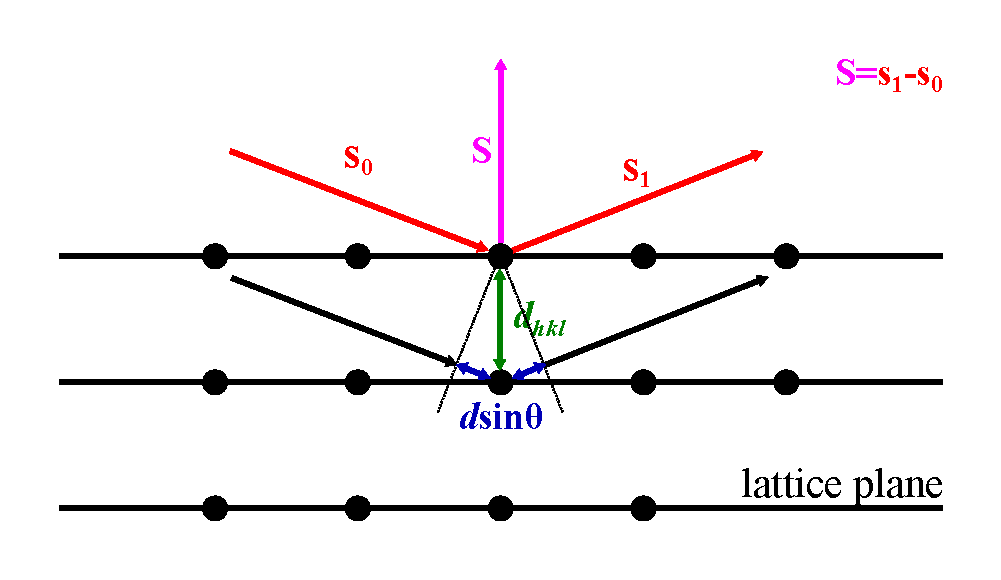
\includegraphics[width=0.7\textwidth]{introduction_bragg.pdf}
    \caption[Schematic of Bragg scattering]{Schematic of Bragg scattering.}
    \label{fig:introduction_bragg}
\end{figure}

It should be noted that \cref{eq:structure_factors} is a simplification of the problem at hand. In reality, instrument and experimental corrections need to be applied to the structure factor equation. A correction factor for each experiment-dependent parameter needs to be applied to the structure factor equation. However, in the scope of this work the details of such correction factors do not need to be discussed.

Since complex structure factors describe the molecular structure in the reciprocal space domain, the conversion to the real space domain in form of electron density is required. This can be conveniently done through the bijective Fourier transform, which allows the conversion of complex structure factors to electron density and vice versa without the loss of any information \cite{Rupp2010-nc}. Thus, electron density can be obtained from the complex structure factors using \cref{eq:electron_density}. The normalisation factor $1/V$ ($V$ represents the volume of the unit cell) provides the correct units for the electron density $\rho(x,y,z)$.

\begin{equation}
    \rho(x,y,z)=\frac{1}{V}\sum_{h=0}^{+\infty}\sum_{k=-\infty}^{+\infty}\sum_{l=-\infty}^{+\infty}\boldsymbol{F}(hkl)\cdot \exp\left(-2\pi\\i(hx+ky+lz)\right)
    \label{eq:electron_density}
\end{equation}
\equations{Mathematical expression of Electron Density}

\subsection{From crystal to structure}
In X-ray crystallographic experiments, X-ray radiation is measured using light detectors. However, the measurement taken is incomplete. Light detectors only capture the intensity of the scattered X-ray photons but crucially lose the phase information. The latter is essential for atomic reconstruction of the crystallised molecule, and thus needs to be obtained. In \gls{mx}, experimentalists have a number of alternative techniques to compensate for the lost phase information. 

Prior to the big advances in computing power and the successful elucidation of many protein structures, \gls{mx} crystallographers primarily recovered the lost phase information through Direct Methods or Experimental Phasing \cite{Rupp2010-nc}. Today, the most popular method to recovering the lost phase information is \gls{mr} \cite{Rossmann2001-yw,Rossmann1990-am}. In a \Gls{mr} search, a known structure (`search model') similar to the unknown is relocated in the unit cell until the solution with the best fit between calculated and observed diffraction data is obtained \cite{Rupp2010-nc}. A 6-dimensional search, i.e. a simultaneous rotation and translation search, is possible \cite{Kissinger1999-ho,Glykos2000-gc,Read2001-nu}, but is computationally very expensive and less suitable for challenging cases. In comparison, most modern crystallographic applications opt for two distinct sub-searches, the rotation search to orient the search model within the unit cell followed by the translation search to locate it \cite{Rupp2010-nc}. The benefits over a combined search include search-specific target functions that enable increased sensitivity and additional terms to compensate for imperfect data. 

The most successful \gls{mr} algorithms perform the rotation and translation searches using Patterson methods or Maximum Likelihood functions. Patterson methods --- originally developed by \textcite{Rossmann1962-ou} --- rely on the use of a map of vectors between the scattering atoms, which can be determined for the calculated and observed structure factor amplitudes. Patterson vectors can be subclassed as intra- and inter-molecular vectors. A distinct separation of the observed vectors is impossible. However, inter-molecular vectors appear further away from the central peak of the self-vector (vector from atom to itself) in the Patterson map \cite{Rupp2010-nc}. The calculated Patterson vectors for the search model allow for a clearer distinction between the intra- and inter-molecular vectors. If the search model is placed in a large unit cell, then inter-molecular vectors must scale with the unit cell dimension \cite{Rupp2010-nc}. Ultimately, using the intra-molecular Patterson vectors, the search model can be oriented against the experimentally determined Patterson vectors. In a similar manner, the inter-molecular vectors can be used to identify the correct translation of the search model. Patterson methods are very sensitive to small orientation errors of the search model \cite{Rupp2010-nc}. Thus, orientations with the highest vector peak overlaps are trialed in the subsequent translation search. Given that Patterson methods operate by Patterson vector comparisons in rotation and translation searches, these methods do not require search-model-derived phases.

In comparison to the Patterson methods, Maximum Likelihood methods do not rely on inter-atomic vectors in Patterson maps. Instead, Maximum Likelihood methods make use of Bayes' theorem \cite{Bayes1763-ox} to compare calculated structure factors and observed structure factor amplitudes directly \cite{Read2001-nu}. Bayes' theorem in crystallographic Maximum Likelihood methods is applied to compute the likelihood that an experimental value is observed given the current search model. The maximal likelihood indicates the optimal orientation and translation of the search model given the observed experimental data. Since the search model likelihood term is the product of many individual probabilities, which are difficult to represent computationally due to floating point representations, the log of the likelihood is commonly used \cite{Rupp2010-nc}. The major advantage of Maximum Likelihood methods over Patterson methods centres on the more realistic target functions, which consider errors and incompleteness of the search model, apply bulk solvent correction and conduct multi-model searches \cite{Read2001-nu}. The latter is of particular relevance since the Maximum Likelihood rotation function can thus consider already placed search models in a fixed position whilst trialling additional ones \cite{Storoni2004-ed}, which proves to be a major advantage over Patterson methods.  Furthermore, likelihood target functions can consider the structural variance of multiple superposed models in an ensemble search model, which is used to weight structure factors at the various positions to improve the overall likelihood term \cite{Read2001-nu}. 

The initial electron density map --- regardless of its determination by \gls{mr} or Experimental Phasing --- is almost always inaccurate. In \gls{mr}, inaccuracies arise from experimental errors, model incompleteness, low signal-to-noise or model bias. Thus, approaches for improving the phases used to calculated the initial electron density map have been developed and are routinely applied in \gls{mx}. Density modification describes a set of methods that improve the obtained electron density typically by applying statistical corrections to electron density distributions. These corrections are based on prior knowledge or assumptions of the physical properties of macromolecular structures \cite{Rupp2010-nc}. This process can transform initially poor or uninterpretable electron density maps to high quality ones. Three predominant density modification approaches exist: solvent flattening, histogram matching and the ``sphere-of-influence'' method. Solvent flattening is an approach was first proposed by \textcite{Wang1985-zu}. In solvent flattening, the disorder in the solvent region in a protein crystal is exploited, which differs in electron density from macromolecule-containing regions. If solvent electron density is set to a constant, then it is essentially flattened which will result in improved structure factors with improved phases and thus improved electron density. Histogram matching \cite{Lunin1988-lx} exploits the defined characteristics of an electron density distribution determined from sets of proteins at the same resolution, irrespective of individual structural details. The electron density distribution for noisy maps are Gaussian-shaped. In contrast, the electron density distribution of a feature-defined map is positively skewed. Thus, attempting to improve the Gaussian-shaped electron density distribution to better match the positively skewed shape results in overall improvements to the electron density. The ``sphere-of-influence'' method was introduced by \textcite{Sheldrick2002-tx} and classifies solvent and protein electron density by observing its variance across the shell surface of a 2.42\AA\ sphere (dominant 1-3 atom distance in macromolecular structures). If the sphere is positioned in the disordered solvent region typically found in inter-molecular channels, the density variance will be low. Thus, this approach allows to smoothen solvent-containing regions of the electron density \cite{Sheldrick2002-tx}. Independent of the density modification strategy applied, it is important to understand that improvements to the electron density map anywhere lead to improvements everywhere by transferral of information from one part of the map to another \cite{Terwilliger2000-sz}.

A second approach to improving the initial electron density is termed Refinement. Iteratively, the placed search model is optimised to better explain the experimentally observed data. This optimisation problem is typically broken down into three main steps: the definition of the model parameters, the scoring function and the optimisation method. The model parameters describe the crystal and its content and can be subdivided into atomic and non-atomic model parameters \cite{Afonine2012-bg}. These parameters combined are used to score the current model. The scoring function relates the experimental data to the model parameters. The scoring function contains two primary terms, the refinement data target and an \textit{a priori} knowledge term. The former defines a target function that assesses the similarity between calculated and experimental structure factors. The target function is commonly a Maximum Likelihood-based function that considers missing or incomplete data \cite{Murshudov2011-ww,Afonine2012-bg}. The \textit{a priori} knowledge term in the scoring function defines the properties of a good model by including stereochemical property terms. Lastly, optimisation methods provide tools to vary the model parameters to better fit the experimental data. Different optimisation techniques can be used depending on the severity of model parameter alteration, which generally depend on the entrapment of states in local energy minima. Model parameterisation and its scoring against the predefined scoring function combined with model optimisation form a refinement macrocycle, which is iteratively used to optimise a model's fit to the experimental data. This ultimately improves both the electron density map interpretability and model quality. \gls{mx} refinement can be performed in structure-factor-based reciprocal space and electron-density-based real space \cite{Afonine2012-bg}. A combination allows global and local refinement strategies and enables grid-like searches to optimise the model parameters until convergence.

Once initial phase information is improved through refinement and/or density modification, attempts can be made to build atomic model coordinates into the electron density map. This process is typically coupled with refinement or density modification to iteratively improve the quality of the partially built model and the electron density map \cite{Rupp2010-nc}. A small number of distinct algorithms are currently used to automatically build atomic coordinates into electron density: main-chain autotracing \cite{Sheldrick2010-cx}, fitting pseudo-atoms into electron density \cite{Lamzin2001-cn}, or fitting reference coordinates with similar electron density maps \cite{Terwilliger2004-ig,Cowtan2006-xv}. In essence, all algorithms attempt to maximise the number of correctly identified and placed atomic coordinates into available electron density. Whilst autotracing solely builds main-chain polypeptides, the other two approaches rely on sequence information to also build side-chains. Independent of the complexity of the model building task, the higher the resolution and the more complete the initial starting model, the less ambiguous and challenging this task becomes \cite{Rupp2010-nc}. 

\subsection{Unconventional Molecular Replacement}
The process of macromolecular structure determination via conventional \gls{mr} has been outlined previously. Search models are typically derived from structural homologs identified by sequence identity to the crystallised target \cite{Rupp2010-nc}. However, homologous structures are not always available or impossible to identify by current approaches. Experimental phasing approaches to circumvent the absence of \gls{mr} templates can be expensive, unsuccessful and very challenging for certain protein targets, and thus remain infeasible to pursue at times. Under such circumstances, alternative approaches are required, which are referred to as ``unconventional'' \gls{mr} approaches from here onwards. The unconventional \gls{mr} approach most relevant to the work presented in this thesis utilises the 3-dimensional structure prediction of a protein target starting from its sequence \cite{Qian2007-vo,Rigden2008-vo,Das2009-uz}. Although two distinct methods exist to predict the protein structure of a target sequence, homology modelling and \textit{ab initio} structure prediction, only the latter is relevant to this work since the former relies on homologous structures.
 
\section{\textit{Ab initio} protein structure prediction} \label{sec:introduction_structure_prediction}
The folding of protein structures is commonly described by the folding funnel hypothesis \cite{Leopold1992-yf}. It assumes that the native state of a protein fold corresponds to its global minimum free-energy state along its energy surface (\cref{fig:introduction_foldingfunnel}) \cite{Anfinsen1973-in}. \textit{In silico} protein folding experiments attempt to find this lowest free-energy state of the protein fold. However, to unambiguously identify this state sampling of all polypeptide chain conformations is necessary. In theory, sampling of all conformations for a 100-residue protein takes in the order of approximately $10^{52}$ years ($10^7$ configurations with $10^{-11}$ seconds per configuration), yet \textit{in vivo} an equivalent polypeptide chain folds in milliseconds to seconds \cite{Levinthal1969-bn,Karplus2011-jh}. This paradox --- termed the Levinthal paradox \cite{Levinthal1969-bn} --- created the basis for the folding funnel hypothesis.  

\begin{figure}[H]
    \centering
    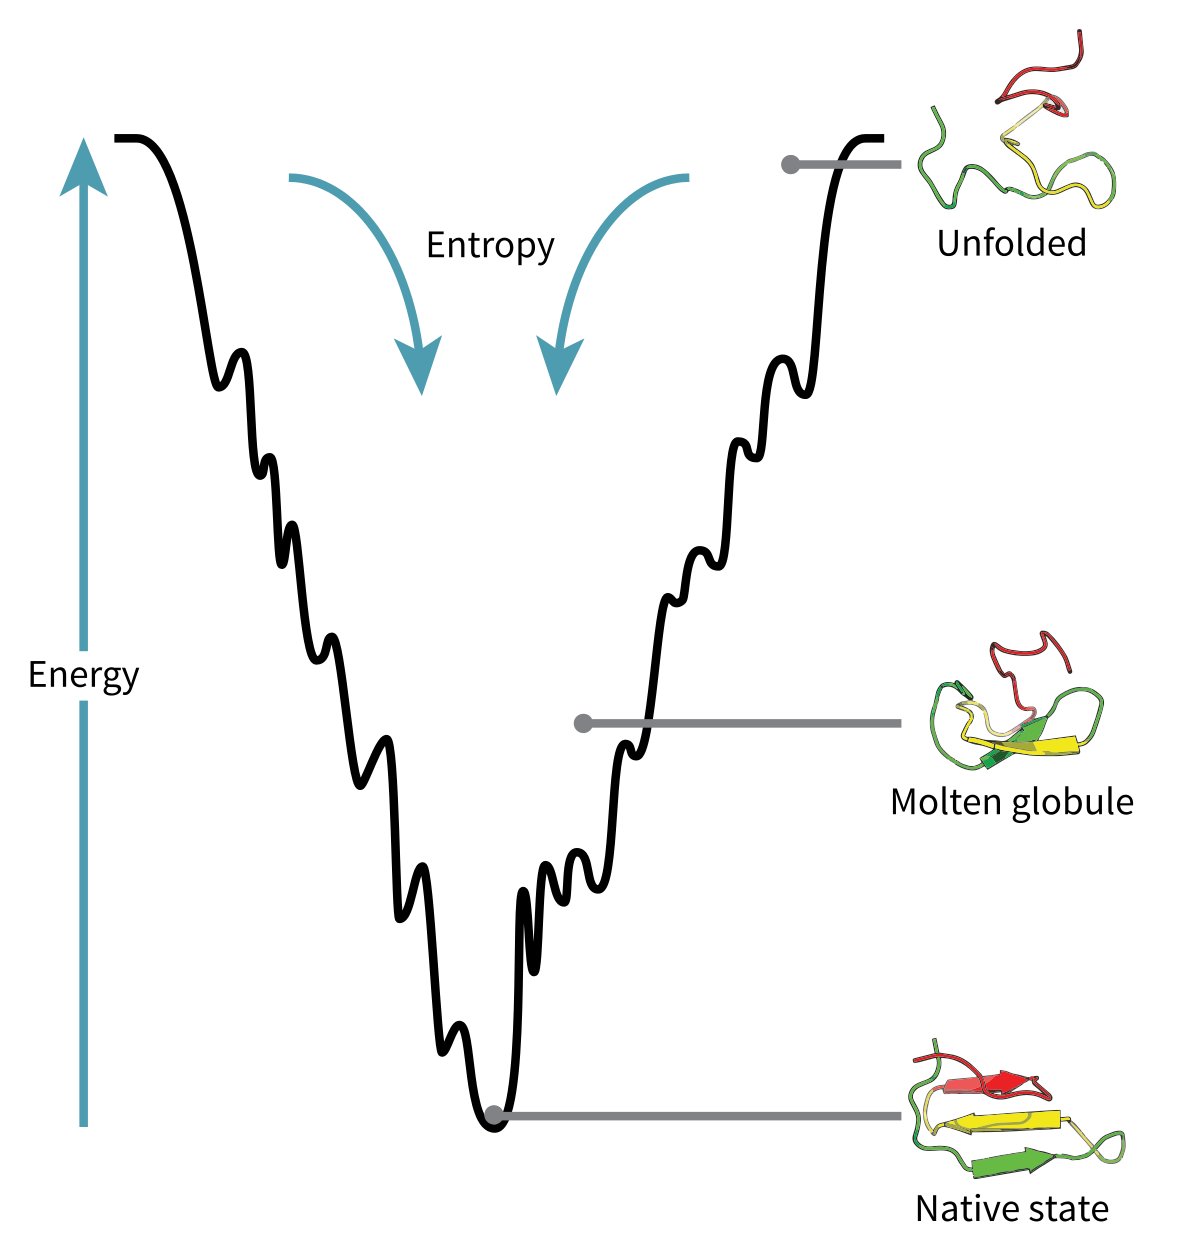
\includegraphics[width=0.5\textwidth]{introduction_foldingfunnel.png}
    \caption[Schematic of the folding funnel hypothesis]{Schematic of the folding funnel hypothesis \cite{Leopold1992-yf}. Diagram produced by \textcite{Wikipedia-FoldingFunnel} contributors.}
    \label{fig:introduction_foldingfunnel}
\end{figure}

In \textit{ab initio} protein structure prediction, the tertiary structure of a protein is predicted using its primary structure alone. This problem is in its nature identical to finding the lowest free-energy state along a protein's energy landscape. However, in an attempt to avoid the Levinthal paradox, different knowledge- and physics-based energy functions coupled with a variety of conformational search sampling algorithms are employed \cite{Lee2017-oc}. 

Physics-based energy functions use physiochemical force fields typically coupled with Molecular Dynamics simulations to sample the folding trajectory of a protein sequence (true physics-based approaches are computationally intractable because quantum mechanics models would need to be used). Force fields describe parameter sets used to calculate energy potentials for a system of atoms in a simulation run, and include potentials, such as van der Waals and electrostatic interactions \cite{Lee2017-oc}. In the context of \textit{ab initio} protein structure prediction, pure physics-based approaches are often less favourable, because the computational complexity to find the lowest free-energy state of a large protein structure remains intractable without the use of supercomputers.

Knowledge-based energy functions rely on empirical energy terms derived from statistics and regularities of experimentally determined structures \cite{Lee2017-oc}. These energy terms can be subdivided into two types, the generic or sequence-independent terms and amino-acid or sequence-dependent terms \cite{Skolnick2006-uv}. The former include terms to describe the backbone hydrogen-bonds and local backbone stiffness of a polypeptide chain. The sequence-dependent terms include terms such as pairwise residue contact potential, distance-dependent atomic contact potential, and secondary structure propensities. However, predicting local or global tertiary structure of a protein sequence using empirical energy terms alone is very difficult. Subtle differences in the local and global environment of a primary structure alongside the subtle differences in initial folds leading to common secondary structure features are very difficult to reproduce in a modelling scenario. Thus, knowledge-based energy functions are often coupled with the assembly of fragments extracted from other protein structures to predict the unknown tertiary structure of the target sequence \cite{Lee2017-oc}. 

The most successful \textit{ab initio} structure prediction protocols use knowledge-based and physics-based energy functions combined with fragment-assembly-based conformational searches to find the lowest free-energy state \cite{Rohl2004-dj,Xu2012-jf,Blaszczyk2013-nx,Kosciolek2014-bt,De_Oliveira2017-sg}. Structural fragments of varying lengths (typically 3-20 residues) are extracted from existing protein structures \cite{Abbass2015-qk,Shen2013-wh,Li2008-xu,Kalev2011-sz,Bhattacharya2016-ix,Wang2017-ka,De_Oliveira2015-kb,Gront2011-sv}. These fragments are used in a Monte Carlo simulation to search the conformational space of the polypeptide chain for low free-energy states \cite{Metropolis1949-kp}. The insertion of overlapping fragments results in the replacement of torsion angles either at random positions or sequentially from predefined starting position (such as N- or C-termini). Each move is scored against the Metropolis criterion \cite{Metropolis1949-kp} consisting of knowledge-based and physics-based terms. The Metropolis criterion is typically defined to accept fragment insertions that lower the free-energy term of a decoy, whilst sometimes accepting insertions that increase the free-energy term to escape local energy minima. If the insertion of a fragment passed the Metropolis criterion, the related torsion angles are accepted and integrated in the polypeptide chain for the next fragment-insertion iteration. This process is repeated until convergence of the decoy, i.e. no lower free-energy state can be found. In all routines, these steps are independently repeated thousands of times to create a pool of decoys. 

In order to identify the correct fold amongst the thousands of generated decoys, clustering approaches are often used in combination with \textit{ab initio} protein structure prediction protocols. \textcite{Shortle1998-fq} identified that the most-similar decoy to the native structure is most often the centroid (decoy with most neighbours in the cluster) of the largest cluster. Further studies showed that the selection of those centroid decoys helps to identify the most native-like folds amongst the many thousands generated \cite{Zhang2004-uz,Bradley2005-lw,Oldziej2005-qp}. Some protocols use clustering as an intermediate or final step to identify decoys for which it will perform more computationally demanding all-atom refinement \cite{Bradley2005-lw} or other decoy hybridisation techniques \cite{Zhang2004-uc,Xu2012-jf,Yang2015-oc} to further approach the native-like fold \cite{Kryshtafovych2016-aq}.

Despite active research in \textit{ab initio} protein structure prediction over decades, all approaches struggle with accurate predictions for larger protein domains (chain lengths $>150$ residues) \cite{Bradley2005-lw,Tai2014-rz,He2013-gm,Kinch2011-py}. The major challenge arises from the sampling of the conformational space since incorrect local changes influence the global structure. Furthermore, \textbeta-sheets are inherently difficult to predict given that \textbeta-strands in fragment-based approaches are inserted one at a time yet rely on the hydrogen-bond network typically found in \textbeta-sheets to reduce the overall energy of the decoy \cite{Rohl2004-dj}. To address this issue, \textcite{Lange2012-yh,Raman2010-xv,Gobl2014-gc} started to use \gls{noe} data as residue-residue distance restraints to reduce the sampling space of conformations, which enabled high-resolution predictions of tertiary structure for longer proteins. Although successfully applied in the aforementioned examples, experiments to collect \gls{noe} data are costly, challenging and intractable for larger multi-domain targets. To avoid this problem yet obtain similarly useful information on spatial proximity of amino acids in a protein fold, researchers started to exploit residue-residue contact information, which enables accurate \textit{ab initio} structure prediction for longer polypeptide chains \cite[e.g.,][]{Marks2011-os,Michel2014-eg,Kosciolek2014-bt,Ovchinnikov2015-tn,Ovchinnikov2016-jj,Michel2017-xh,De_Oliveira2017-sg,Ovchinnikov2017-nd,Wang2017-rx}.

\section{Residue-residue contact prediction} \label{sec:introduction_contact_prediction}
The use of predicted residue-residue contact information to reduce the conformational search space in \textit{ab initio} protein structure prediction relies on accurate identification of amino acids in close spatial proximity. Today, such identification can be detected from sequence information alone by either \gls{dca} or \gls{sml} algorithms.

\subsection{Direct Coupling Analysis}
\Acrlong{dca} uses protein sequence information to identify coordinated changes of amino acids in sequences of a protein family (\cref{fig:introduction_covariance}). These coordinated changes are caused by evolutionary pressure to maintain residue interactions important for protein structure and function. However, original attempts to detect covariation signal from sequences in a protein family were unsuccessful for many years \cite{Taylor1994-es,Gobel1994-rp,Neher1994-qn,Shindyalov1994-yp}. The applied local statistical model suffered from numerous drawbacks, including the loss of covariation signal due to phylogenetic dependencies, limited availability of sequence data, and the potentially false assumption that truly coevolved residues are in close proximity in sequence space \cite{Pollock1997-os,Lapedes1999-cg,Lapedes2012-tu}. Implementations of the local statistical model used raw covariation frequencies between pairs of positions in the sequence alignment. This further poses issues since successful distinction between ``direct'' casual (A-B and B-C) and ``indirect'' transitive (A-C) correlations is essential for successful protein structure prediction yet cannot be separated by frequency comparisons. 

\begin{figure}[H]
    \centering
    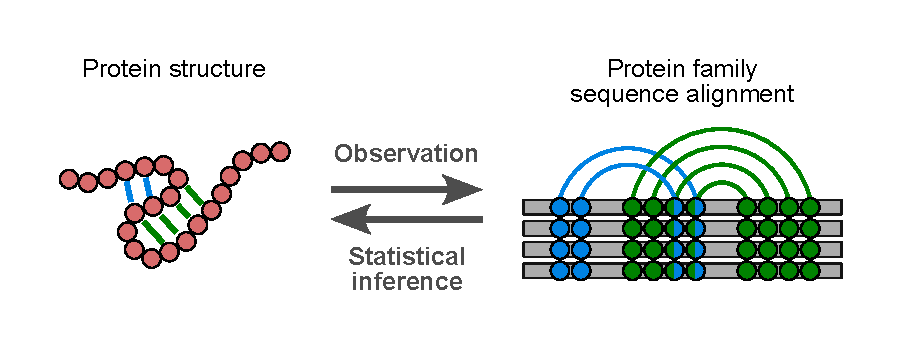
\includegraphics[width=1.0\textwidth]{introduction_covariance.pdf}
    \caption[Schematic of inference of covariance signal]{Schematic of inference of covariance signal originating from evolutionary pressure in protein tertiary structures and encoded in its family's sequence alignment (adapted from \cite{Simkovic2017-xs}).}
    \label{fig:introduction_covariance}
\end{figure}

\textcite{Lapedes1999-cg} proposed the use of a global statistical model to infer correlations of residue pairs to circumvent the main problem of decoupling causal and transitive correlations. However, it was not until a decade later before first implementations of the global statistical model surfaced to successfully disentangle these types of correlations \cite{Weigt2009-sx,Burger2010-ee,Balakrishnan2011-wh,Marks2011-os,Morcos2011-lk,Jones2012-ks,Ekeberg2013-ay,Kamisetty2013-le,Seemayer2014-zp}. The use of a global statistical model achieves successful disentanglement by inferring a probabilistic description of the sequence alignment that best explains observed correlations using underlying causal couplings between positions \cite{Hopf2017-pp}. Such couplings can be inferred by maximising the likelihood of observing the sequences in the alignment under the maximum entropy probability model. In other words, by considering all amino acid pair positions simultaneously, causal and transitive couplings can be successfully disentangled \cite{Ekeberg2013-ay}.

The pairwise probabilistic model $P(\boldsymbol{\sigma})$ of the amino acid sequence $\boldsymbol{\sigma}=\left(\sigma_1,\sigma_2,\dots,\sigma_N\right)$ of length $N$ is defined in \cref{eq:potts_model}, which contains the amino acid configuration constraints $\sigma_i$ and $\sigma_j$ at positions $i$ and $j$, the single-site conservation bias term $h_i$, and co-conservation term $J_{ij}$ between position pairs $i,j$. 

\begin{equation}
    P(\boldsymbol{\sigma})=\frac{1}{Z}\exp\left(\sum_{i=1}^{N}h_i\left(\sigma_i\right)+\sum_{1 \leqslant i < j \leqslant N}J_{ij}\left(\sigma_i, \sigma_j\right)\right)
    \label{eq:potts_model}
\end{equation}
\equations{Potts model}

\begin{equation}
    Z=\sum_{\boldsymbol{\sigma}}^{ }\exp\left(\sum_{i=1}^{N}h_i\left(\sigma_i\right)+\sum_{1 \leqslant i < j \leqslant N}J_{ij}\left(\sigma_i, \sigma_j\right)\right)
    \label{eq:potts_model_partition_function}
\end{equation}
\equations{Partition function of Potts model}

The partition function $Z$ (\cref{eq:potts_model_partition_function}) acts as normalising constant, and additionally has the property to maximise the entropy in the probabilistic model. However, the computation of $Z$ is intractable for the feature space found in \gls{dca} since the number of summations in $Z$ exponentially increases with $N$ for all 20 amino acid configurations. Thus, approximations of $Z$ are typically used, which were shown to lead to precise covariance predictions \cite{Ekeberg2013-ay}.

Over the last decade, numerous approximations for the parameter inference of $P(\boldsymbol{\sigma})$ have been implemented, which include gradient ascent with Monte Carlo sampling \cite{Lapedes2012-tu}, message passing \cite{Weigt2009-sx}, mean-field \cite{Marks2011-os,Morcos2011-lk,Jones2012-ks,Stein2015-cw}, and pseudolikelihood maximisation \cite{Balakrishnan2011-wh,Ekeberg2013-ay,Kamisetty2013-le,Seemayer2014-zp,Hopf2015-vf}. However, it is the latter that has proven to be most successful, and is thus at the core of most widely-used applications. In pseudolikelihood maximisation \gls{dca} approaches, the full likelihood for each sequence position $i$ in $\boldsymbol{\sigma}$ across all sequences in the alignment is approximated by a product of conditional likelihoods (\cref{eq:covariance_pseudolikelihood_approximation}) \cite{Hopf2017-pp}.

\begin{equation}
    \mathcal{L}\left(\mathbf{h},\mathbf{J}\right)=\prod_{\sigma\in\Sigma}P\left(\sigma\rvert\mathbf{h},\mathbf{J}\right)\approx\prod_{i=1}^{N}P\left(\sigma_i\rvert\sigma\backslash\sigma_i,\mathbf{h},\mathbf{J}\right)
    \label{eq:covariance_pseudolikelihood_approximation}
\end{equation}
\equations{Covariance pseudo-likelihood approximation}

\Cref{eq:covariance_pseudolikelihood_approximation} describes the conditional probability of observing amino acid ($\sigma_i$) in position $i$ given all other amino acids ($\sigma\backslash\sigma_i$) in $\boldsymbol{\sigma}$. This leads to the cancellation of the partition function $Z$, and instead normalises locally over all possible 20 amino acid configurations at each site $i$. The parameters $\mathbf{h}$ and $\mathbf{J}$, which minimise \cref{eq:covariance_pseudolikelihood_approximation}, are identified using iterative optimisation algorithms \cite{Hopf2017-pp}. Typically, regularisation terms are also added to \cref{eq:covariance_pseudolikelihood_approximation} to avoid overfitting of the input data \cite{Hopf2017-pp}.

The positional constraint matrices $J_{ij}$ for all amino acid ($k$) pairs across all combinations of $\sigma_i$ and $\sigma_j$ in $\boldsymbol{\sigma}$ need be summarised to a coupling score between $\sigma_i$ and $\sigma_j$. The Frobenius norm is the preferred summary statistic (\cref{eq:frobenius_norm}), and applied to a row- and column-means-centered coupling matrix $J'_{ij}$ (\cref{eq:row_column_cent_mat}). Furthermore, \gls{apc} is applied to remove background couplings that arise due to noise from phylogenetic relationships between sequences to provide the final \gls{ec} score (\cref{eq:evolutionary_coupling_score}) \cite{Dunn2008-ao,Jones2012-ks,Ekeberg2013-ay,Kamisetty2013-le,Seemayer2014-zp}.

\begin{equation}
    J'_{ij}=J_{ij}(k,l)-J_{ij}(\cdot,l)-J_{ij}(k,\cdot)+J_{ij}(\cdot,\cdot)
    \label{eq:row_column_cent_mat}
\end{equation}
\equations{Matrix centering}

\begin{equation}
    FN(i,j)=\sqrt{\sum_{k}\sum_{l}J'_{ij}(k,l)^2}
    \label{eq:frobenius_norm}
\end{equation}
\equations{Frobenius norm}

\begin{equation}
    EC(i,j)=FN(i,j)-\frac{FN(i,\cdot)FN(\cdot,j)}{FN(\cdot,\cdot)}
    \label{eq:evolutionary_coupling_score}
\end{equation}
\equations{Evolutionary coupling score}

Despite the great precision achievable by \gls{dca} algorithms, such algorithms suffer from one major drawback. All covariance-based algorithms rely on the availability of a sufficiently large and diverse \gls{msa} for the protein family of interest. Although the minimum number of sequences required per \gls{msa} might be target- and algorithm-dependent, early works suggested a minimum requirement of $>1000$ sequence homologs \cite{Jones2012-ks,Marks2012-ko,Andreani2015-qn}. Simultaneously, \textcite{Marks2011-os} and \textcite{Kamisetty2013-le} recommended a more sequence-specific length-dependent factor, whereby the sequence count in the alignment should exceed at least five times the protein length for precise predictions. Whilst those earlier suggestions permit crude estimations of the likelihood of obtaining precise contact predictions, researchers realised that highly redundant \gls{msa}s could surpass such a threshold yet not provide enough diversity typically required for covariance-signal detection. Thus, the measure of alignment depth (also termed \gls{meff}) was introduced to capture both the sequence count and diversity in a given alignment \cite{Morcos2011-lk,Hopf2012-zl,Skwark2014-qp,Jones2015-vq}. Although target- and algorithm-dependent thresholds persist, a minimum of 100-200 effective sequences are typically required \cite{Skwark2014-qp,Jones2015-vq}. Furthermore, individual weights used to calculate the alignment depth are widely used in covariance-based algorithms to reweight individual sequences \cite{Ekeberg2013-ay}. The benefit is twofold: an important assumption of \cref{eq:potts_model} that all samples are independent is satisfied and the phylogenetic effect of non-independently evolved sequences is simultaneously reduced \cite{Ekeberg2013-ay}. Similar results may be achieved by removing redundant sequences prior to \gls{dca}. However, this may result in the loss of information by the requirement of selectively choosing a single representative sequence.

\subsection{Supervised Machine Learning}
Unlike \gls{dca} approaches, \gls{sml} algorithms do not rely on the availability of homologous sequences to predict residue-residue contacts. Instead, \gls{sml} models are trained on a variety of sequence-dependent and sequence-independent features to infer contacting residue pairs \cite{Du2016-hl,Gonzalez2013-wg,Shackelford2007-iz,Cheng2005-da,Zhang2016-px,Wang2013-wi}. Broadly speaking, such \gls{sml} algorithms rely on the analysis of sequence-based features, such as secondary structure, and sequence profiles. \Gls{sml} algorithms suffer from an inability to distinguish between residue pairs that form direct and indirect contact pairs, similar to earlier implementations of covariance-based methods. However, pure \gls{sml}-based algorithms are not relevant to the work described in this thesis, and thus not further discussed. It is worth noting though that covariance-based algorithms outperform pure \gls{sml} algorithms for protein families with many homologous sequences, whilst \gls{sml} algorithms outperform \gls{dca} algorithms for families with fewer homologous sequences \cite{Skwark2014-qp,Wang2013-wi,Ma2015-vo}. 

\subsection{Contact metapredictors}
The most recent approaches in residue-residue contact prediction use combinatorial approaches to exploit information from \gls{dca} and \gls{sml} approaches. Metapredictors commonly use \gls{sml} approaches as priors \cite{Ovchinnikov2015-tn} or posteriors \cite{Skwark2014-qp,Jones2015-vq,Adhikari2017-kt,He2017-fn,Michel2017-pm,Wang2017-rx} in addition to \gls{dca} algorithms. Furthermore, metapredictors use multiple input \gls{msa}s and/or \gls{dca} algorithms to further enhance the prediction precision. In most cases, metapredictors outperform their individual approaches and improvements are most noticeable for targets with lower alignment depths \cite{De_Oliveira2017-gj,Wuyun2016-hh,Wang2017-rx}.

\section{AMPLE}
The major challenge in unconventional \gls{mr} is to address cases where a search model cannot easily be derived from the \gls{pdb}, because structures homologous to the target have not been determined or cannot be identified. The ensemble search model preparation pipeline AMPLE (\textbf{A}b initio \textbf{M}odelling of \textbf{P}roteins for mo\textbf{LE}cular replacement) --- based on the work of \textcite{Rigden2008-vo} --- attempts to tackle this challenge by utilising structural information from a variety of sources, such as \textit{ab initio} structure predictions \cite{Bibby2012-lm,Keegan2015-zb,Simkovic2016-wk,Thomas2015-wu,Thomas2017-sh}, \gls{nmr} ensembles \cite{Bibby2013-cp}, and single \cite{Rigden2018-zt} or multiple distant homologs \cite{Bruhn2014-aa,Hotta2014-me}. 

AMPLE's algorithm attempts to identify a structurally shared core amongst the initial starting structures. The idea is simple, if a shared core is present amongst a set of many structures, the likelihood of its presence in the unknown target is high. However, the rationale for identifying the shared core changes given the origin of the starting structures. In the case of clustered \textit{ab initio} decoys, local regions inaccurately predicted can be determined by the structural divergence within each cluster. The removal of these regions reduces the error in the set of structure predictions, and if the prediction was accurate it should elucidate a conserved structural core \cite{Bibby2012-lm}. Similarly, in \gls{nmr} ensembles locally divergent regions are the result of greater flexibility in solution, and often these regions differ most from the corresponding crystal structure. Thus, removal of such flexible regions increases the likelihood of determining a structurally similar, conserved subfold suitable as \gls{mr} search model \cite{Bibby2013-cp}. If only a single distant homolog is available, a structural ensemble can be generated reflecting the innate flexibility of the starting structure. Since rigidity and evolutionary conservation are correlated \cite{Yeh2014-vl, Shih2012-gh}, this flexibility can be used as a proxy similar to \gls{nmr} ensembles to drive trimming for identification of a more rigid, shared core \cite{Rigden2018-zt}. Multiple distant homologs differ to the previous three examples because the shared core is most likely a small subfold present in all homologous structures. Successful identification of this subfold or super-secondary-structure motif, which often contains the functional unit of the protein family and is also likely to be present in the target, could be sufficient for structure determination \cite{Bruhn2014-aa,Hotta2014-me}. 

\begin{figure}[H]
    \centering
    \includegraphics[width=1.0\textwidth]{introduction_ample.pdf}
    \caption[Cluster-and-truncate approach employed by AMPLE]{Schematic representation of the cluster-and-truncate approach employed by AMPLE.}
    \label{fig:introduction_ample}
\end{figure}

In each case, AMPLE attempts to identify such a shared core by employing a cluster-and-truncate approach (\cref{fig:introduction_ample}) \cite{Bibby2012-lm}. The latter can be separated into three main parts: (i) clustering of starting models to identify subsets of similar folds (only applicable for \textit{ab initio} structure predictions), (ii) incremental truncation of each cluster or collection of structures by its structural variance or other per-residue metric, and (iii) subclustering of each truncated set of starting structures to create subgroups with varying levels of structural diversity. The incremental truncation of each cluster is typically done at 20 different levels (i.e. 5\% intervals) based on the inter-residue variance score \cite{Theobald2006-qj}. Sub-clustering is performed under three different \gls{rmsd} thresholds (1, 2 and 3\AA). AMPLE requires each ensemble search model to contain at least two starting structures, and if this requirement is satisfied each ensemble search model is stripped to poly-alanine side-chains (all-atom and reliably-modelled side-chain \cite{Krivov2009-ex} treatments are also available and were used by default in previous versions). This leads to the unbiased generation of a large number of ensemble search models, which cover a great diversity of its original structural information, and hopefully capture in one or more of those generated search models the shared core necessary for successful structure solution. Furthermore, AMPLE's unbiased ensemble search model generation protocol often identifies local features amongst sets of less accurate \textit{ab initio} protein structure predictions, which are sufficient for structure determination. 

Beyond the generation of ensemble search models, AMPLE also integrates the automated \gls{mr} pipeline MRBUMP \cite{Keegan2018-kn}. In AMPLE, MRBUMP's structure determination features are of particular interest. It employs PHASER \cite{McCoy2007-mp} and MOLREP \cite{Vagin2010-ux} for \gls{mr}, refines the \gls{mr} solutions with REFMAC5 \cite{Murshudov2011-ww}, uses SHELXE for density modification and main-chain tracing \cite{Thorn2013-le}, and attempts automated model building with ARP/wARP \cite{Cohen2007-wg} and BUCCANEER \cite{Cowtan2006-xv}. These features enable the sampling of each AMPLE-generated ensemble for its suitability as \gls{mr} search model.

\section{Aims}
In \cref{sec:introduction_mx,sec:introduction_structure_prediction,sec:introduction_contact_prediction}, the fundamental theories behind three major areas of research were outlined: \acrlong{mr} and the need for unconventional approaches, \textit{ab initio} protein structure prediction, and residue-residue contact prediction. AMPLE, a well-established pipeline in \gls{mx}, combines the former two to simplify structure solution of challenging or novel protein folds. However, the success of AMPLE's main idea, which generates ensemble search models from \textit{ab initio} structure predictions and is the focus of the work presented in this thesis, is heavily dependent on the quality of the initial \textit{ab initio} decoys, which are limited inherently by the computational complexity of finding the lowest free-energy state during sampling. Predicted residue-residue contact information, as described in \cref{sec:introduction_contact_prediction}, reduces the conformational search space in \textit{ab initio} structure prediction.

Therefore, the primary aim of the work presented in this thesis focused on exploring benefits and applications of residue-residue contact prediction to improving the approach AMPLE takes in unconventional \gls{mr}. Furthermore, work centred on the identification of other areas of application of residue-residue contact prediction to aid the structure solution process in unconventional \gls{mr}. To address these aims, the following steps were taken:

\begin{enumerate}
    \item In \cref{chap:proof_of_principle}, an initial proof-of-principle study was conducted to highlight the benefits of residue-residue contact prediction to AMPLE's \textit{ab initio} structure determination routine.
    \item In \cref{chap:rosetta_energy_functions}, the proof-of-principle study was expanded to explore the newly defined boundaries of AMPLE by exploring a diversity of metapredictors and ROSETTA energy protocols for introducing distance restraints into the \textit{ab initio} folding protocol.
    \item In \cref{chap:alternate_abinitio_protocols}, work was carried out to identify potential alternatives to AMPLE's recommended structure prediction protocol ROSETTA. Three alternative protocols --- SAINT2 \cite{De_Oliveira2017-sg}, FRAGFOLD \cite{Kosciolek2014-bt} and CONFOLD2 \cite{Adhikari2018-lj} --- were explored for potential benefits over ROSETTA.
    \item In \cref{chap:ample_decoys}, a study was carried out to explore the estimation of decoy quality by its satisfaction of predicted long-range contacts. Subsequent exclusion of the least accurate decoys was trialled as novel processing prior in AMPLE's cluster-and-truncate approach.
    \item In \cref{chap:ample_flib}, a pilot study was carried out to explore the potential of residue-residue contact prediction in identifying structural fragments or subfolds, specifically with the intend to use these identified structures as search models in \gls{mr}. 
\end{enumerate}


\chapter{Materials \& Methods}
\clearpage
% \section{Selection of datasets}
\subsection{ORIGINAL dataset} \label{sec:methods_dataset_original}
A test set of 21 globular protein targets was manually selected to include a range of chain lengths, fold architectures, X-ray diffraction data resolutions and \gls{msa} depths for contact prediction  (\cref{table:appendix_dataset_original}). The targets were chosen to include the three main fold classes: all-\textalpha, all-\textbeta, and mixed \textalpha-\textbeta\ (\textalpha/\textbeta\ and \textalpha+\textbeta). The target chain lengths cover a range from 62 to 221 residues. Each crystal structure contains a single molecule per asymmetric unit and the resolution of the experimental data is in range of 1.0 to 2.3\AA.

\subsection{PREDICTORS dataset} \label{sec:methods_dataset_predictors}
An unbiased selection of 27 non-redundant protein targets was selected using the following protocol. For target-specific details, please refer to \cref{table:appendix_dataset_predictors}.

The PFAM v29.0 \cite{Finn2016-zo} database was filtered for all protein families with at least one representative structure in the RCSB \gls{pdb} \cite{Berman2000-ua} database. Each representative had to have monomeric protein stoichiometry and its fold classified in the SCOPe v2.05 database \cite{Chandonia2017-vf}. Targets with fold assignments other than "a" (all-\textalpha), "b" (all-\textbeta), "c" (mixed \textalpha+\textbeta) or "d" (mixed \textalpha/\textbeta) were excluded to focus on regular globular protein folds. Each resulting protein target was screened against the RESTful API of the RCSB \gls{pdb} (\url{www.rcsb.org}) web server to identify targets meeting the following criteria: experimental technique is X-ray crystallography; chain length is $\geq100$ residues and $\leq250$ residues; resolution is between 1.3 and 2.3\AA; structure factor amplitudes are deposited in the \gls{pdb} \cite{Berman2000-ua} database; and there is only a single molecule in the asymmetric unit. The resulting protein structures were cross-validated against the \gls{pdbtm} \cite{Tusnady2005-ns} to exclude any possible matches. Subsequently, one representative entry was randomly selected for each PFAM family.

All PFAM family representatives obtained in the previous step were grouped by domain fold, target chain length and PFAM alignment depth (see \cref{eq:methods_meff}). Each target was sorted in one of three fold bins depending on their SCOPe fold assignment: all-\textalpha, all-\textbeta, and mixed \textalpha-\textbeta\ (\textalpha+\textbeta\ and \textalpha/\textbeta). Each target was further binned by chain length (derived from the deposited sequence in the RCSB \gls{pdb}) into three different bins: $[100, 150)$, $[150, 200)$, and $[200, 250]$. Lastly, each fold bin was also subgrouped by alignment depth, which was calculated for each sequence alignment of each PFAM family. Three bins were established: $[0, 100)$, $[100, 200)$, and $[200, \infty]$. Thus, all targets were grouped by fold class and further subgrouped by chain length or alignment depth.

In the final step, random targets were selected from each bin to obtain nine targets per fold sampling a spectrum of target chain lengths and alignment depths. To ensure similar samples across the fold classes, random PFAM entries were continuously picked from the fold bins until the mean target chain length and alignment depth of nine representatives of each fold class were within $\pm15$ of each other. This resulted in 27 targets in the final set.

\subsection{TRANSMEMBRANE dataset} \label{sec:methods_dataset_transmembrane}
The selection of this dataset was done by \textcite{Thomas2017-sh}. In summary, 13 non-redundant transmembrane protein targets were selected from the \gls{pdbtm} \cite{Tusnady2005-ns}, with a chain length of $<250$ residues and resolution of $<2.5$\AA. The final selection is summarised in \cref{table:appendix_dataset_transmembrane}. The target with \gls{pdb} ID 3u2f was removed from the original dataset described by \textcite{Thomas2017-sh} due to a high similarity with \gls{pdb} ID 2wie.

\section{Enhancement of \textbeta-sheet restraints} \label{sec:methods_bbcontacts_addition}
Structure prediction of \textbeta-strand containing protein targets \textit{ab initio} is a notoriously challenging task. \textbeta-strands, potentially far in sequence space, form a \textbeta-sheet in 3-dimensions. Since fragment-assembly algorithms work on the basis of randomly inserting one fragment at the time, the probability of \textbeta-sheet formation is much lower compared to \textalpha-helices. 

Recent advances in \textit{ab initio} structure prediction have seen great improvements in structure prediction quality through the use of predicted residue-residue contacts as distance restraints (see \cref{sec:introduction_contact_prediction}). However, little research has specifically focused on improvements to the structure prediction of \textbeta-sheet formation \cite{Hayat2015-ut}. To enhance the probability of \textbeta-sheet formation in \textit{ab initio} structure prediction, part of this thesis focused on a more general model to enrich restraints between \textbeta-strands to attempt better super-secondary quality in the final decoys.

A more general approach, compared to \textcite{Hayat2015-ut}, which focused exclusively on \textbeta-barrel proteins, was developed combining a starting set of contact pairs with a specifically-prepared set obtained from BBCONTACTS \cite{Andreani2015-qn}. A HHBLITS \cite{Remmert2011-kt} \gls{msa} was constructed using two sequence-search iterations with an E-value cutoff of $10^{-3}$ against the \texttt{uniprot20} database \cite{The_UniProt_Consortium2017-pb}. Redundant sequences were removed from the \gls{msa} to 90\% sequence identity using HHFILTER \cite{Remmert2011-kt}. Subsequently, the \gls{msa} was subjected to CCMPRED \cite{Seemayer2014-zp} for coevolution based contact prediction, which was chosen to reproduce the approach published by \textcite{Andreani2015-qn}. Alternative starting predictions might be provided although such approach was not tested within the scope of this work. Additionally to the contact prediction, the BBCONTACTS algorithms requires a secondary-structure prediction, which can be obtained using the \texttt{addss.pl} script \cite{Remmert2011-kt} distributed with the HHSUITE \cite{Soding2005-hw}. BBCONTACTS also requires a descriptor for the diversity of the original \gls{msa} \cite{Andreani2015-qn}, which is calculated using \cref{eq:methods_alndiversity}. Ultimately, the BBCONTACTS algorithm yields \textbeta-strand-specific contact predictions identified from the starting set of contacts.

The BBCONTACTS contact pairs were added to a base set of contact pairs usually obtained from a separate (meta-)predictor. The first step included the filtering of the predicted BBCONTACTS contact list to exclude any one- or two-pair \textbeta-strand contacts, i.e. sequences of contacts with less than three consecutive contact pairs, because those typically show a high \gls{fp} rate (Jessica Andreani, personal communication). The subsequent combination of the two sets of contact pairs was done by simple union of the lists; however, if a contact pair was in the intersection, a contact-pair related weight was doubled to allow subsequent modifications of the energy term in distance restraint creation. Furthermore, additional contact pairs were inferred if not present in the base set of contact pairs. The inference worked on the basis that any neighbouring contacts (i.e. $i,j\pm1$; $i,j\pm2$; $i\pm  1,j$; $i\pm2,j$) to contact $i,j$ must be present, and thus any missing such contacts were automatically added to the final set of contact pairs. 

\section{Evaluation of data}
This section defines and describes data validation and verification procedures and equations used throughout one or more studies presented in this thesis. These definitions serve as a reference and define naming conventions where appropriate. All of the sequence- and contact-related analysis routines are implemented in CONKIT \cite{Simkovic2017-us}.

\subsection{Sequence alignment data}
\subsubsection{Sequence alignment diversity}
The sequence diversity in a \gls{msa} can be described by the number of sequences ($M$) it contains divided by the sequence length of the target ($L$). The diversity metric was used in BBCONTACTS as input parameter \cite{Andreani2015-qn}. The \gls{msa} diversity $\eta$ is defined in \cref{eq:methods_alndiversity}.

\begin{equation}
    \eta=\frac{M}{L}
    \label{eq:methods_alndiversity}
\end{equation}
\equations{Sequence Alignment diversity}

\subsubsection{Sequence alignment depth}
Co-evolution based residue-residue contact prediction is dependent on an input \gls{msa} ideally containing all homologous sequences found in the queried database. However, the \gls{msa} needs a certain level of sequence diversity amongst the homologs to accurately capture the coevolution signal. The alignment depth --- often also referred to as \gls{meff} --- captures this diversity by computing the number of non-redundant sequences in the \gls{msa}.

\begin{equation}
    M_{eff}=\sum_{i}\frac{1}{\sum_{j}S_{i,j}}
    \label{eq:methods_meff}
\end{equation}
\equations{Sequence Alignment depth}

Various approaches exist for computing \gls{meff} \cite{Morcos2011-lk,Jones2012-ks,Jones2015-vq} yielding similar results \cite{Skwark2014-qp}. In this thesis, the approach defined by \textcite{Morcos2011-lk} was used. \textcite{Morcos2011-lk} first described the approach by which sequence weights are computed by means of Hamming distances between all possible sequence combinations in the \gls{msa} (\cref{eq:methods_meff}). All Hamming distances are then classed as determinant ($S_{i,j}=1$) or not ($S_{i,j}=0$) if their sequence-count-normalised value is more than a predefined identity threshold, which was set to 80\% in this work. Subsequently, the contribution of each sequence to the overall alignment depth is defined as the reciprocal of its sum of determinant sequences ($\Sigma_{j} S_{i,j}$). The sum of all those contributions ultimately defines the alignment depth.

It is worth pointing out that $M_{eff}$ and $N_{eff}$ are both commonly used in literature to describe the alignment depth. Although the calculation might differ between cases --- i.e. clustering-based or Hamming-distance-based --- both refer to the same concept.

\subsection{Contact prediction data}
\subsubsection{Contact map coverage}
In the interpretation of a truncated contact map it is often of interest to identify the sequence coverage by the final set of contact pairs. In this particular context, coverage was defined by the number of residues ($N_{map}$) for which at least one contact pair existed proportional to the total number of residues in the target chain ($L$). Thus, the contact map coverage is defined by \cref{eq:methods_contact_coverage}.

\begin{equation}
    Coverage=\frac{N_{map}}{L}
    \label{eq:methods_contact_coverage}
\end{equation}
\equations{Contact map coverage}

\subsubsection{Contact map precision} \label{sec:methods_contact_map_prec} 
The precision of a set of contact pairs is equivalent to the proportion of \gls{tp} contact pairs compared to the number of \gls{tp} and \gls{fp} ones (\cref{eq:methods_contact_precision}). A contact pair was considered a \gls{tp} if the equivalent C\textbeta\ (C\textalpha\ for glycine) atoms in the native structure were $<8$\AA\ apart, otherwise a \gls{fp}. The precision value ranges from 0 to 1 with a value of 1 indicating all contact pairs are \gls{tp}s. 

\begin{equation} 
    Precision=\frac{TP}{TP-FP}
    \label{eq:methods_contact_precision}
\end{equation}
\equations{Precision score}

If contacts were unmatched between the target sequence and reference structure, they were not taken into account in the calculation of the precision score. This might affect a precision value; however, it also avoids inference of distances for residues absent in the native structure and therefore potentially incorrect results.

\subsubsection{Range-dependent contact satisfaction} \label{sec:methods_longrange_satisfaction}
The range-dependent contact pair satisfaction score is computed identically to the precision of sets of contact pairs (\cref{sec:methods_contact_map_prec}). The main difference is that contact pairs are grouped by their sequence separation: short-range with $<12$, medium-range with $<24$ and long-range with $\geq23$ residues.

\subsubsection{Contact map Jaccard index}
The Jaccard index quantifies the similarity between two sets of contact pairs. It describes the proportion of contact pairs in the intersection compared to the union between the two sets (\cref{eq:methods_jaccard_index}) \cite{Wuyun2018-hh}.

\begin{equation}
    J_{x,y}=\frac{\left |x \cap y\right |}{\left |x \cup y\right |}
    \label{eq:methods_jaccard_index}
\end{equation}
\equations{Jaccard index}

The variables $x$ and $y$ are two sets of contact pairs. $\left |x \cap y\right |$ is the number of elements in the intersection of $x$ and $y$, and the $\left |x \cup y\right |$ represents the number of elements in the union of $x$ and $y$. The Jaccard index falls in the range [0,1], with a value of 1 corresponding to identical sets of contact pairs and 0 to non-identical ones. 

It is worth noting that only exact matches are considered and the neighbourhood of a single contact is ignored.
\subsubsection{Contact map singleton content}
Most sets of residue-residue contact pairs contain a fraction of contact pairs that do not co-localise with others. These contact pairs --- referred to as singleton contacts from here onwards --- typically show a high \gls{fp} rate and could be considered noise (although sometimes they encode \gls{tp} contacts in an oligomeric interface) \cite{Skwark2014-qp}. Such contacts are also often the ones to be down-weighted by neural network architectures of metapredictors, such as PCONSC2 \cite{Skwark2014-qp} or METAPSICOV \cite{Jones2015-vq}. To quantify the fraction of singleton contacts, a distance-based clustering routine was defined to isolate singleton contact pairs, and thus describe the level of noise in the prediction.

To identify singleton contact pairs in a set of contacts, the neighbourhood of each pair was searched for the presence of other contacts. The search radius was defined by $\pm2$ residues in a 2D-representation of the contact map. If no other contact pair was identified under such constraint, the contact pair was classified as singleton.

\subsection{Structure prediction data}
\subsubsection{Root-Mean-Square Deviation of atomic positions}
The \gls{rmsd} is a measure to quantify the average atomic distance between two protein structures (\cref{eq:methods_rmsd}). The \gls{rmsd} is sequence-independent, and measures the distance between C\textalpha\ atoms.

\begin{equation}
    RMSD=\sqrt{\frac{1}{n}\sum_{i,j}{(x_i-x_j)^2+(y_i-y_j)^2+(z_i-z_j)^2}}
    \label{eq:methods_rmsd}
\end{equation}
\equations{Root-Mean-Square Deviation}

\subsubsection{Template-Modelling score}
The \gls{tmscore} is an alternative measure of the similarity between two protein structures \cite{Zhang2004-ha}. Unlike the \gls{rmsd}, the \gls{tmscore} assigns a length-dependent weight to the distances between atoms, with shorter distances getting assigned stronger weights \cite{Zhang2004-ha}. This results in the \gls{tmscore} being less sensitive to local dissimilarities than the \gls{rmsd}, and thus a better metric for overall fold similarity. The \gls{tmscore} has widely been accepted as a standard for assessing the similarity between two structures, particularly in the field of \textit{ab initio} structure prediction.

\begin{equation}
    TMscore=max\left[\frac{1}{L_{target}}\sum_{i}^{L_{aligned}}{\frac{1}{1+\left(\frac{d_i}{d_0}\right)^2}}\right]
    \label{eq:methods_tmscore}
\end{equation}
\equations{Template-Modelling score}

In \cref{eq:methods_tmscore}, $d_i$ describes the distance between the \textit{ith} pair of residues. The distance scale $d_0$ to normalise the distances is defined by the equation $1.24\sqrt[3]{L_{target}-15}-1.8$. The \gls{tmscore} value falls in the range (0, 1]. A \gls{tmscore} value of $<0.2$ indicates two random unrelated structures, and a value $>0.5$ roughly the same fold \cite{Xu2010-kr}

\subsection{Molecular Replacement data}
\subsubsection{Register-Independent Overlap score} \label{sec:methods_rio}
The \gls{rio} score \cite{Thomas2015-wu} is a measure of structural similarity between two protein structures considering the total number of atoms within $<1.5$\AA. The \gls{rio} score can be separated into the in- (\gls{rio}\textsubscript{in}) and out-of-register (\gls{rio}\textsubscript{out}) score considering the sequence register between the search model and the target. The \gls{rio} score is primarily a measure for post-\gls{mr} search models to assess the placement of search model atoms with respect to the previously solved crystal structure. To avoid the addition of single atoms place correctly purely by chance, the \gls{rio} metric requires at least three consecutive C\textalpha\ atoms to be within the 1.5\AA\ threshold.

\subsubsection{Structure solution} \label{sec:methods_mr_success}
\gls{mr} structure solutions were assessed throughout all works presented in this thesis by the \gls{cc} \cite{Fujinaga1987-vh} and \gls{acl} scores computed by SHELXE. The latter performs density modification and main-chain tracing of the refined \gls{mr} solution \cite{Thorn2013-le}. \textcite{Thorn2013-le} highlighted in their work that a \gls{cc} of $\geq25$\% indicates a successful structure solution. Additionally, previous research with AMPLE \cite{Thomas2015-wu} has shown that an \gls{acl} of the trace needs to be $\geq10$ residues.

In most studies in this thesis, additionally to the SHELXE metrics the post-SHELXE auto-built structures needed R values of $\leq0.45$. The R values had to be acquired by at least one of the Buccaneer \cite{Cowtan2006-xv} or ARP/wARP \cite{Cohen2008-wg} solutions.

Lastly, the PHASER \gls{tfz} and \gls{llg} metrics were also considered when automatically judging a \gls{mr} solution. Values of $>8$ and $>120$ were required, respectively. However, the PHASER metrics do not always indicate a structure solution --- particularly for smaller fragments --- and thus was not considered an essential metric to pass to be considered a successful solution.


\chapter{Evolutionary covariance in \textit{ab initio} structure prediction based Molecular Replacement} \label{chap:proof_of_principle}
\clearpage
\textbf{Note: }\textit{The majority of the work presented in this chapter was published in two independent pieces of work. All work relating to the globular targets was published by \textcite{Simkovic2016-wk}, and a great majority of work relating to the transmembrane targets by \textcite{Thomas2017-sh}. As such, this chapter consists of extracts from both publications with additional information where appropriate. Text duplicated from either publication was written by Felix Simkovic, all other elements were adapted.}

\section{Introduction}
The introduction of predicted residue-residue contact as distance restraints in \textit{ab initio} protein structure prediction has proven to be a highly successful approach to limiting the conformation search space thereby enabling successful fold predictions of larger and more \textbeta-rich protein structures \cite[e.g.,][]{Marks2011-os,Michel2014-eg,Kosciolek2014-bt,Ovchinnikov2015-tn,Ovchinnikov2016-jj,Michel2017-xh,De_Oliveira2018-sg,Ovchinnikov2017-nd,Wang2017-rx,Dos_Santos2018-lq}. In AMPLE, such proteins have historically proven the most difficult targets \cite{Bibby2012-lm}. Furthermore, the initial AMPLE study by \textcite{Bibby2012-lm} focused solely on globular targets, whilst \textcite{Thomas2017-qu} focused only much later on transmembrane protein targets. Predicted contact information was shown to be useful for both target classes, and thus should prove invaluable to AMPLE users.

Since the application of much more accurate \textit{ab initio} protein structure prediction --- obtained by restraining the conformational search space with predicted residue-residue contacts --- has not yet been explored, this initial study examined the impact on AMPLE performance of contact predictions. The aim was to extend the target tractability with particular focus on larger and more \textbeta-rich protein structures.

\section{Materials \& Methods} \label{sec:ample_proof_methods}
\subsection{Target selection}
In this study, targets from the ORIGINAL and TRANSMEMBRANE datasets were used. This resulted in a final set of 21 globular and 17 transmembrane protein targets. For details on how the targets were selected refer to \cref{sec:methods_dataset_original,sec:methods_dataset_transmembrane}, and for details on each target refer to \cref{table:appendix_dataset_transmembrane,table:appendix_dataset_original}.

\subsection{Contact prediction} \label{sec:ample_proof_conpred}
For all globular targets, one contact map was predicted with the fully automated metapredictor PCONSC2 v1.0 \cite{Skwark2014-qp}. In summary, four \gls{msa}s were generated with each of JACKHMMER v3.1b2 \cite{Johnson2010-uz} against the \texttt{uniref100} v2015-10 database and HHBLITS v2.0.15 \cite{Remmert2011-kt} against the \texttt{uniprot20} v2013-03 database \cite{The_UniProt_Consortium2017-pb} at E-value cutoffs of 10\textsuperscript{-40}, 10\textsuperscript{-10}, 10\textsuperscript{-4} and 1. Each \gls{msa} was analysed with PSICOV v2.13b3 \cite{Jones2012-ks} and PLMDCA v2 \cite{Ekeberg2014-kf} to produce 16 individual contact predictions. All 16 predictions and per-target PSIPRED v3 \cite{Jones1999-ed} secondary structure prediction, NETSURFP v1.0 \cite{Petersen2009-wy} solvent accessibility information and HHBLITS v2.0.15 \cite{Remmert2011-kt} sequence profile were provided to the PCONSC2 deep learning algorithm \cite{Skwark2014-qp} to identify protein-like contact patterns. The latter produced a final predicted contact map for each target sequence.

An additional contact map for \textbeta-structure containing targets was predicted using CCMPRED v0.3 \cite{Seemayer2014-zp} and reduced to \textbeta-sheet contact pairs using the CCMPRED-specific filtering protocol BBCONTACTS v1.0 \cite{Andreani2015-qn}. Each \gls{msa} for CCMPRED contact prediction was obtained using HHBLITS v2.0.15 \cite{Remmert2011-kt}. This entailed two sequence search iterations with an E-value cutoff of 10\textsuperscript{-3} against the \texttt{uniprot20} v2013-03 database \cite{The_UniProt_Consortium2017-pb} and filtering to 90\% sequence identity using HHFILTER v2.0.15 \cite{Remmert2011-kt} to reduce sequence redundancy in the \gls{msa}. Besides the contact matrix as input, BBCONTACTS requires a secondary structure prediction and an estimate of the \gls{msa} diversity. The secondary structure prediction was taken from the PCONSC2 step whilst the diversity factor was calculated using \cref{eq:methods_alndiversity}.

For each transmembrane protein target, a \gls{msa} was generated using HHBLITS v2.0.16 \cite{Remmert2011-kt} against \texttt{uniprot20} v2016-02 database \cite{The_UniProt_Consortium2017-pb}. Three search iterations were selected at an E-value cutoff of 1e\textsuperscript{-3} and minimum coverage with the target sequence of 60\%. Contact predictions for each transmembrane target were obtained using the metapredictor METAPSICOV v1.04 \cite{Jones2015-vq}, which in turn used the contact prediction algorithms CCMPRED v0.3.2 \cite{Seemayer2014-zp}, FREECONTACT v1.0.21 \cite{Kajan2014-bx} and PSICOV v2.1b3 \cite{Jones2012-ks}. Additionally, a set of contacts was also predicted using the MEMBRAIN server v2015-03-15 \cite{Yang2013-bf}.

\subsection{Contact-to-restraint conversion} \label{sec:ample_proof_con2res}
For all targets, the predicted contact maps were converted to ROSETTA restraints to guide \textit{ab initio} structure prediction. The FADE energy function was used to introduce a restraint in ROSETTA's folding protocol. The implementation described by \textcite{Michel2014-eg} was used, which defined a contact to be formed during folding if the participating C\textbeta\ atoms (C\textalpha\ in case of glycine) were within 9\AA\ of one another. The top-$L$ ($L$ corresponds to the number of residues in the target sequence) contact pairs were converted to ROSETTA restraints, and if satisfied a ``squared-well'' bonus of -15.00 added to the energy function.

Additionally, all \textbeta-containing targets were subjected to a further conversion step in a separate condition. The approach of adding BBCONTACTS restraints to a previous prediction is outlined in \cref{sec:methods_bbcontacts_addition}.

\subsection{\textit{Ab initio} structure prediction}
Fragments for all targets were selected using the \texttt{make\_fragments.pl} script shipped with ROSETTA. To ensure no closely homologous fragments were included in the fragment libraries, the \texttt{-nohoms} flag was set. This performs a PSIBLAST search to identify sequence homologs, whose corresponding \gls{pdb} IDs are subsequently excluded from the fragment search. Each target's secondary structure prediction was provided to the fragment picker using the \texttt{-psipredfile} argument. The fragment libraries, contact restraints and secondary structure prediction were provided to the ROSETTA \texttt{AbinitioRelax} protocol \cite{Rohl2004-dj} to predict 1,000 decoys per target. ROSETTA options were chosen according to the default protocol in AMPLE v1.0 \cite{Bibby2012-lm}. ROSETTA v2015.05.57576 was used for globular targets and v2015.22.57859 for transmembrane ones for all ROSETTA-related protocols.
 
\subsection{Molecular Replacement in AMPLE}
All generated decoys were subjected to AMPLE v1.0 \cite{Bibby2012-lm} for ensemble search model generation. 

All transmembrane protein targets were processed using AMPLE's default parameters. \Gls{mr} trials were performed with software versions shipped in CCP4 v6.5.13 \cite{Winn2011-xe}, with the exception of SHELXE v2014/14 \cite{Thorn2013-le} and ARP/wARP v7.5 \cite{Cohen2008-wg}.

All globular protein targets were subjected to AMPLE with two deviations from the default parameters. The \texttt{-use\_scwrl} was set to subject all decoys to side-chain remodelling using SCWRL4 \cite{Krivov2009-ex}. Furthermore, the number of clusters to trial was set increased from one to three via the \texttt{-num\_clusters} parameter. All \gls{mr} trials were performed with CCP4 v6.5.15 \cite{Winn2011-xe}.

All \gls{mr} solutions were assessed for success using the criteria described in \cref{sec:methods_mr_success}.

\section{Results}
In this study, the application of residue-residue contact predictions to \textit{ab initio} protein structure prediction and subsequently \gls{mr} was investigated. This proof-of-concept work was based on two datasets covering a range of globular and transmembrane protein targets. At the time of conducting this study, state-of-the-art contact prediction algorithms were applied to obtain the best possible contact predictions to see how much AMPLE performance could be improved \cite{Bibby2012-lm}.

\subsection{Residue-residue contact prediction} \label{subsec:ample_proof_conpred}
Accurate coevolution-based residue-residue contact prediction is highly dependent on the availability of many divergent homologous sequences \cite{Simkovic2017-xs}. As such, it was important to validate that the selected targets in this study satisfy such requirement.

\begin{figure}[H]
    \centering
    \begin{subfigure}[b]{\textwidth}
        \centering
        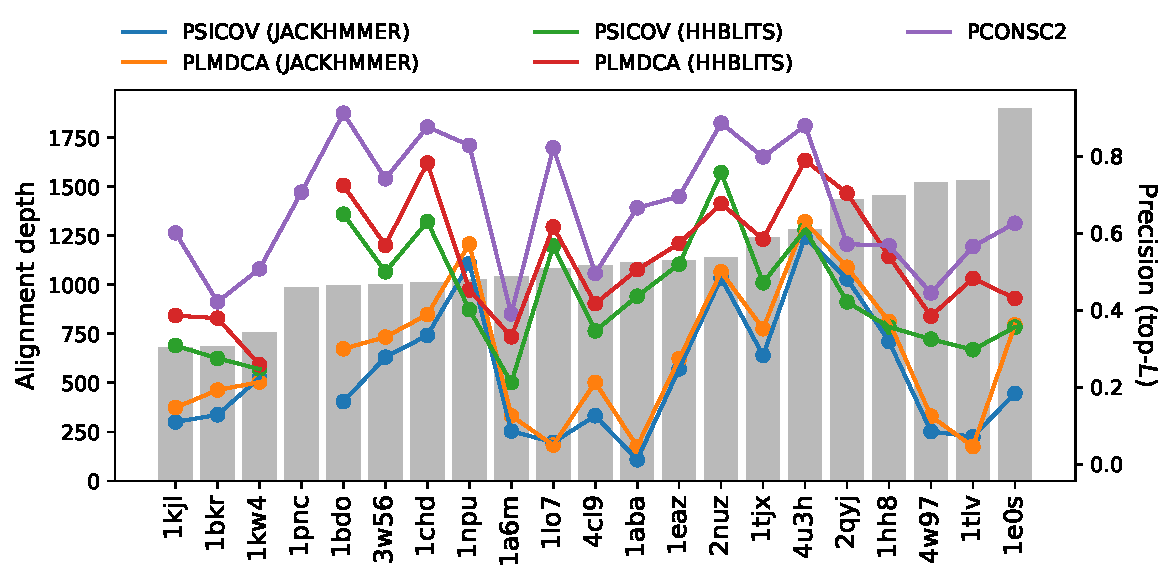
\includegraphics[width=\textwidth]{ample_proof_globpreccomp.pdf}
        \caption{}
        \label{fig:ample_proof_globpreccomp}
    \end{subfigure}
    
    \begin{subfigure}[b]{\textwidth}
        \centering
        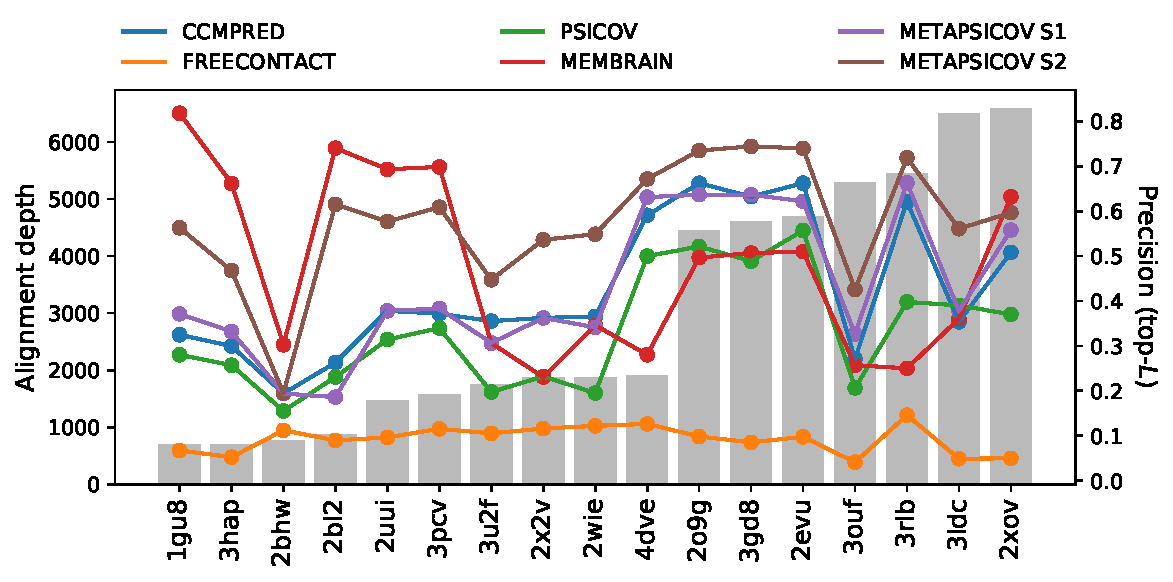
\includegraphics[width=\textwidth]{ample_proof_tmpreccomp.pdf}
        \caption{}
        \label{fig:ample_proof_tmpreccomp}
    \end{subfigure}
    
    \caption[Alignment depth and contact precision analysis of all protein targets]{Alignment depth and contact precision analysis of (a) globular and (b) transmembrane protein targets. Contact predictions were obtained with several contact prediction algorithms. Precision scores were calculated for the top-$L$ contact pairs. JACKHMMER and HHBLITS alignments for PSICOV and PLMDCA contact predictions in (a) were obtained with E-value 10\textsuperscript{-4}.} 
    \label{fig:ample_proof_preccomp}
\end{figure}

The depth of \gls{msa}s obtained for each target sequence suggests that sufficient numbers of divergent homologous sequences were available. Across all globular targets, the minimum alignment depth was obtained for Galectin-3 domain (\gls{pdb} ID: 1kjl) with 679 effective sequences and the maximum for G-protein Arf6-GDP (\gls{pdb} ID: 1e0s) with 1,897 effective sequences (\cref{fig:ample_proof_globpreccomp}). The median alignment depth for all globular targets was over 1,000, which was beyond the often suggested threshold of 200 sequences \cite{Simkovic2017-xs}. The \gls{msa}s for all transmembrane protein targets also surpassed this threshold comfortably. The median alignment depth was much higher than for globular targets with 1,878 sequences (\cref{fig:ample_proof_tmpreccomp}). The minimum, which was obtained for Sensory rhodopsin II (\gls{pdb} ID: 1gu8), was 692 sequences and the maximum for the sequence of Rhomboid protease GLPG (\gls{pdb} ID: 2xov) is 6,583.

In coevolution-based contact prediction, the precision depends on alignment depth. Despite sufficient number of effective sequences across all targets, findings presented here suggested that some (meta-)predictors cannot fully utilise greater alignment depths to correct contact pairs (\cref{fig:ample_proof_preccomp}). 

PCONSC2 --- a metapredictor using eight starting alignments and two contact predictors --- outperformed its individual parts for almost all globular targets (\cref{fig:ample_proof_globpreccomp}). Although only four individual components are shown in \cref{fig:ample_proof_globpreccomp}, the pattern translated across all 16 individual predictions per target. Such results suggested that precision greatly depends on the tool used to identify and select homologous sequences for the \gls{msa}. A closer inspection of mean precision scores resulting from HHBLITS- and JACKHMMER-based alignments showed higher precision scores for top-$L$ contact pairs based on the former alignments (\cref{table:ample_proof_pconsc2}). Nevertheless, the Machine Learning approach in PCONSC2 to combine more and less precise individual predictions resulted in superior precision in the output (\cref{table:ample_proof_pconsc2}). No correlation was observed between alignment depth and precision for either individual predictors or the metapredictor PCONSC2 (\cref{fig:ample_proof_globpreccomp}). 

\begin{table}[H]
    \centering
    \caption[Raw conact prediction precision values of PCONSC2 predictions]{Summary of mean PCONSC2 raw contact prediction precision based on JACKHMMER and HHBLITS alignments and PSICOV, PLMDCA and PCONSC2 coevolution-based contact prediction.}
    \label{table:ample_proof_pconsc2}
    \begin{tabularx}{\textwidth}{b b s s s s}
        \hline
        \multicolumn{2}{c}{\textbf{Contact prediction}} & \multicolumn{4}{c}{\textbf{Alignment E-value cutoff}} \\
        \cline{3-6} & & $1^{0}$ & $1^{-4}$ & $1^{-10}$ & $1^{-40}$ \\ 

        \hline
        \multirow{2}{1em}{PSICOV} & JACKHMMER  & 0.240 & 0.239 & 0.213 & 0.167 \\
                                  & HHBLITS    & 0.439 & 0.435 & 0.354 & 0.209 \\
        \hline
        \multirow{2}{1em}{PLMDCA} & JACKHMMER  & 0.293 & 0.288 & 0.252 & 0.140 \\ 
                                  & HHBLITS    & 0.545 & 0.530 & 0.447 & 0.224 \\
        \hline
        \hline
        PCONSC2                   &            & \multicolumn{4}{c}{0.667}     \\
        \hline
    \end{tabularx}
\end{table}

Contacts for transmembrane protein targets in this study were predicted with the metapredictor METAPSICOV and the transmembrane-specific predictor MEMBRAIN.

METAPSICOV STAGE 1 and STAGE 2 predictions outperformed MEMBRAIN in nine and ten cases, respectively, whilst MEMBRAIN outperformed METAPSICOV for the rest (\cref{fig:ample_proof_tmpreccomp}). The METAPSICOV algorithm utilises the raw predictions by CCMPRED, FREECONTACT and PSICOV to generate its STAGE 1 and STAGE 2 predictions. METAPSICOV STAGE 1 predictions were near identical to CCMPRED, whereby 12 of 13 targets showed an absolute $\Delta_{precision}$ of less than 0.05 (\cref{fig:ample_proof_tmpreccomp}). This similarity did not propagate to METAPSICOV STAGE 2 predictions with only a single target showing such similar precision values (\cref{fig:ample_proof_tmpreccomp}). Amongst the three raw predictors used by METAPSICOV, FREECONTACT performed by far the worst with a mean precision of 0.09 across all transmembrane targets. PSICOV showed similar trend to CCMPRED when assessed by target, which resulted in a mean absolute $\Delta_{precision}$ of 0.10.

\begin{figure}[H]
    \centering
    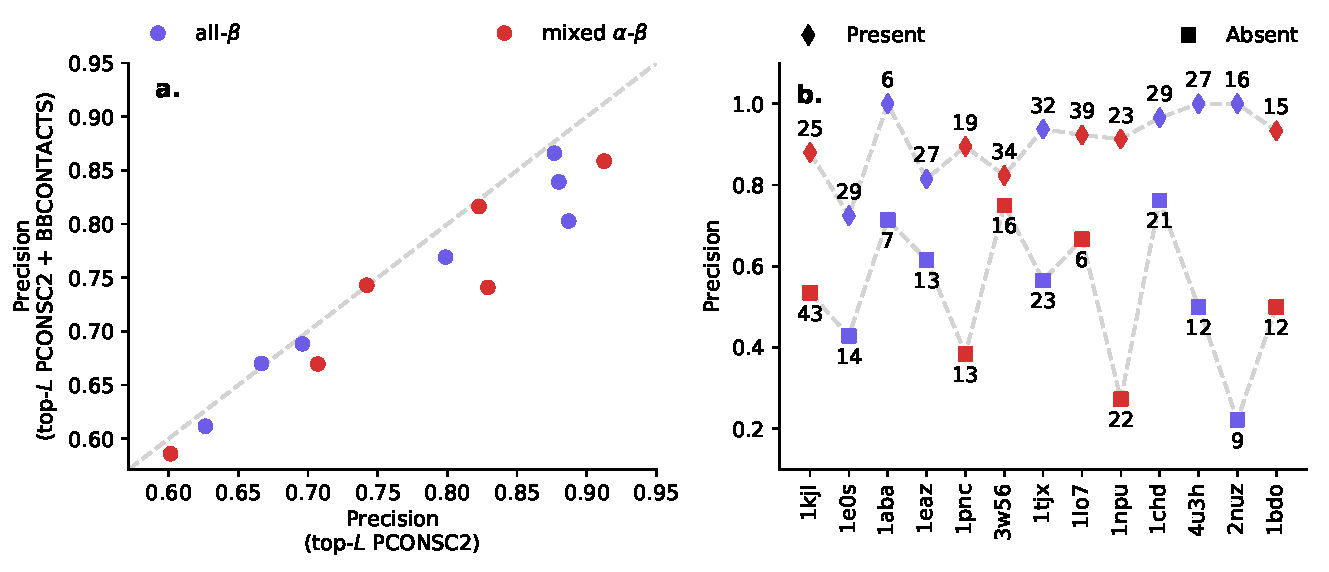
\includegraphics[width=\textwidth]{ample_proof_bbaddon.pdf}
    \caption[Evaluation of BBCONTACTS contact pairs]{Evaluation of predicted BBCONTACTS contact pairs. (a) Precision evaluation of PCONSC2 predicted contact map with and without BBCONTACTS. (b) Precision evaluation of BBCONTACTS contact pairs split by status of presence or absence in the base PCONSC2 contact list. Numbers besides each marker indicate the number of contacts. The rank order of scatter points is identical between both subplots and based on the PCONSC2 precision values (x-axis) in (a).}
    \label{fig:ample_proof_bbaddon}
\end{figure}

The addition of BBCONTACTS contact pairs to improve structure prediction accuracy for \textbeta-structure containing targets was a novel aspect introduced in this study. The initial step of the addition of BBCONTACTS contact pairs included the filtering of predicted one- and two-pair \textbeta-strand contacts from the original BBCONTACTS list (for further details, see \cref{sec:methods_bbcontacts_addition}). The findings in this study confirmed this for all \textbeta-structure containing targets. Precision values improved for all targets with changes ranging from 0.01 to 0.14 whilst retaining on average 80\% of all contacts. Filtered BBCONTACTS predicted contact maps were combined with other predicted contact maps, i.e. PCONSC2, to either upweight or add contact pairs. Findings in this study highlighted that upweighted contact pairs are more precise than ones to be added. The minimum precision score for a set of upweighted contacts was 0.72 for 29 contact pairs and the maximum of 1.00 for up to 27 contact pairs. In comparison, novel BBCONTACTS predicted contact pairs not present in the base predicted contact map ranged in precision scores from 0.22 (nine contacts) to 0.76 (21 contacts). 

Despite the high precision of predicted BBCONTACTS contact pairs, the merge of such pairs with top-$L$ PCONSC2 contact pairs resulted in an expected loss in precision for the resulting contact set (\cref{fig:ample_proof_bbaddon}). \Gls{tp} contacts, which dominate the predicted BBCONTACTS contact set, were also predicted by PCONSC2, and thus upweighted (\cref{fig:ample_proof_bbaddon}). Since upweighting does not affect the precision, the value remained unaffected after this procedure. However, contact pairs only predicted by BBCONTACTS contain more \gls{fp} contacts. Once added to the base PCONSC2 contact list, these contacts therefore reduced the precision value (\cref{fig:ample_proof_bbaddon}). Either subset of BBCONTACTS contacts did not show any correlation between the number it contained and its precision. The fold of the target did not show any clear distinction between better and worse sets of contacts either (\cref{fig:ample_proof_bbaddon}).

\subsection{Protein structure prediction} \label{subsec:ample_proof_strupred}
Predicted contact information is particularly useful to limit the conformation search space in \textit{ab initio} protein structure prediction \cite{Lee2017-oc}. Since such predictions are the basis for AMPLE studies presented in this thesis, it is important to analyse the improvement in decoy quality.

\begin{figure}[H]
    \centering
    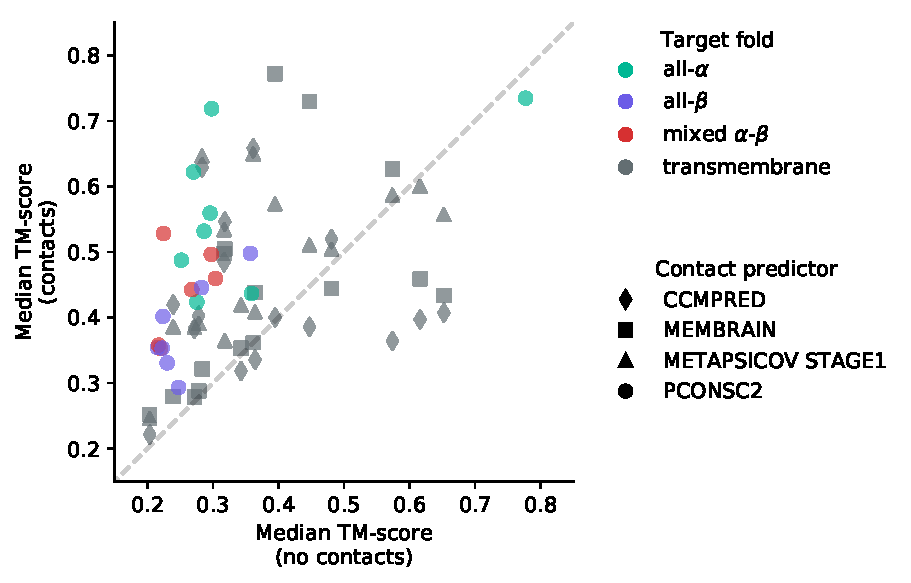
\includegraphics[width=\textwidth]{ample_proof_comproscon.pdf}
    \caption[Effect of contact distance restraints on \textit{ab initio} decoy quality]{Effect of contact distance restraints on \textit{ab initio} decoy quality by comparison of unrestrained (\textit{no contacts}) and contact-restrained (\textit{contacts}) median TM-scores for 1,000 decoys per target. Colours indicate the target fold and symbols the contact prediction algorithm.}
    \label{fig:ample_proof_comproscon}
\end{figure}

Globular protein targets benefited greatly from the addition of PCONSC2 contact predictions. All but one target saw median \gls{tmscore} improvements of at least 0.05 when comparing contact-assisted PCONSC2 decoys with simple ROSETTA decoys (\cref{fig:ample_proof_comproscon}). The greatest improvement over 1,000 decoys was achieved for Oxy-myoglobin (\gls{pdb} ID: 1a6m) with an improvement in median \gls{tmscore} of 0.42.  The decoys for Ankyrin (\gls{pdb} ID: 2qyj) showed a minor decrease in median \gls{tmscore} of 0.04; however, the median \gls{tmscore} for ROSETTA decoys was 0.78, and thus such minor decrease may be negligible. 

Previously, \textit{ab initio} protein structure prediction for globular targets was greatly limited by target fold and chain length. The addition of predicted residue-residue contacts enhanced decoy quality primarily for \textalpha-helical and mixed \textalpha-\textbeta\ protein targets (\cref{fig:ample_proof_globtmcomp}). Whilst only one all-\textalpha\ target had more than 50\% native-like decoys in its ROSETTA decoy set, five targets surpassed this threshold when PCONSC2 contact data was used to restrain the folding procedure. Similarly, the median \gls{tmscore} of no mixed \textalpha-\textbeta\ target decoy set surpassed the \gls{tmscore} threshold of 0.5 with ROSETTA decoys compared to one for PCONSC2 decoys with three further ones greater than 0.4. All-\textbeta\ targets also benefited from the addition of predicted contact restraints, although decoy set quality did not surpass the native-like threshold in terms of their median \gls{tmscore} (\cref{fig:ample_proof_globtmcomp}). Larger targets did not benefit any more than smaller targets from the addition of residue contacts to the structure prediction protocol. The only real exception to this were the decoys for the CheB methylesterase domain (\gls{pdb} ID: 1chd), for which the majority of ROSETTA decoys were almost random-like whilst PCONSC2 decoys are native-like (\cref{fig:ample_proof_globtmcomp}).

\begin{figure}[H]
    \centering
    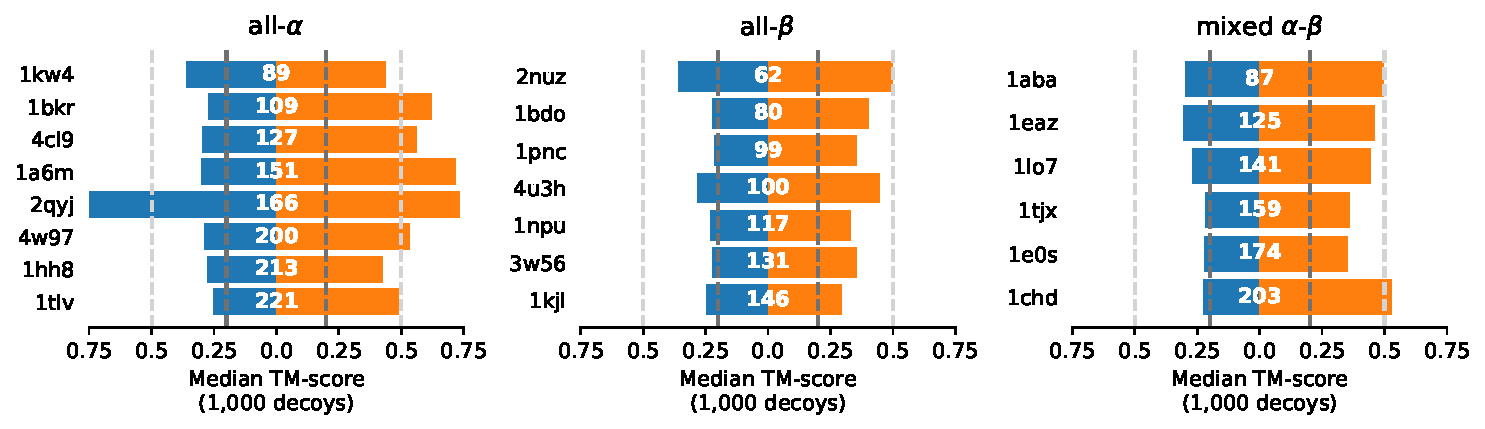
\includegraphics[width=\textwidth]{ample_proof_globtmcomp.pdf}
    \caption[TM-score comparison for globular targets separated by fold]{\gls{tmscore} comparison for globular targets separated by fold and ordered by target chain length. Median \gls{tmscore}s for 1,000 decoys generated with simple ROSETTA (orange) or contact-assisted ROSETTA (blue) runs. Numbers in each row correspond to the target chain length. Bars surpassing the dark gray line indicate that the majority of structures are better than random, whilst the light gray line indicates that the majority of structures are native-like \cite{Xu2010-kr}.}
    \label{fig:ample_proof_globtmcomp}
\end{figure}

The enhancement of \textbeta-structure specific contact pairs was an important part of this study. In \cref{subsec:ample_proof_conpred}, the high precision of added BBCONTACTS contact predictions was demonstrated. Thus, the next essential step was to explore how the BBCONTACTS supplement enhanced or degraded decoy quality after ROSETTA \textit{ab initio} protein structure prediction. Given 13 \textbeta-structure containing targets, eight targets achieved better overall decoy quality with added BBCONTACTS (\cref{fig:ample_proof_comprosconbb}). The smallest improvement was observed for target 1e0s with 0.01 \gls{tmscore} units, whilst the largest for target 1eaz with 0.05 units. The remaining five targets --- \gls{pdb} IDs 1chd, 1bdo, 1npu, 4u3h and 1tjx --- saw decreases in median \gls{tmscore} up to 0.03 when BBCONTACTS contact pairs were added as restraints (\cref{fig:ample_proof_comprosconbb}). No clear difference between fold classes, i.e. mixed \textalpha-\textbeta\ or all-\textbeta\ targets, was observed, although mixed \textalpha-\textbeta\ targets did show slightly greater extremes (\cref{fig:ample_proof_comprosconbb}).

\begin{figure}[H]
    \centering
    \begin{subfigure}[b]{\textwidth}
        \centering
        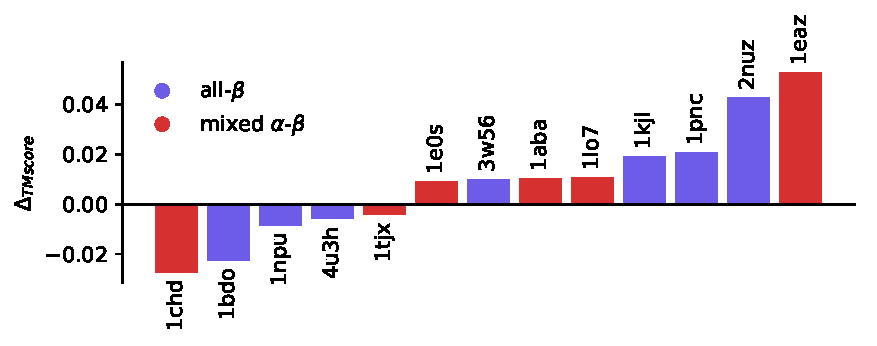
\includegraphics[width=\textwidth]{ample_proof_comprosconbb.pdf}
        \caption{}
        \label{fig:ample_proof_comprosconbb}
    \end{subfigure}
    
    \begin{subfigure}[b]{\textwidth}
        \centering
        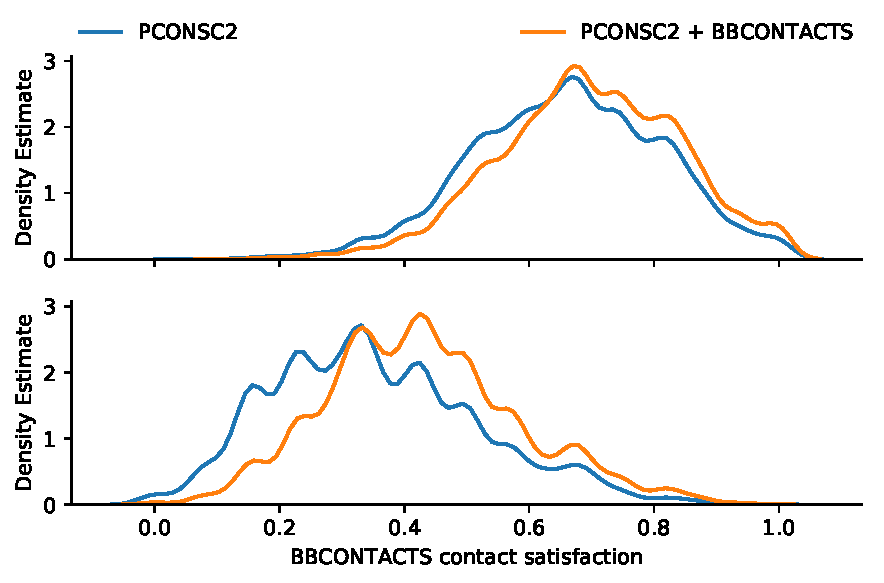
\includegraphics[width=\textwidth]{ample_proof_bbsat.pdf}
        \caption{}
        \label{fig:ample_proof_bbsat}
    \end{subfigure}
    
    \caption[Decoy analysis of effects of BBCONTACTS contact addition]{(a) \Gls{tmscore} comparison for \textbeta-structure containing globular targets separated by fold and ordered by the difference in median \gls{tmscore} between PCONSC2 and PCONSC2+BBCONTACTS decoys. Positive values indicate a better median \gls{tmscore} in favour of PCONSC2+BBCONTACTS decoys, whilst negative values those for PCONSC2. \Gls{pdb} IDs are provided alongside each bar. (b) Satisfaction of BBCONTACTS contact predictions in decoys with added \textbeta-structure contact restraints (PCONSC2 + BBCONTACTS) and those without (PCONSC2).}
\end{figure}

An analysis of the satisfaction of BBCONTACTS contact predictions in decoys where extra \textbeta-sheet contact pairs were used as restraints compared those where they were not highlighted a greater satisfaction in the former. This indicates that the added and upweighted BBCONTACTS \textbeta-structure contact restraints enhanced the formation of \textbeta-sheets in the resulting decoys, which would explain the overall improved decoy quality for more than half the targets. A separation of contact satisfaction by upweighted and added BBCONTACTS contact pairs indicated that the upweighting had less effect compared to the addition (\cref{fig:ample_proof_bbsat}). Although the former shows a marginal improvement in BBCONTACTS contact satisfaction of decoys without upweighted restraints, the difference was minimal. In comparison, PCONSC2 decoys without the added BBCONTACTS restraints showed less satisfaction for such contacts, indicating that they did not form as often compared to PCONSC2+BBCONTACTS. In combination with the upweighting, these resulted showed that \textbeta-rich regions are predicted more accurately when BBCONTACTS contact pairs supplement PCONSC2 contacts.

Transmembrane protein targets were modelled using residue-residue contact predictions derived with CCMPRED, MEMBRAIN and METAPSICOV STAGE1. A ROSETTA benchmark was also run to compare contact-assisted decoys to the current norm. Findings in this study highlighted the much improved decoy quality for almost all targets when predicted contact information was used to reduce the conformational sampling space (\cref{fig:ample_proof_comproscon}). Across all methods, only the decoys for ATP synthase subunit C (\gls{pdb} ID: 2wie) suffered from the addition of contact restraints during \textit{ab initio} protein structure prediction. ROSETTA generated decoys with median \gls{tmscore} of greater than 0.6 when no contact restraints were used. This contrasts strongly with contact-assisted decoy sets, for which only METAPSICOV STAGE1 predictions yielded overall native-like decoys, i.e. median TM-score of greater than 0.5. 

A split for decoy quality comparison between no-contact and contact-assisted decoy sets by contact prediction algorithm showed that CCMPRED contact predictions were not sufficiently precise to always improve decoy quality. Four out of 13 targets are predicted more accurately without CCMPRED contact information (\cref{fig:ample_proof_tmtmcomp}). In comparison, MEMBRAIN and METAPSICOV STAGE1 contact predictions resulted in enhanced decoy quality to the extend that only one decoy set was worse than their no-contact counterpart (\cref{fig:ample_proof_tmtmcomp}). Most notably, either of the three contact predictions per target performed better for certain targets. The most extreme example may be the decoy sets for Bacteriorhodopsin (\gls{pdb} ID: 3hap) for which CCMPRED contacts resulted in decoy quality degradation of 0.06, METAPSICOV STAGE1 in a slight improvement of 0.06 and MEMBRAIN in an improvement of 0.28 \gls{tmscore} units. This translated into absolute decoy counts with native-like fold --- i.e., \gls{tmscore} $\geq 0.5$ --- of the following: 274 for decoys without contact guidance, 289 for CCMPRED contact guidance, 538 for METAPSICOV STAGE1 contact guidance, and 996 for MEMBRAIN contact guidance. Similar examples exist (e.g., \gls{pdb} IDs 1gu8, 3rlb or 4dve in \cref{fig:ample_proof_tmtmcomp}) and highlight that no single method yielded the best decoys under all circumstances.

\begin{figure}[H]
    \centering
    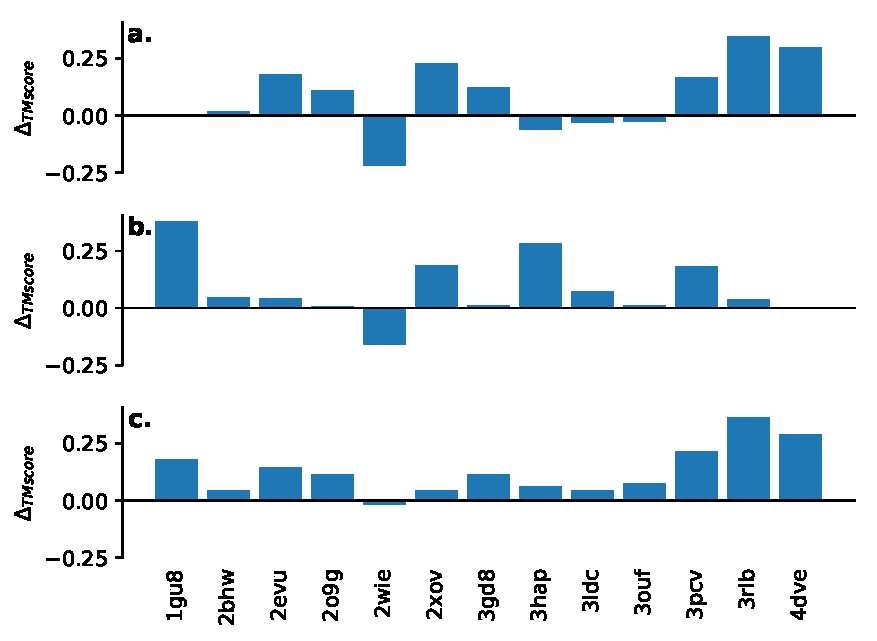
\includegraphics[width=\textwidth]{ample_proof_tmtmcomp.pdf}
    \caption[TM-score difference between contact-assisted and simple decoys]{TM-score difference between contact-assisted and simple ROSETTA decoys for transmembrane protein targets. Positive $\Delta_{TMscore}$ values indicate more accurate contact-assisted decoys, whilst negative values better decoys without the addition of contacts. $\Delta_{TMscore}$ values were computed by median \gls{tmscore}. Contact restraints were obtained with (a.) CCMPRED, (b.) MEMBRAIN, and (c.) METAPSICOV STAGE1.}
    \label{fig:ample_proof_tmtmcomp}
\end{figure}

\subsection{Molecular Replacement}
The most important aspect of this study was the impact of contact-assisted decoys in AMPLE-\gls{mr}. Contact-unassisted AMPLE is primarily limited by a target's chain length and fold, which typically cannot exceed 150 residues, and performs poorly for \textbeta-rich folds \cite{Bibby2012-lm}. Findings presented in \cref{subsec:ample_proof_strupred} outlined improvements in overall decoy quality when predicted contact information was used as distance restraints in \textit{ab initio} protein structure prediction. However, it is yet to be seen how the improved decoy quality translates into \gls{mr} structure solutions.

\subsubsection{Globular protein targets} \label{subsec:ample_proof_globmr}
Structure solutions were attempted for a total of 21 globular targets. Simple ROSETTA decoys --- those without contact restraints and AMPLE's current default --- resulted in nine structure solutions (\cref{fig:ample_proof_mrglob}). The addition of PCONSC2 contact-restraints to the structure prediction procedure improved decoy quality to achieve four additional structure solutions. However, the structure of the N-terminal region of P67Phox (\gls{pdb} ID: 1hh8) was not solved when PCONSC2-restrained decoys were used compared to simple ROSETTA ones. The addition of BBCONTACTS distance restraints to upweight and supplement PCONSC2 contacts enabled a further unique solution for the Phosphoinositol (3,4)-bisphosphate PH domain (\gls{pdb} ID: 1eaz) (\cref{fig:ample_proof_mrglob}).

\begin{figure}[H]
    \centering
    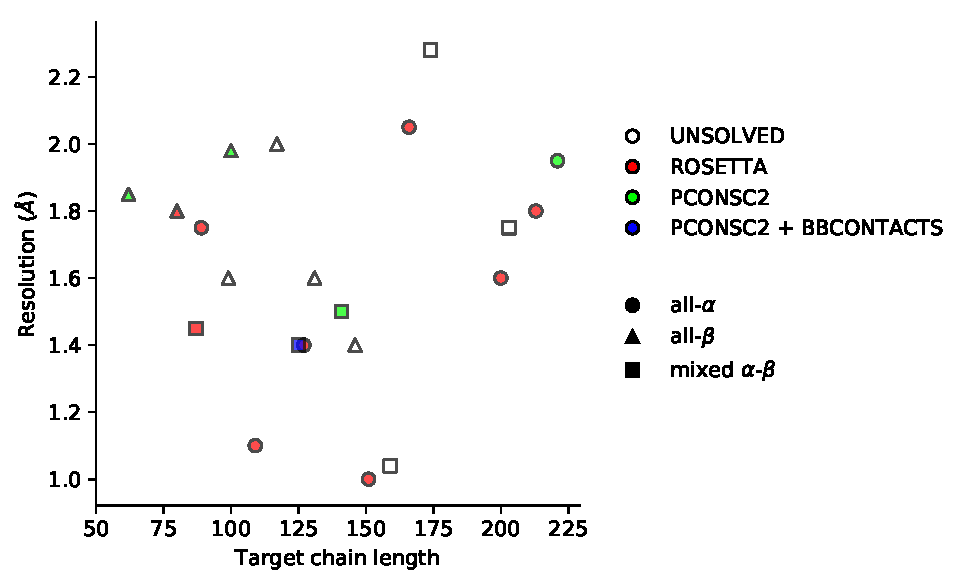
\includegraphics[width=\textwidth]{ample_proof_mrglob.pdf}
    \caption[Structure solution summary for globular targets]{Summary of structure solutions obtained with AMPLE using no-contact ROSETTA, PCONSC2-contact-restraint-assisted ROSETTA and PCONSC2 + BBCONTACTS-assisted ROSETTA decoy sets. Empty markers indicate unsolved targets. Filled markers highlight the minimum decoy set by complexity of the prediction procedure to obtain \gls{mr} structure solution. Marker shape distinguishes the fold class.}
    \label{fig:ample_proof_mrglob}
\end{figure}

The majority of structure solutions were obtained for all-\textalpha\ targets in the dataset, with a total of eight structure solutions (\cref{fig:ample_proof_mrglob}). Seven of those eight structure solutions were achieved with unrestrained ROSETTA decoys, with target chain lengths up to 213 residues. The largest target in the globular dataset, and the only all-\textalpha\ target that required residue contacts, totals 221 residues in target chain length, which exceeded AMPLE's previously benchmarked limits for globular targets greatly \cite{Bibby2012-lm}. In comparison to all-\textalpha\ targets, \textbeta-structure containing proteins required predicted contact restraints to result in sufficiently accurate decoys for \gls{mr}. Across all-\textbeta\ and mixed \textalpha-\textbeta\ targets, only two structure solutions were obtained with unrestrained ROSETTA decoys. This contrasts to an additional three targets when PCONSC2 restraints were used during \textit{ab initio} structure prediction. Furthermore, the addition of BBCONTACTS contact restraints enabled an additional structure solution, yielding much greater success for \textbeta-structure containing protein targets compared to the previous default. Structure solutions for \textbeta-containing targets were obtained for target chain lengths up to 141 residues (\cref{fig:ample_proof_mrglob}).

Two exceptional cases specifically exemplified the application of contact predictions and their benefit to \gls{mr}. The first example were the structure solutions for 4-hydroxybenzoyl CoA thioesterase (\gls{pdb} ID: 1lo7), which were based on AMPLE ensemble search models derived from the PCONSC2 and PCONSC2+BBCONTACTS decoy sets. Without contact restraints, AMPLE search models did not accurately represent the target fold (\cref{fig:ample_proof_1lo7_rosetta}). In comparison, precise residue-residue contact predictions primarily restraining the large \textbeta-sheet yielded decoys of sufficient quality to achieve \gls{mr} structure solution with both PCONSC2 (\cref{fig:ample_proof_1lo7_pconsc2}) and PCONSC2+BBCONTACTS (\cref{fig:ample_proof_1lo7_pconsc2bbcontacts}) decoy sets.

\begin{figure}[H]
    \centering
    \begin{subfigure}[b]{0.32\textwidth}
        \centering
        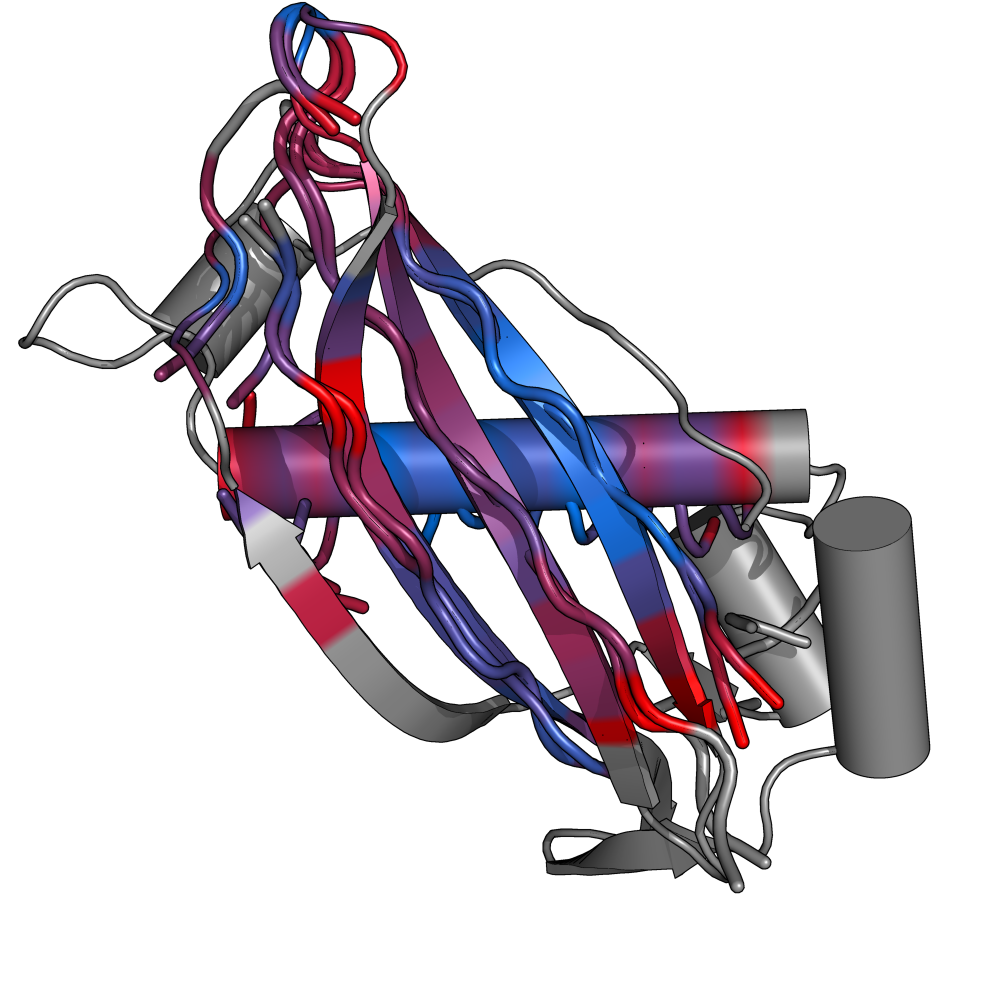
\includegraphics[width=\textwidth]{ample_proof_1lo7_rosetta_c1_tl50_r3_polyAla.png}
        \caption{}
        \label{fig:ample_proof_1lo7_rosetta}
    \end{subfigure}
    %
    \begin{subfigure}[b]{0.32\textwidth}
        \centering
        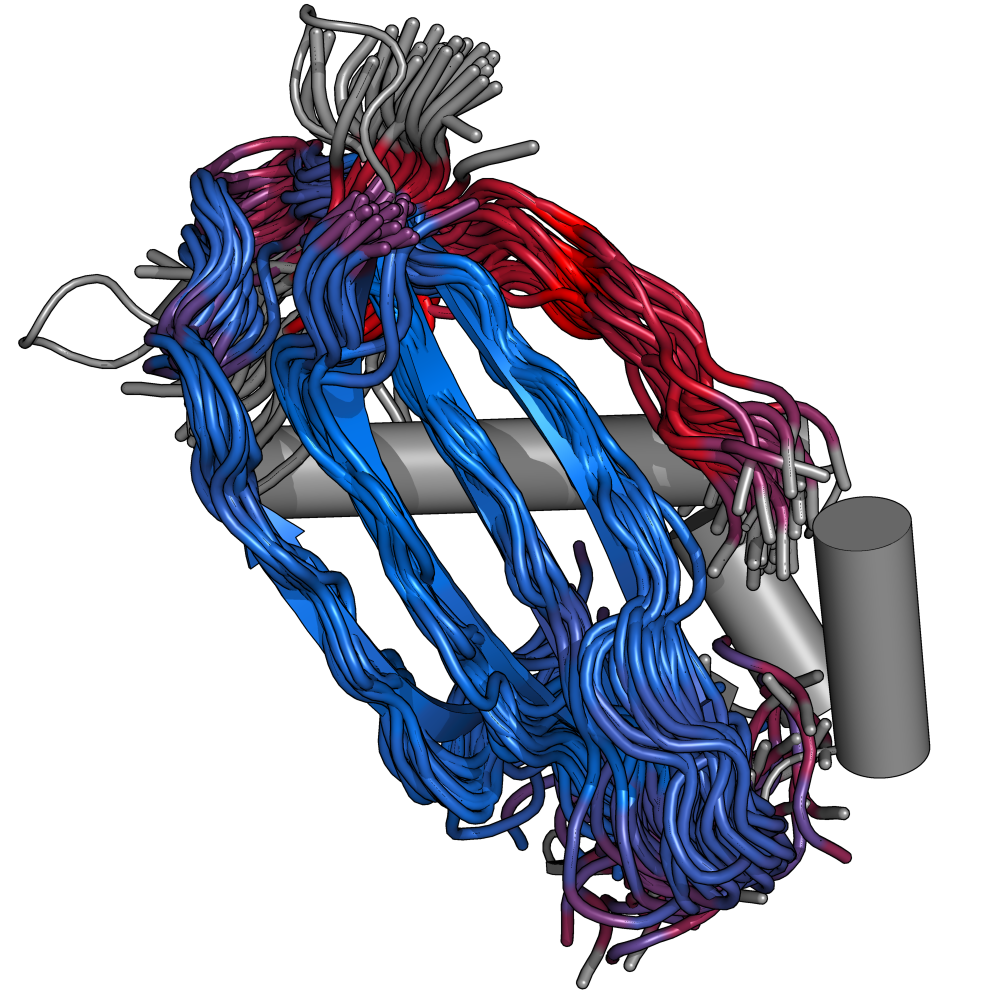
\includegraphics[width=\textwidth]{ample_proof_1lo7_pconsc2_c2_tl55_r3_reliable.png}
        \caption{}
        \label{fig:ample_proof_1lo7_pconsc2}
    \end{subfigure}
    % 
    \begin{subfigure}[b]{0.32\textwidth}
        \centering
        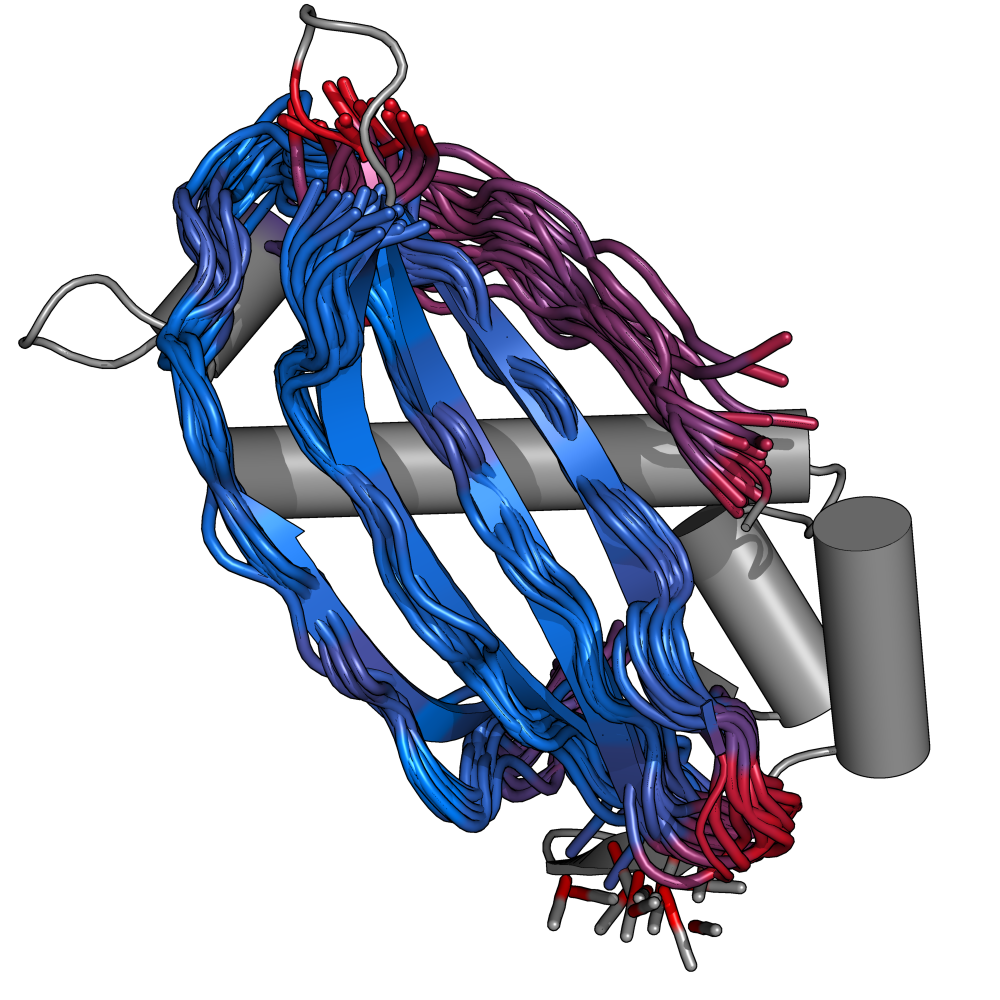
\includegraphics[width=\textwidth]{ample_proof_1lo7_pconsc2bbcontacts_c3_tl50_r2_reliable.png}
        \caption{}
        \label{fig:ample_proof_1lo7_pconsc2bbcontacts}
    \end{subfigure}

    \caption[Structural superposition of three search models for target 1lo7]{Structural superposition of the (a) ROSETTA (C\textalpha\ \gls{rmsd} 2.814 \AA; ensemble contains two structures), (b) PCONSC2 (C\textalpha\ \gls{rmsd} 1.748 \AA; 30 members) and (c) PCONSC2+BBCONTACTS (C\textalpha\ \gls{rmsd} 1.760 \AA; 15 members) search-model ensembles for 4-hydroxybenzoyl CoA thioesterase (\gls{pdb} ID: 1lo7). Examples are the highest scoring search models based on SHELXE \gls{cc} score, with only (b) and (c) leading to successful \gls{mr} structure solutions. Search models are shown as tubes and crystal structures as cartoons. (a) and (c) are 50\% of the target sequence, while (b) is 55\%. The colour scale illustrates the pairwise C\textalpha\ \gls{rmsd} between each search-model ensemble (represented by its first member) and the crystal structure, with blue representing the minimum C\textalpha\ \gls{rmsd} and red the maximum. Unaligned residues are coloured grey.}
    \label{fig:ample_proof_example_1lo7}
\end{figure}

The second exceptional case, \gls{pdb} ID 1e0s, did not yield any \gls{mr} structure solution with either decoy set according to the stringent criteria for \gls{mr} success applied in this study (see \cref{sec:methods_mr_success}). However, a \gls{rio} analysis of PHASER solutions, i.e. after \gls{mr}, indicated that some PCONSC2 and PCONSC2+BBCONTACTS AMPLE search models were placed partially correctly (\cref{fig:ample_proof_example_1e0s}). For the top PCONSC2 search model, 40\% (12 residues) of the search model residues were correctly superimposed, albeit out of register on the target structure (PHASER \gls{tfz}=4.7, PHASER \gls{llg}=16) (\cref{fig:ample_proof_1e0s_pconsc2}). For the top PCONSC2+BBCONTACTS search model, 77\% (30 residues) of the search model were superimposed in an in-register fashion (PHASER \gls{tfz}=5.3, PHASER \gls{llg}=17) (\cref{fig:ample_proof_1e0s_pconsc2bbcontacts}). For the latter, expert manual intervention might allow structure determination, but in this case the correct solution was not prominent in the list of \gls{mr} placements. Nevertheless, it is clear that even when overall structure solution was not automatically achieved the PCONSC2+BBCONTACTS search model provided better results which might be recoverable as successes in the future as \gls{mr} and post-\gls{mr} software improves still further.

\begin{figure}[H]
    \centering
    \begin{subfigure}[b]{0.48\textwidth}
        \centering
        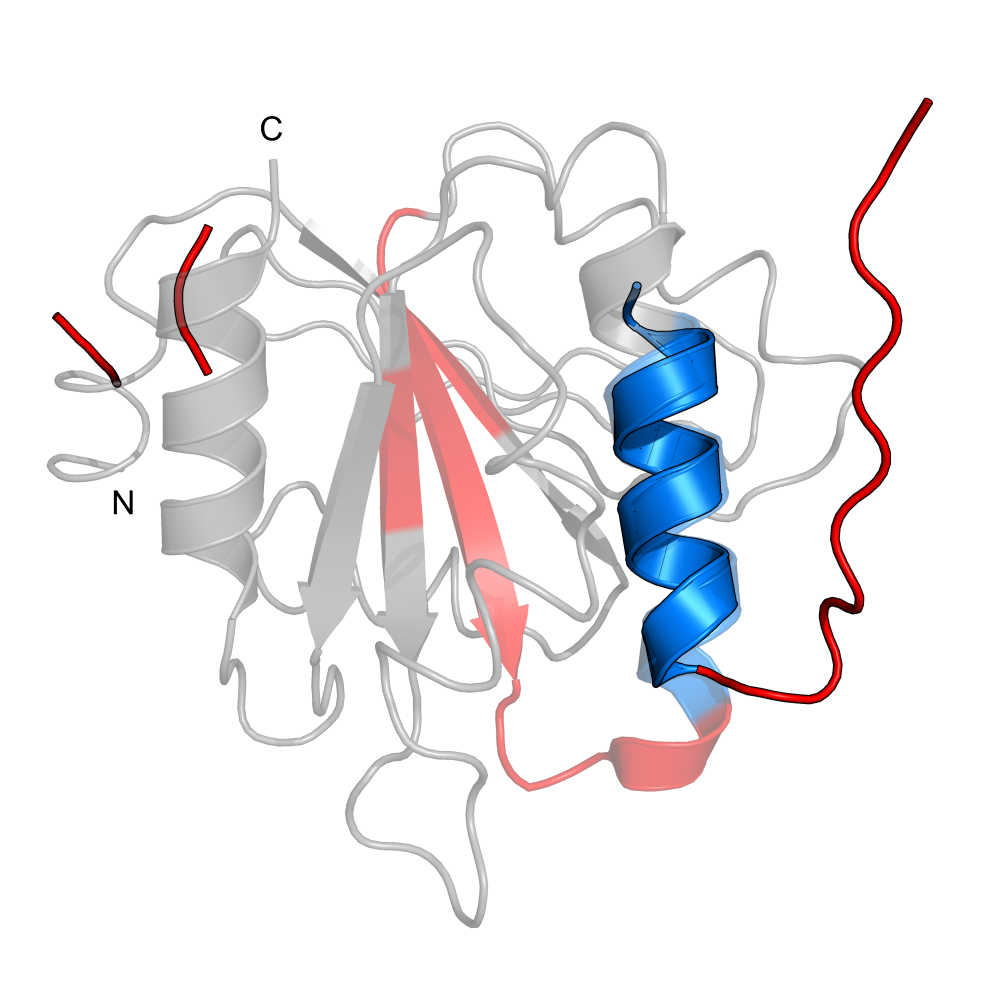
\includegraphics[width=\textwidth]{ample_proof_1e0s_pconsc2.png}
        \caption{}
        \label{fig:ample_proof_1e0s_pconsc2}
    \end{subfigure}
    %
    \begin{subfigure}[b]{0.48\textwidth}
        \centering
        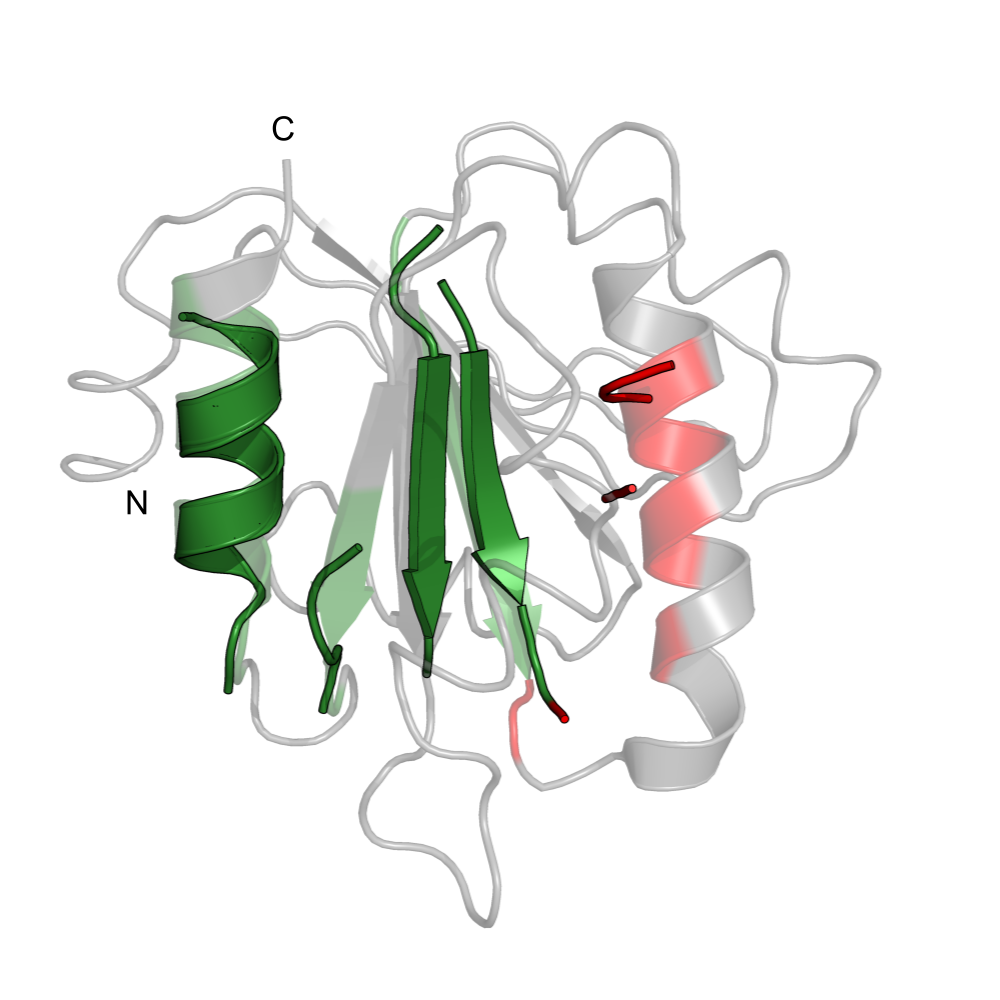
\includegraphics[width=\textwidth]{ample_proof_1e0s_pconsc2bbcontacts.png}
        \caption{}
        \label{fig:ample_proof_1e0s_pconsc2bbcontacts}
    \end{subfigure}

    \caption[Top-PHASER solutions for target 1e0s]{Top-PHASER solutions for \gls{pdb} ID 1e0s based on \gls{rio} scores for (a) PCONSC2 (\gls{rio} score 12) and (b) PCONSC2+BBCONTACTS (\gls{rio} score 30) search models. Search-model colour coding indicates useful superposition of residues by in- (green) or out-of-sequence register (blue) residues as well as misplaced (red) residues. The addition of BBCONTACTS restraints produced a more accurate model with correctly placed \textbeta-strands that was placed correctly. Both structures are shown in cartoon representation with the crystal structure shown as a transparent cartoon. Unaligned reference crystal structure residues are coloured grey.}
    \label{fig:ample_proof_example_1e0s}
\end{figure}

With much improved decoy quality deriving from the use of predicted contact restraints to guide \textit{ab initio} structure prediction, the question arose whether AMPLE's existing cluster-and-truncate approach remained the most suitable for obtaining a conserved, native-like core from the decoys found in the largest clusters. For globular targets solved using simple ROSETTA decoys, certain features throughout AMPLE's cluster-and-truncate approach typically correlated with eventual success in structure solution \cite{Bibby2012-lm}. In general, the greater the number of decoys in the largest cluster the more likely the success was with derived search models. Truncation removed structurally variant parts leading to smaller more accurate ensemble subsets of the cluster decoys. Although successful search models were found at every truncation interval, the majority were derived with search models containing around 30 residues. Lastly, each of the potential nine search models derived at each truncation level (three subclustering radii with three side chain treatments each) can lead to non-redundant structure solutions. Similar observations, particularly with respect to the most successful search model size range were made for other target classes \cite{Thomas2017-sh,Thomas2015-wu} and for \textit{ab initio} decoys made with QUARK \cite{Keegan2015-zb}.

A size comparison of the largest clusters of ROSETTA and PCONSC2+BBCONTACTS (or PCONSC2 for all-\textalpha) decoys indicated a median increase of 122 decoys per cluster in the latter. All cluster sizes increased except for target 2qyj. More accurate \textit{ab initio} decoys are directly linked to larger cluster sizes because of the associated increase in convergence \cite{Simons1997-oe}. Here, as expected, the largest cluster contains better than average quality decoys but the size of the largest cluster does not link to the total number of successful search models.  

\begin{figure}[H]
    \centering
    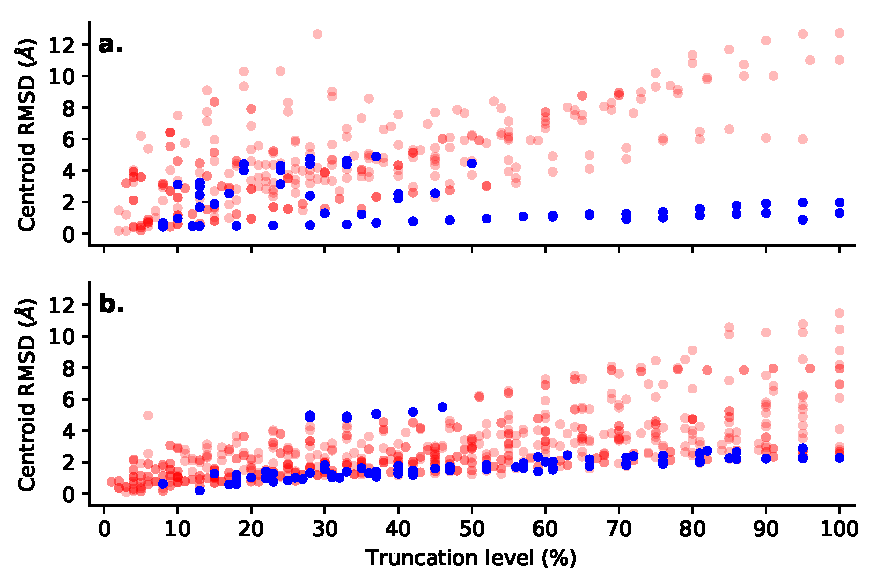
\includegraphics[width=\textwidth]{ample_proof_mrglobtl.pdf}
    \caption[Effect of progressive truncation on RMSD of ensemble centroid]{The percentage of sequence in the search model is mapped against the \gls{rmsd} over all C\textalpha\ atoms of the first representative of each search-model ensemble derived from the largest cluster against the native structure. Successful structure solutions of individual search models are highlighted in blue and unsuccessful solutions in red.  Progressively darker shades of either colour correspond to increasing numbers of overlapping points.  Progressive truncation is shown for (a) ROSETTA and (b) PCONSC2+BBCONTACTS decoys (or PCONSC2 decoys for all-\textalpha\ targets).}
    \label{fig:ample_proof_mrglobtl}
\end{figure}

In comparison to the clustering step, the progressive truncation of decoys in the largest cluster at 20 different intervals directly affects the number of successful search models. An analysis of the progressive truncation and the effects on search model accuracy revealed that all successful search model ensembles had a C\textalpha-\gls{rmsd} better than 5.5\AA\ compared to the native structure (\cref{fig:ample_proof_mrglobtl}). Although the latter cutoff is independent of whether predicted contact information was provided during \textit{ab initio} modelling, a clear difference between the ROSETTA and PCONSC2+BBCONTACTS (or PCONSC2 for all-\textalpha) ensemble search models for all targets can be observed. In total, ROSETTA decoys for all targets produced 1,314 ensemble search models based on the largest clusters. In comparison, PCONSC2+BBCONTACTS decoys generated for the same targets 2,469 search model ensembles from the largest clusters. This increase is the result of a more successful subclustering process due to the increased structural homogeneity across the decoys in the largest cluster. The most notable difference between the two sets is detected for the Small G-protein ARF6-GDP (\gls{pdb} ID: 1e0s), which produced three ensemble search models based on ROSETTA decoys and 90 based on PCONSC2+BBCONTACTS decoys. Additionally, ensemble search models with structural fragments of 15-40 residues of the target sequence are more likely to succeed in \gls{mr} phasing than larger or smaller search models \cite{Bibby2012-lm}. Here we find that the same range is most successful for contact-assisted decoys (\cref{fig:ample_proof_mrglobcompl}). Out of 246 successful search models for PCONSC2+BBCONTACTS decoys derived from the largest cluster (PCONSC2 for all-\textalpha), 101 successful search models contained 15-40 residues. Significantly, some cases like the PH domain of TAPP1 (\gls{pdb} ID: 1eaz) and the N-terminal bromodomain of human BRD4 (\gls{pdb} ID: 4cl9) only solved with truncated search models in this size range. Nevertheless, structure solutions were also achieved with larger or smaller search models. The smallest search model leading to a structure solution contained nine residues (8\% of total sequence) and solved the Calponin Homology domain from human \textbeta-spectrin (\gls{pdb} ID: 1bkr). In comparison, the largest successful search model in terms of residues was found for the designed full consensus ankyrin (\gls{pdb} ID: 2qyj) domain with 158 residues (95\% of total), and in terms of percentage of the total sequence the untruncated, 62 residue search model for \textalpha-spectrin SH3 domain (\gls{pdb} ID: 2nuz) was successful. Therefore, although truncating the \textit{ab initio} decoys at different levels remains essential for contact-assisted decoys, biasing sampling into the most successful size range may be advantageous in future runs.

The truncated decoys are further processed by subclustering at three different atomic radii, with the resulting subclusters previously found to be similarly successful \cite{Bibby2012-lm}. Similar trends are seen here: 36\% of structure solutions with ROSETTA decoys were achieved with a subclustering radius of 1\AA, 36\% at a radius of 2\AA, and 28\% at a radius of 3\AA. For PCONSC2+BBCONTACTS (or PCONSC2 for all-\textalpha) decoy sets similar numbers were observed (35\% at radius of 1\AA; 40\% at 2\AA; 25\% at 3\AA). Nevertheless, in terms of number of targets solved all three subclustering radii were essential. Largest-cluster decoys for target 1eaz produced a total of 327 search models, but only one solved and this derived from a subclustering radius of 1\AA. In comparison, contact-assisted decoys from the largest cluster for target 4u3h achieved structure solutions solely with decoys subclustered at 2\AA. A single search model with subclustering radius of 3\AA\ solved the target 4cl9 with ROSETTA decoys. The final step in search model creation is the side-chain processing of each subclustered ensemble. Similarly to the subclustering, no difference was observed between ROSETTA and PCONSC2+BBCONTACTS decoys. For both the polyalanine treatment is most successful, covering 37\% of successful search models for ROSETTA decoys and 44\% for PCONSC2+BBCONTACTS decoys. For almost all targets, the polyalanine side-chain treatment would be enough to obtain a structure solution.  However, some cases, like the target 1eaz, only solve with either or both of the remaining treatments.  Thus, relying solely on polyalanine side-chain treatment may limit the overall success rate, although trialling polyalanine ensemble search models first might lead to structure solution faster.

\begin{figure}[H]
    \centering
    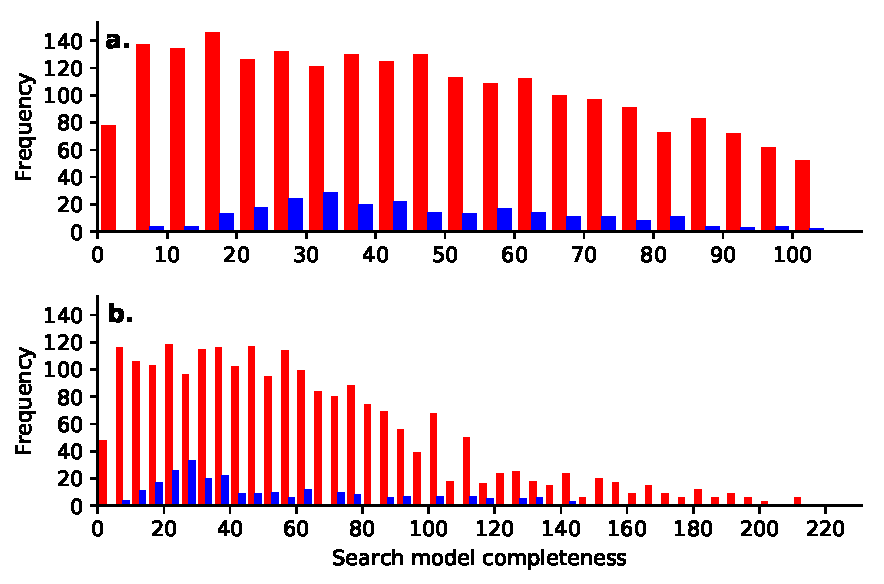
\includegraphics[width=\textwidth]{ample_proof_mrglobcompl.pdf}
    \caption[Summary of AMPLE truncation ranges for structure solution]{Summary of AMPLE truncation ranges for structure solution. (a) Percentage of residues and (b) number of residues per chain in search model mapped against the number of search models leading to structure solution (blue) or not (red).}
    \label{fig:ample_proof_mrglobcompl}
\end{figure}

\subsubsection{Transmembrane protein targets}
The \gls{mr} structure solution attempts given the decoy sets for transmembrane protein targets was conducted by Dr Jens Thomas and is documented in \textcite{Thomas2017-qu} and \textcite{Thomas2017-sh}.

In summary, \gls{mr} structure solution successes with decoys restrained by either of the three contact prediction protocols --- CCMPRED, MEMBRAIN and METAPSICOV STAGE1 --- were mixed. CCMPRED solved three targets, MEMBRAIN solved
five and METAPSICOV STAGE1 decoys solved four. Simple ROSETTA decoys resulted in four structure solutions. CCMPRED and METAPSICOV STAGE1 both solved target 4dve, which could not be solved with any other method, and METAPSICOV STAGE1 also solved target 2o9g, which had previously only been solved with the AMPLE library of ideal helices.

\section{Discussion}
The change in statistical model for residue-residue contact prediction has enabled great improvements to its precision. Today, predicted contact information is often used to restrain the conformational search space to enable accurate \textit{ab initio} protein structure prediction. In this study, the effect of such improved structure predictions was examined with a particular interest of their application in unconventional \gls{mr} in AMPLE. The main focus of the presented work rested with the aim to extend AMPLE's target tractability, both for larger and more \textbeta-rich protein targets.

The addition of predicted residue-residue contacts unsurprisingly improved the quality of \textit{ab initio} protein structure predictions, which is in line with numerous other studies \cite[e.g.,][]{Marks2011-os,Michel2014-eg,Kosciolek2014-bt,Ovchinnikov2015-tn,Ovchinnikov2016-jj,Michel2017-xh,De_Oliveira2018-sg,Ovchinnikov2017-nd,Wang2017-rx,Dos_Santos2018-lq}. The improved decoy quality directly translated to further structure solutions with AMPLE. Contact-unassisted decoys, i.e. the current default, achieved nine and four solutions for globular and transmembrane protein targets, respectively. In comparison, contact-assisted decoys solved a further five globular targets, whilst contact-assisted decoys solved some different targets compared to contact-unassisted decoys for transmembrane protein targets.

The initial findings in this study highlighted the successful application of contact prediction to extend the target tractability with regards to the target chain length. \textcite{Bibby2012-lm} previously benchmarked \textit{ab initio} protein structure predictions up to chain lengths of 120 residues. However, the findings indicated that larger targets should be tractable with AMPLE, especially all-\textalpha\ ones \cite{Bibby2012-lm}. The results in this study confirmed such extended target tractability, with contact-unassisted decoys leading to structure solutions up to 213 residues for globular targets and 223 residues for transmembrane protein targets. The addition of contacts to limit the conformational search space enabled structure solutions for the largest target in the globular target dataset with a 221-residue chain length and the transmembrane dataset with a 249-residue chain length. The fact that both of these targets are the largest in their sets is highly suggestive that contact-assisted decoys may enable solutions for much larger targets. In fact, recent research highlighted the successful \textit{ab initio} structure prediction of globular and transmembrane protein targets with target chain lengths in excess of 300 residues \cite{Ovchinnikov2017-nd}, which further supports this claim.

AMPLE was previously also limited by the target fold \cite{Bibby2012-lm}. Whilst the majority of all-\textalpha\ protein targets were comfortably tractable, mixed \textalpha-\textbeta\ and all-\textbeta\ targets were not \cite{Bibby2012-lm}. This limitation primarily arose from upstream limitations in \textit{ab initio} protein structure prediction but also the challenging task of tracing \textbeta-sheets in SHELXE, which was used to assess the successful structure solution. The use of contact-assisted decoys in AMPLE improved the target tractability for \textbeta-structure-containing protein targets. Structure solutions for four additional, \textbeta-structure-containing targets were obtained when contact-assisted decoys were used. A novel approach of combining \textbeta-sheet-specific contact pairings with a normal base prediction enabled the structure solution of one further target. Although no \gls{mr} structure solutions were lost when BBCONTACTS contact pairs were added to a base set of contact restraints, further studies are required to support routine application in AMPLE. Furthermore, BBCONTACTS contact pairs were identified by analysis of a CCMPRED predicted contact map, which is generally much noisier than metapredictor alternatives. Thus, further studies may explore the benefits or drawbacks of BBCONTACTS based on alternative predicted contact maps. Lastly, since the release of BBCONTACTS, other \textbeta-strand specific contact identification protocols have been developed \cite{Mao2018-mo}, which may need to be explored too.

Beyond the proof-of-concept study outlined in this chapter, it is very important to appreciate new limitations and unexplored areas of this work. At the time of conducting this study, PCONSC2 proved to be the state-of-the-art metapredictor. However, numerous alternatives have since been developed with more advanced Machine Learning architectures to post-process multiple individual contact predictions \cite[e.g.,][]{Jones2015-vq,Ovchinnikov2015-tn}. Furthermore, the optimal introduction of contacts as distance restraints into \textit{ab initio} protein structure prediction protocols is not yet clearly defined, and thus leaves the choice to the user without much comparison or guidance as to which works best. Lastly, contact information was exclusively used to restrain the \textit{ab initio} protein structure prediction procedure despite other potential applications in the AMPLE cluster-and-truncate algorithm. Subsequent chapters therefore explore additional uses of contact information for obtaining more accurate structure predictions (\cref{chap:rosetta_energy_functions}), identifying the implications on different structure prediction protocols (\cref{chap:alternate_abinitio_protocols}), and establishing improved decoy selection for better AMPLE processing (\cref{chap:ample_decoys}).


\chapter{Evaluation of ROSETTA distance-restraint energy functions on contact-guided \textit{ab initio} structure prediction} \label{chap:rosetta_energy_functions}
\clearpage
% \section{Introduction}
The extended tractability of the AMPLE program for globular and transmembrane protein targets through the use of residue-residue contact predictions to restrain \textit{ab initio} structure prediction was highlighted in \cref{chap:proof_of_principle}. However, the study explored exclusively the metapredictor PCONSC2 for globular targets without considering any alternatives. It thus served solely as proof of principle for applications of contact predictions in unconventional \gls{mr}.

Besides the individual contact prediction algorithms employed by the PCONSC2 protocol, numerous metapredictors have been developed exploiting different combinations of starting alignments and individual contact predictors to identify the strongest correlating pairs for optimal contact prediction \cite{Kamisetty2013-le,Skwark2014-qp,Jones2015-vq,Ma2015-vo,He2017-fn,Michel2017-pm,Wang2017-rx}. Furthermore, each of those protocols typically includes its own post-prediction algorithms to find a consensus amongst individual predictions and/or further identify patterns characteristic for residue pairings between secondary structure elements in a protein fold. Thus, depending on the overall protocol, the resulting predictions may differ significantly despite the same underlying algorithms to generate starting alignments and to predict residue contact pairs.

Furthermore, the precision of contact predictions used as distance restraints in \textit{ab initio} structure prediction improves the accuracy of the folding process significantly. However, a diversity of structure prediction protocols, whether fragment-based or not, have been applied and each with a unique integration of contact information as distance restraints \cite{Marks2011-os,Michel2014-eg,Adhikari2015-lb,Jones2015-vq,Ovchinnikov2015-tn,Adhikari2018-lj}. Such divergence results in three major problems: (1) researchers cannot directly compare results, and thus have to test each protocol against their own with every newly published approach; (2) novice users might find it difficult to make appropriate decisions given the diversity of algorithms and lack of comparative studies; and (3) users only interested in the information encoded in predicted contact pairs are at risk of picking the most readily available approach over the most accurate for their problem.

Thus, the presented work was aimed at extensively comparing state-of-the-art contact prediction and \textit{ab initio} protein structure prediction protocols with a focus on the use of such resulting decoys in unconventional \gls{mr}, with a particular focus on AMPLE users.

\section{Materials \& Methods}
\subsection{Target selection of PREDICTORS dataset} \label{sec:methods_dataset_predictors}
This study was conducted using 18 out of 27 targets in the PREDICTORS dataset (\cref{sec:methods_dataset_predictors}). All nine targets with PFAM alignment depths of less than 100 were excluded (\cref{table:appendix_dataset_predictors}).

\subsection{Contact prediction}
Residue contacts for each target sequence were predicted using three different metapredictors, namely METAPSICOV \cite{Jones2015-vq}, GREMLIN \cite{Kamisetty2013-le}, and PCONSC2 \cite{Skwark2014-qp}. Web servers for METAPSICOV v2016-02 (\url{http://bioinf.cs.ucl.ac.uk/METAPSICOV}) and GREMLIN v2015-12 (\url{http://gremlin.bakerlab.org}) were used to retrieve two sets of contact predictions. Web servers were preferred in this study over local installations to best imitate the typical behaviour of AMPLE users. Both servers were used with default settings.

The GREMLIN web server returns the raw contact prediction files as well as pre-formatted ROSETTA distance restraints. The raw contact prediction files were downloaded to allow different contact selection thresholds as well as local conversion into ROSETTA restraints files. The METAPSICOV web server returned two contact prediction files, one after STAGE1 and another after STAGE2 post-prediction processing. In this study, contact predictions after STAGE1 (referred to as METAPSICOV from here onwards) were chosen. The PCONSC2 contact prediction set was obtained using a local installation of PCONSC2 due to downtime of the web server at the time of this study. The settings and databases were identical to \cref{sec:ample_proof_conpred}. Additionally to the three main contact predictions outlined above, a set of BBCONTACTS restraints was obtained for protein targets containing \textbeta-strands (\cref{sec:methods_bbcontacts_addition}).

The sequence-database versions of all three metapredictors, whether on- or offline, were identical to those outlined in \cref{sec:ample_proof_methods}.

\subsection{Contact-to-restraint conversion} \label{subsec:ample_predicotrs_con2res}
Contact restraints for \textit{ab initio} protein structure prediction were generated by selecting the top-ranking contact pairs from each prediction and reformatting them into a ROSETTA-readable format. The number of top-ranking contact pairs varied according to the two energy functions used (FADE cutoff: \textit{L}; SIGMOID cutoff: 3\textit{L}/2; where \textit{L} corresponds to the number of residues in the protein chain). Both energy functions are sigmoidal functions and introduced into the ROSETTA folding protocol in the same fashion. 

Neither energy function enforces a specified distance between restrained atoms but reward those that meet it. The two energy functions (\cref{fig:ample_predictors_efuncs}) differ in that the FADE function does not only have an upper but also a lower bound. Based on previous findings \cite{Michel2014-eg, Skwark2014-qp}, the FADE function was set to acknowledge a formed restraint if the participating C\textbeta\ atoms (C\textalpha\ in case of Gly) were within 9\AA. In comparison, the SIGMOID function was defined with amino acid specific distances for C\textbeta\ atoms (C\textalpha\ in case of Gly) to recognise the different sizes of each amino acid \cite{Kamisetty2013-le, Ovchinnikov2015-tn}.

\begin{figure}[H]
    \centering
    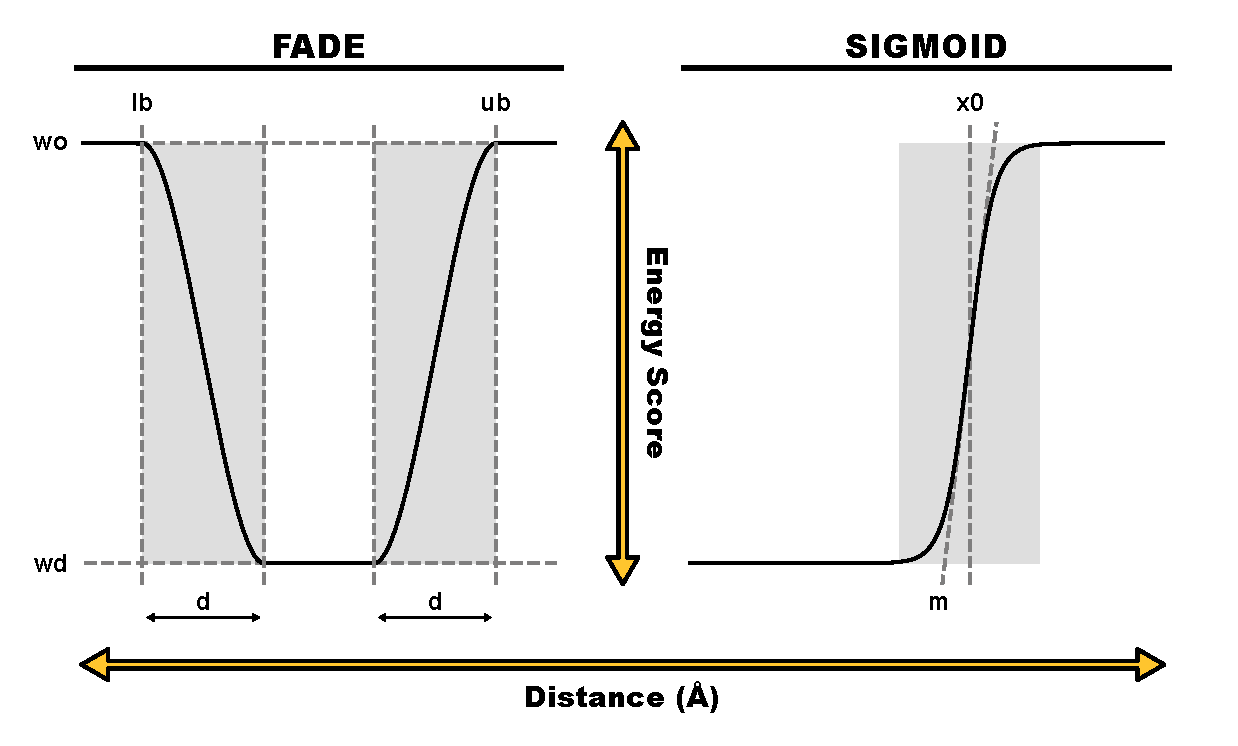
\includegraphics[width=\textwidth]{ample_predictors_efuncs.pdf}
    \caption[Schematic comparison of ROSETTA energy functions]{Schematic comparison of two ROSETTA energy functions. Abbreviations corresponds to input parameters.}
    \label{fig:ample_predictors_efuncs}
\end{figure}

To explore the effects of the varying ROSETTA energy function definitions, six separate contact restraint lists were created for each \textalpha-helical target and nine for each \textbeta-structure containing target. The top-ranking contact pairs per prediction were converted using the PCONSFOLD definition of the FADE function \cite{Michel2014-eg}, the GREMLIN definition of the SIGMOID function \cite{Ovchinnikov2015-tn}, and additionally the PCONSC2+BBCONTACTS definition of the FADE function for \textbeta-structure containing targets (\cref{sec:bbcontacts_addition}).

The conversion was handled in AMPLE and invoked with the keywords outlined in \cref{table:ample_predictors_kwargs}. The \texttt{-restraints\_factor} keyword defines the factor used to select contact pairs based on the target chain length, i.e. a factor of 1.5 would correspond to 3\textit{L}/2 contact pairs. The \texttt{-distance\_to\_neighbour} keyword defines the minimum distance in sequence space between contact pair participating residues, which were set to 5 residues for the FADE function \cite{Michel2014-eg} and 3 for the SIGMOID function \cite{Ovchinnikov2015-tn}. Additionally, all distance restraints were given an additional weight when introduced via the SIGMOID energy function to balance its energy term with all remaining terms in the ROSETTA scoring function (Sergey Ovchinnikov, personal communication). This was achieved by using the \texttt{-restraints\_weight} keyword and weights of 1.0 and 3.0 for the FADE and SIGMOID energy functions.

The addition of BBCONTACTS to existing sets of contacts was achieved with the FADE function in an identical manner as described in \cref{sec:bbcontacts_addition}. In comparison, the \texttt{SCALARWEIGHTED} term in the GREMLIN implementation of the SIGMOID energy function \cite{Ovchinnikov2015-tn} was multiplied by the number of occurrences of each contact pair in the combined map.

\begin{table}[H]
    \centering
    \caption[AMPLE keyword arguments for two ROSETTA energy functions]{AMPLE keyword arguments for FADE and SIGMOID ROSETTA energy functions.}
    \label{table:ample_predictors_kwargs}
    \begin{tabularx}{\textwidth}{ s b }
        \hline
        \textbf{Energy Function} & \textbf{AMPLE keywords} \\
        \hline
        \multirow{6}{1em}{FADE} & \texttt{-contact\_file <FILENAME>} \\
                                & \texttt{-contact\_format <FORMAT>} \\
                                & \texttt{-energy\_function FADE} \\
                                & \texttt{-restraints\_factor 1.0} \\
                                & \texttt{-distance\_to\_neighbour 5} \\
                                & \texttt{-restraints\_weight 1.0} \\
        \hline
        \multirow{6}{1em}{FADE (BBCONTACTS)} & \texttt{-contact\_file <FILENAME>} \\
                                & \texttt{-contact\_format <FORMAT>} \\
                                & \texttt{-energy\_function FADE} \\
                                & \texttt{-restraints\_factor 1.0} \\
                                & \texttt{-distance\_to\_neighbour 5} \\
                                & \texttt{-restraints\_weight 1.0} \\
        \hline
        \multirow{6}{1em}{SIGMOID} & \texttt{-contact\_file <FILENAME>} \\
                                & \texttt{-contact\_format <FORMAT>} \\
                                & \texttt{-energy\_function SIGMOID} \\
                                & \texttt{-restraints\_factor 1.5} \\
                                & \texttt{-distance\_to\_neighbour 3} \\
                                & \texttt{-restraints\_weight 3.0} \\
        \hline
        \multirow{6}{1em}{SIGMOID (BBCONTACTS)} & \texttt{-contact\_file <FILENAME>} \\
                                & \texttt{-contact\_format <FORMAT>} \\
                                & \texttt{-energy\_function SIGMOID\_bbcontacts} \\
                                & \texttt{-restraints\_factor 1.5} \\
                                & \texttt{-distance\_to\_neighbour 3} \\
                                & \texttt{-restraints\_weight 3.0} \\
        \hline
    \end{tabularx}
\end{table}

\subsection{\textit{Ab initio} protein structure prediction}
Six or nine individual lists of contact restraints generated for each target were used in separate ROSETTA \textit{ab initio} protein structure prediction runs. Additionally, protein structures were predicted without any predicted contact restraints to acquire a control decoy set. Homologous fragments were excluded during fragment library generation to imitate the folding process of a target with unknown fold. Fragment libraries were generated for each target using a local installation of ROSETTA v2015.22.57859. PSIPRED secondary structure predictions were included from contact prediction runs and provided via the \texttt{-psipredfile} option. In total, 1,000 \textit{ab initio} decoys were generated per run using ROSETTA v2015.22.57859 with default settings \cite{Rohl2004-dj} and one of the seven or ten (six/nine plus control) contact conditions described in \cref{subsec:ample_predicotrs_con2res}. In total, 162 sets of models were generated across 18 protein targets.

\subsection{Molecular Replacement}
Besides considering decoy quality, one key interest of this study was the assessment of the decoy sets created in the previous step as \textit{ab initio} \gls{mr} search model templates. To reduce the enormous computational cost linked to trialling 162 decoy sets, 108 sets were chosen from the following conditions: simple ROSETTA, PCONSC2 prediction and FADE function, GREMLIN prediction and SIGMOID function, METAPSICOV prediction and FADE function, and where applicable, PCONSC2+BBCONTACTS, GREMLIN+BBCONTACTS and METAPSICOV+BBCONTACTS predictions and FADE function. Overall, this resulted in four \gls{mr} runs for the six \textalpha-helical targets, seven runs for the six all-\textbeta, and seven runs for the six mixed \textalpha-\textbeta\ targets. The resulting 108 model sets were trialled in AMPLE v1.1.0 and CCP4 v7.0.28. Structure solution success was assessed as described in \cref{sec:methods_mr_success}.

\section{Results}
\subsection{Direct comparison of three contact metapredictors}
In this study, a direct comparison between three metapredictors --- GREMLIN, METAPSICOV and PCONSC2 --- was carried out. Residue-residue contact pairs were predicted for 18 protein target sequences with a range of chain lengths and numbers of effective sequences in their PFAM \gls{msa}s.

METAPSICOV was the most precise contact predictor across the protein target dataset in this study (\cref{fig:ample_predictors_cutoff}). The difference between the three metapredictors was most evident in the highest-scoring contact pairs (\textit{L}/10). The median precision values for METAPSICOV and PCONSC2 contact predictions were above 50\% up to \textit{L} contact pairs. GREMLIN, in comparison, predicted contacts with a median precision score at least 20\% worse than that of METAPSICOV and 15\% worse than PCONSC2. However, at 3\textit{L}/2 contact pairs the median precision scores were much more similar across the three different metapredictors: METAPSICOV and PCONSC2 were near identical, and GREMLIN is at most 12\% worse compared to the other two. Inspecting the mean precision scores over a continuous range of selection cutoff values illustrated further the difference between METAPSICOV, PCONSC2 and GREMLIN (Fig \ref{fig:ample_predictors_covprc}). The former two similarly high precision scores compared to the average precision scores for GREMLIN, which were approximately 0.2 precision score units lower. Added to the difference in precision scores was the difference in sequence coverage (\cref{fig:ample_predictors_covprc}). Although producing the on-average worst contact predictions out of the three metapredictors, GREMLIN contact predictions had the highest sequence coverage. However, an analysis of singleton contact pairs, usually with high degrees of \gls{fp} predicted contacts, revealed a positive correlation ($\rho_{Pearson}=0.47$; $p<0.001$) between the fraction of singleton contact pairs and sequence coverage and hinted to a weak negative correlation ($\rho_{Pearson}=-0.27$; $p<0.05$) between the fraction of singleton contact pairs and contact precision (\cref{fig:ample_predictors_singletons}).

\begin{figure}[H]
    \centering
    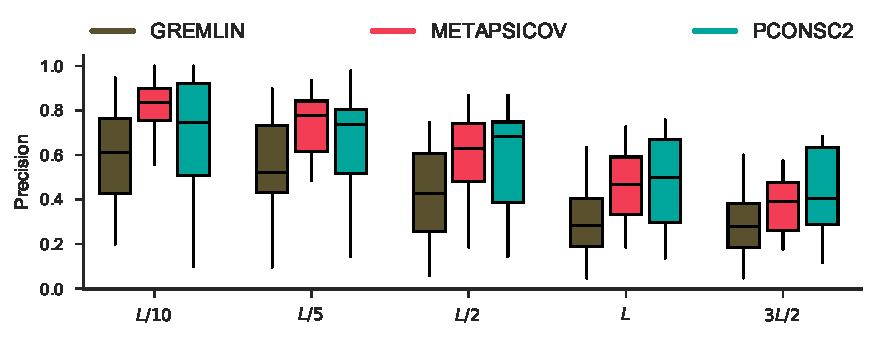
\includegraphics[width=\textwidth]{ample_predictors_cutoff.pdf}
    \caption[Precision analysis of three metapredictors]{Distribution of precision values for three metapredictors computed at five contact selection cutoff values relative to the target chain length (\textit{L}).}
    \label{fig:ample_predictors_cutoff}
\end{figure}

\begin{figure}[H]
    \centering
    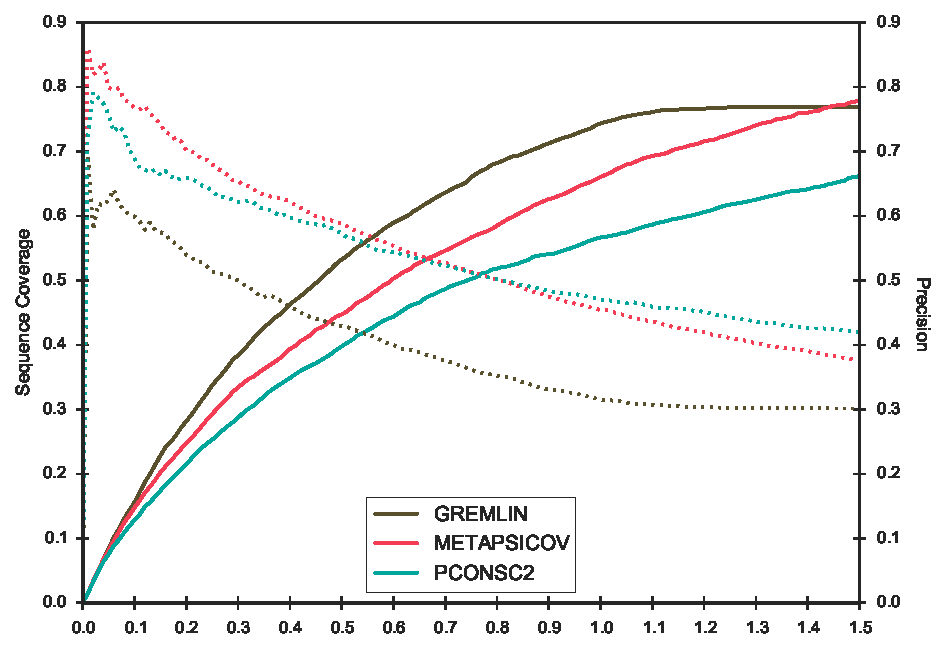
\includegraphics[width=\textwidth]{ample_predictors_covprc.pdf}
    \caption[Sequence coverage and contact precision analysis]{Average sequence coverage (line) and contact prediction precision scores (dashed) across a continuous range of contact selection cutoffs ranging from $[0.0, 1.5]$ for all targets.}
    \label{fig:ample_predictors_covprc}
\end{figure}

\begin{figure}[H]
    \centering
    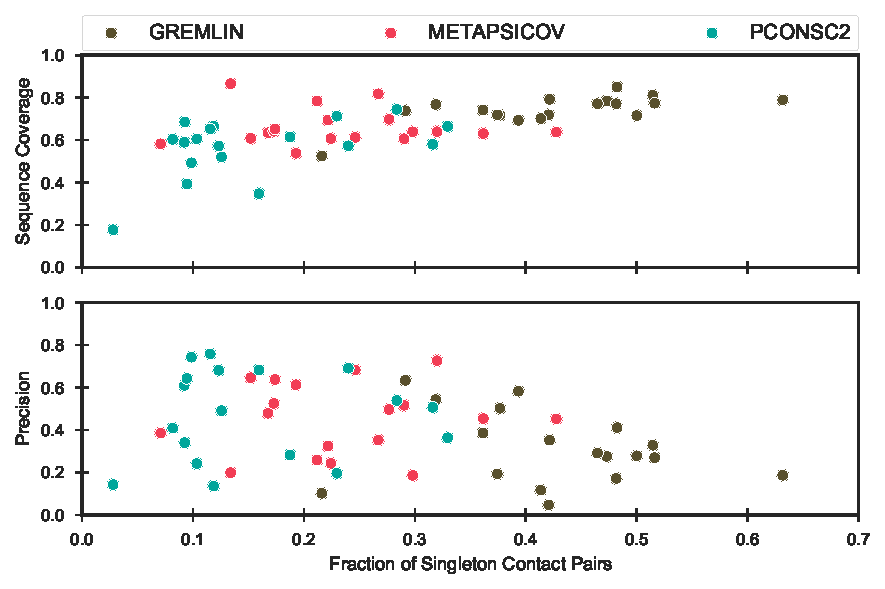
\includegraphics[width=\textwidth]{ample_predictors_singletons.pdf}
    \caption[Contact singleton analysis for three metapredictors]{Contact singleton analysis compared against the precision of top-\textit{L} contact pair lists for three metapredictors.}
    \label{fig:ample_predictors_singletons}
\end{figure}

Given that the overall precision of contact pairs predicted by the three metapredictors differed, it was important to understand where the difference originated. To investigate this, a comparison of the precision values at different cutoff levels on a per-target basis was performed. For the majority of targets the precision scores were very similar across the three metapredictors (\cref{fig:ample_predictors_prcpeaks}). However, the prediction precision of some targets differed significantly. For example, the METAPSICOV prediction for the human retinoic acid nuclear receptor HRAR (\gls{pdb}: 1fcy) contained high precision in its highest scoring (top-\textit{L}/10) contact pairs (\cref{fig:ample_predictors_prcpeaks}). In comparison, GREMLIN and PCONSC2 predictions for the same target contained less precise contact pairs (\textDelta \textsubscript{METAPSICOV-GREMLIN} $L/10=-0.522$; \textDelta \textsubscript{METAPSICOV-PCONSC2} $L/10=-0.435$). However, the addition of further contact pairs up to 3\textit{L}/2 resulted in near-identical precision across the three metapredictors for this target. A second example illustrating such a difference were the contact predictions for the human galectin-3 CRD sequence (\gls{pdb}: 4lbj). In contrast to the previous example, the data showed high precision scores for the METAPSICOV and PCONSC2 predictions for this target, yet low precision for the top GREMLIN contact pairs (\textDelta \textsubscript{METAPSICOV-GREMLIN} $L/10=-0.231$; \textDelta \textsubscript{METAPSICOV-PCONSC2} $L/10=0.077$). 

\begin{figure}[H]
    \centering
    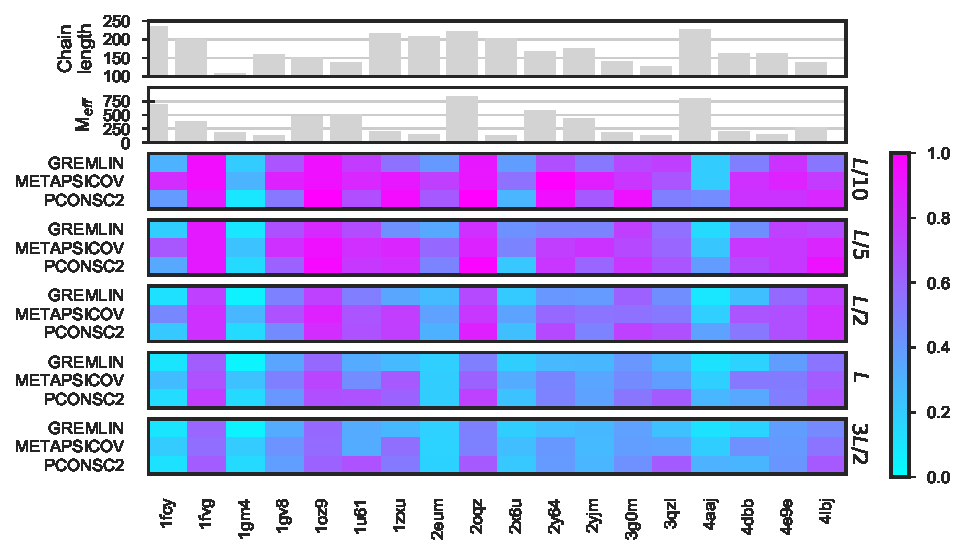
\includegraphics[width=\textwidth]{ample_predictors_prcpeaks.pdf}
    \caption[Comparison of contact precision for three metapredictors]{Contact prediction precision scores from three metapredictors for 18 targets at different contact pair selection thresholds (\textit{L}, which is the target chain length). The PFAM alignment depth is given by means of \gls{meff}. The colour scale corresponds to the precision in range $[0, 1]$.}
    \label{fig:ample_predictors_prcpeaks}
\end{figure}

The data presented in \cref{fig:ample_predictors_prcpeaks} also indicated that there was no direct link between chain length or \gls{meff} and the precision of the resulting contact predictions. The N-(5'-phosphoribosyl)anthranilate isomerase sequence (\gls{pdb}: 4aaj) with a chain length of 228 residues and 750 effective sequences in its PFAM \gls{msa} yielded a mean precision at \textit{L}/10 contact pairs of 0.283 (top-\textit{L}: 0.195) across the three metapredictors. This strongly contrasted with the sequence of sortase B (\gls{pdb}: 2oqz), which showed similar characteristics yet obtained  mean precision at \textit{L}/10 contact pairs of 0.938 (top-\textit{L}: 0.622).

Although the contact predictions differed in precision, an interesting question rested with the similarity of the predicted contact pairs amongst the sets. Thus, the similarity of contact predictions across the three metapredictors was an important metric to evaluate the most appropriate algorithm for AMPLE users. Using the Jaccard similarity index to evaluate the direct overlap of contact pairs across sets of predictions, the data suggested very little similarity between the contact predictions of the three metapredictors for each target (\cref{fig:ample_predictors_jaccardidx}). As with the differences in precision scores at higher cutoff thresholds, the Jaccard index was also lower --- indicating less overlap --- at higher cutoff thresholds. However, it is worth noting that the Jaccard index only considers identical matches and did not consider the neighbourhood of a contact pair. Thus, the index does not highlight similar regions with contact pairs in both maps.

\begin{figure}[H]
    \centering
    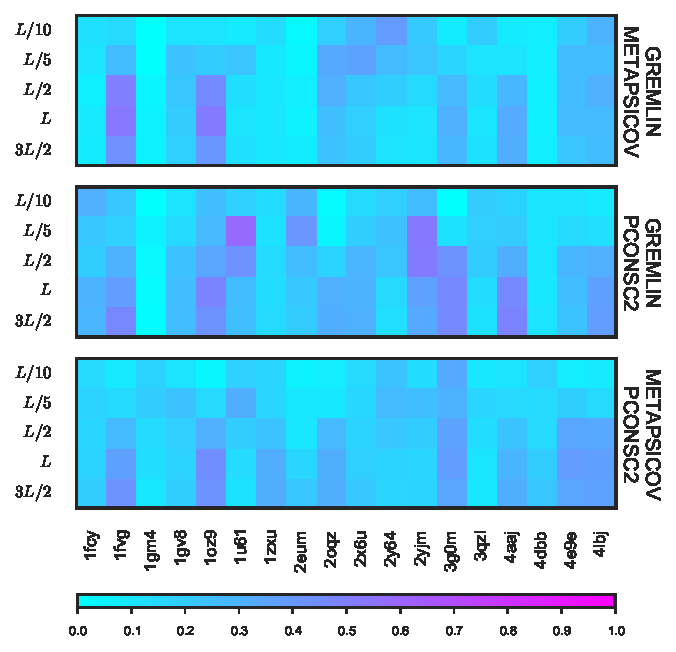
\includegraphics[width=0.8\textwidth]{ample_predictors_jaccardidx.pdf}
    \caption[Metapredictor contact pair similarity analysis]{Jaccard similarity index illustrates a higher degree of overlap between metapredictor contact predictions with increasing numbers of contact pairs included in the calculation. The three panels show the different comparisons. The color scale corresponds to the Jaccard index in range $[0, 1]$.}
    \label{fig:ample_predictors_jaccardidx}
\end{figure}

\subsection{Protein structure prediction with two ROSETTA energy functions}
The accuracy of the starting decoys is a major factor for an AMPLE run to succeed \cite{Thomas2017-sh}. Thus, the quality of the decoys was of great essence to this study. Given the two different ROSETTA energy functions, FADE and SIGMOID, all predicted contacts were subjected to individual \textit{ab initio} structure prediction runs. Additionally, all contact predictions were enriched with BBCONTACTS for all \textbeta-containing targets in separate trials. A total of 234,000 individual decoys were generated in this study across all targets, contact predictions and ROSETTA energy function combinations.

Separating these individual decoys solely by the ROSETTA energy function (excluding unrestrained ROSETTA decoys) showed that the FADE energy function resulted in marginally more accurate decoys (median TM-score FADE: 0.3541; median TM-score SIGMOID: 0.2969). To further investigate which energy function was more suitable for the target dataset, the decoy sets were grouped by two additional characteristics: the fold of the target, and the source of distance restraints used. The results strongly suggested that the FADE energy function results in more accurate decoy sets (\cref{fig:ample_predictor_tmmedian}), outperforming the SIGMOID energy function by median TM-score in two-thirds of all decoys sets (FADE: 58; SIGMOID: 32). A split of the decoy sets into separate categories by fold and the addition of BBCONTACTS revealed that the SIGMOID energy function only yields similar results for all-\textbeta\ targets in combination with BBCONTACTS-supported distance restraints. Although the total count of decoy sets with higher accuracies between the two energy functions in this category were similar, the actual differences in TM-scores further supported the strength of the FADE energy function compared to the SIGMOID.

Besides the structure prediction accuracy of each set of decoys, the single, most accurate decoy is also of great interest. If one energy function consistently predicted single decoys more accurately, it might be appropriate to reconsider the structure identification routine (i.e. clustering) in AMPLE for search model preparation. However, a similar difference to that of the decoy quality of entire sets was observed for the top-1 decoy in each set (\cref{fig:ample_predictor_tmtop}). The FADE energy function outperformed the SIGMOID function for the majority of target-contact prediction combinations (FADE: 51; SIGMOID: 39). However, the GREMLIN distance restraints in combination with the SIGMOID energy function produced better top-1 decoys than GREMLIN restraints with the FADE energy function. This suggested that GREMLIN restraints and the SIGMOID energy function were tailored to complement each other with the ultimate goal of predicting single decoys to high accuracy over entire sets of decoys. Additionally, the spread of decoy quality differences between the two energy functions widens when only looking at the best decoy in each predicted set (\textDelta Median \gls{tmscore}\textsubscript{ALL}: $min=0.002, max=0.429$; \textDelta Median \gls{tmscore}\textsubscript{TOP}: $min=0.002, max=0.456$). 

\begin{figure}[H]
    \centering
    \begin{subfigure}[b]{0.90\textwidth}
        \centering
        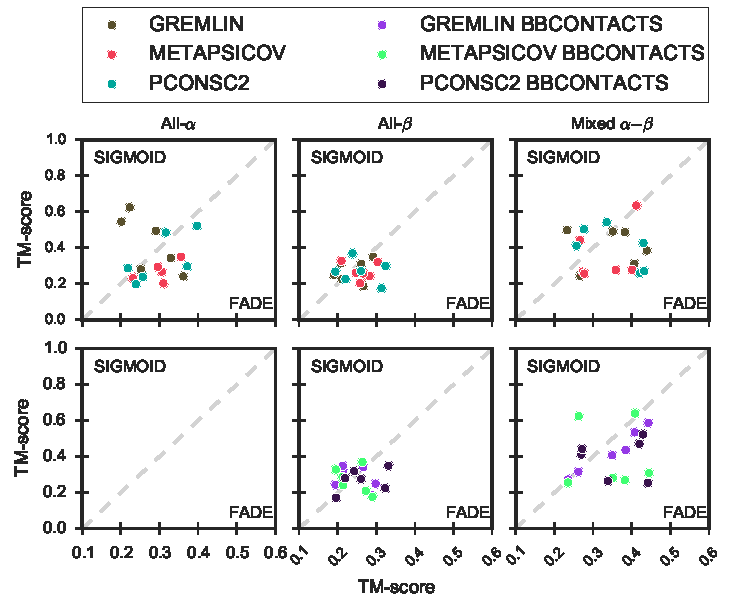
\includegraphics[width=\textwidth]{ample_predictors_tmmedian.pdf}
        \caption{}
        \label{fig:ample_predictor_tmmedian}
    \end{subfigure}

    \begin{subfigure}[b]{0.90\textwidth}
        \centering
        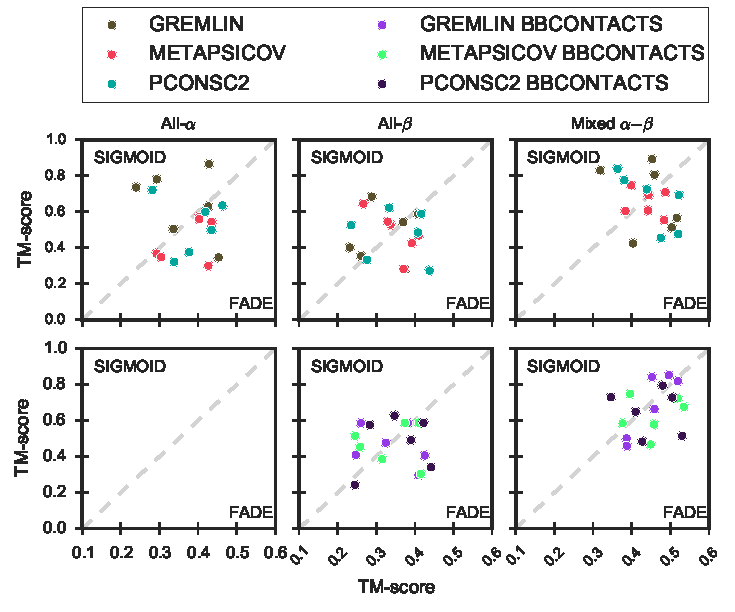
\includegraphics[width=\textwidth]{ample_predictors_tmtop.pdf}
        \caption{}
        \label{fig:ample_predictor_tmtop}
    \end{subfigure}
    \caption[TM-score comparison between ROSETTA energy functions]{(a) Median and (b) top-1 decoy TM-score comparison of FADE and SIGMOID ROSETTA energy functions differentiated by fold and the addition of BBCONTACTS restraints.}
\end{figure}

A \gls{kde} of TM-scores using each predicted decoy was generated with the TM-scores of individual decoys separated only by fold class and ROSETTA energy function (\cref{fig:ample_predictor_tmdensity}). This density estimate further supported the results presented above: the FADE energy function generated more accurate decoys. However, a very important detail was highlighted by the \gls{kde}s. Distinct regions with high density are visible in the estimates of the TM-scores of individual decoys for all-\textalpha\ and mixed \textalpha-\textbeta\ targets (\cref{fig:ample_predictor_tmdensity}). The bimodal distribution of decoy TM-scores from both energy functions strongly suggested that predicted structures were either native-like or not (based on the TM-score threshold of $\leq0.5$). However, the number of correctly predicted decoys versus incorrectly predicted decoys was in favour of the latter. The decoy sets of all-\textbeta\ targets did not show such distinct regions of high density for decoys with TM-scores of less than 0.5 in any of its \gls{kde}s (\cref{fig:ample_predictor_tmdensity}). The generally poor decoy quality of decoys predicted without any predicted distance restraint information (ROSETTA) highlighted the benefit of contact predictions to \textit{ab initio} protein structure prediction.

\begin{figure}[H]
    \centering
    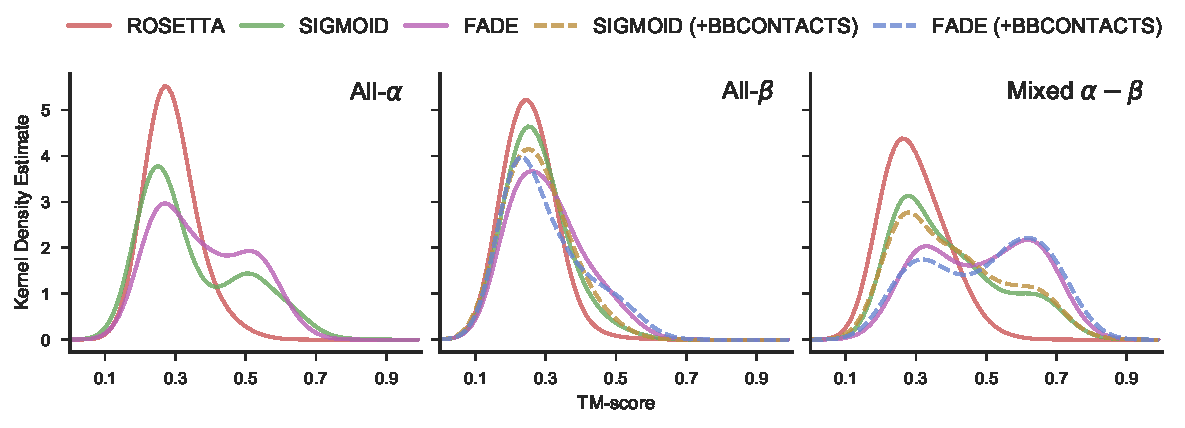
\includegraphics[width=\textwidth]{ample_predictors_tmdensity.pdf}
    \caption[TM-score distribution by fold category and ROSETTA energy function]{\Gls{kde}s of TM-scores of all decoys in each respective fold class separating by ROSETTA energy function (SIGMOID or FADE) and no contact information used (ROSETTA). Dashed lines indicate decoys which were predicted with the addition of BBCONTACTS predictions.}
    \label{fig:ample_predictor_tmdensity}
\end{figure}

A further important aspect of the presented work is the demonstration of the benefits of BBCONTACTS prediction addition to the \textit{ab initio} protein structure prediction of \textbeta-containing targets. Although previous results described in \cref{chap:proof_of_principle} in combination with those presented above outlined overall improvements in decoy quality, it was essential to understand which targets benefit from this treatment. Figure \ref{fig:ample_predictor_bbdir} highlights the effects of adding BBCONTACTS restraints to the structure prediction strategies employed here. In summary, the addition of BBCONTACTS restraints hardly affecte the decoy quality of most targets under the various contact prediction and energy function combinations. Nevertheless, three target, contact prediction and energy function combinations yielded TM-score improvements of at least 0.1 TM-score units compared to the same condition without the addition of BBCONTACTS restraints. In contrast, the addition of BBCONTACTS restraints did not lower the median TM-score by more than 0.1 for any target (\cref{fig:ample_predictor_bbdif}).

\begin{figure}[H]
    \centering
    \begin{subfigure}[b]{\textwidth}
        \centering
        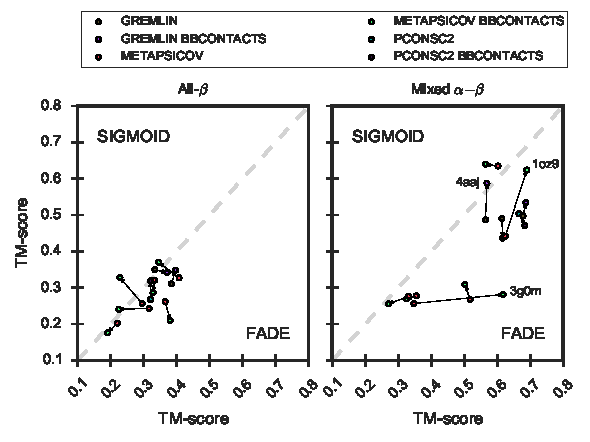
\includegraphics[width=0.9\textwidth]{ample_predictors_bbdir.pdf}
        \caption{}
        \label{fig:ample_predictor_bbdir}
    \end{subfigure}
    
    \begin{subfigure}[b]{\textwidth}
        \centering
        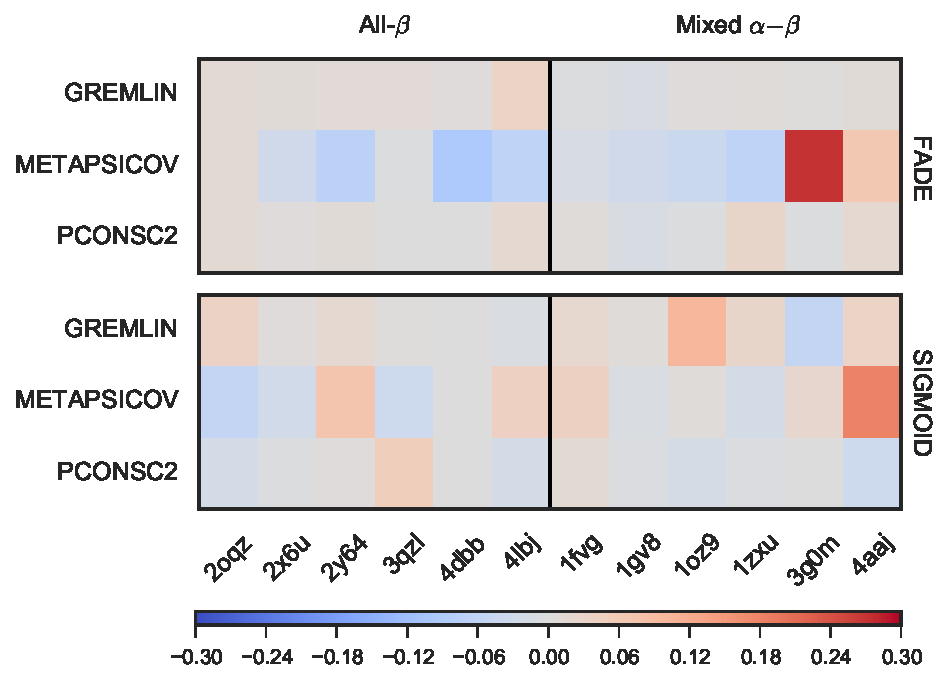
\includegraphics[width=0.8\textwidth]{ample_predictors_bbdif.pdf}
        \caption{}
        \label{fig:ample_predictor_bbdif}
    \end{subfigure}

    \caption[Median TM-score analysis by fold category and ROSETTA energy function]{Median TM-score comparison of FADE and SIGMOID ROSETTA energy functions differentiated by fold (excl. all-\textalpha). (a) Arrows indicate the effect on decoy quality through the addition of BBCONTACTS restraints. Targets with a distance $<0.03$ TM-score units between normal and BBCONTACTS-added conditions were excluded from the scatter plots. (b) Effect on decoy quality through the addition of BBCONTACTS restraints highlighted by heatmap difference. The color scale corresponds to the difference in median TM-score between normal and BBCONTACTS-added contact maps.}
\end{figure}

Two further aspects in understanding the differences in effects of the FADE and SIGMOID ROSETTA energy functions on decoy quality were the target chain length and restraints precision. The former appeared to affect the final decoy quality of all 1,000 decoys insignificantly (\cref{fig:ample_predictor_tmsummary}). However, the restraint precision resulted in some differences between the two ROSETTA energy functions (\cref{fig:ample_predictor_tmsummary}). The FADE energy function (top-\textit{L} restraints) generally appeared to be less sensitive to restraint lists with higher \gls{fp} contact pairs.  In contrast, the SIGMOID function  (3\textit{L}/2 restraints) produced less accurate decoys than the FADE function with more accurate restraints. Most strikingly, the FADE energy function generated decoys with a median TM-score of 0.678 for the N-(5'-phosphoribosyl)anthranilate isomerase domain (\gls{pdb}: 4aaj) compared to the SIGMOID function with a median TM-score of 0.498. Nevertheless, both energy functions appeared to broadly follow a positive linear trend, i.e. better restraint precision resulted in more accurate decoys.

\begin{figure}[H]
    \centering
    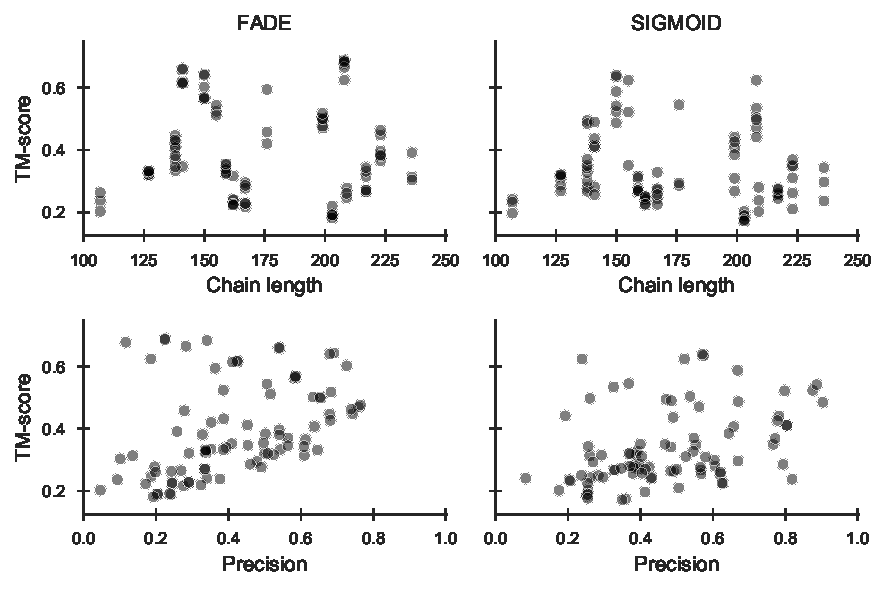
\includegraphics[width=\textwidth]{ample_predictors_tmsummary.pdf}
    \caption[Influence of target chain length and restraint precision on TM-score]{Effects of target chain length and restraint precision on the median TM-score for FADE and SIGMOID ROSETTA energy functions. Each scatter point represents a 1,000-decoy set.}
    \label{fig:ample_predictor_tmsummary}
\end{figure}

\subsection{Impact of metapredictors and energy functions on AMPLE}
The results obtained from the decoy quality comparison outlined in the previous section highlighted differences between the FADE and SIGMOID ROSETTA energy functions. This difference was more pronounced for some targets and did not generalise well in favour of one energy function. Thus, the next step in this study was to analyse the consequences  of these differences for unconventional \gls{mr} using the automated pipeline AMPLE.

Overall, the decoys restrained with GREMLIN distance restraints via the SIGMOID energy function throughout the \textit{ab initio} protein structure prediction process yielded six out of 18 possible structure solutions (\cref{fig:ample_predictor_ample}). This result was the highest of all trialled conditions and only resulted in one more structure solution compared to unrestrained ROSETTA decoys. All remaining conditions resulted in fewer structure solutions than those from ROSETTA decoys. Furthermore, the conditions METAPSICOV (FADE function), METAPSICOV BBCONTACTS (FADE function) and PCONSC2 BBCONTACTS (FADE function) yielded no more than half of the structure solutions achieved by GREMLIN (SIGMOID function). The remaining two conditions --- PCONSC2 (FADE function) and GREMLIN+BBCONTACTS (FADE function) --- resulted in four out of 18 structure solutions. The addition of BBCONTACTS did not improve decoy quality enough to increase the chances of structure solution success; however, the structure of the bovine peptide methionine sulfoxide reductase (\gls{pdb}: 1fvg) was only solved with the GREMLIN+BBCONTACTS (FADE function) decoys further supporting the small but important value of BBCONTACTS restraint addition to separately determined contact predictions.

\begin{figure}[H]
    \centering
    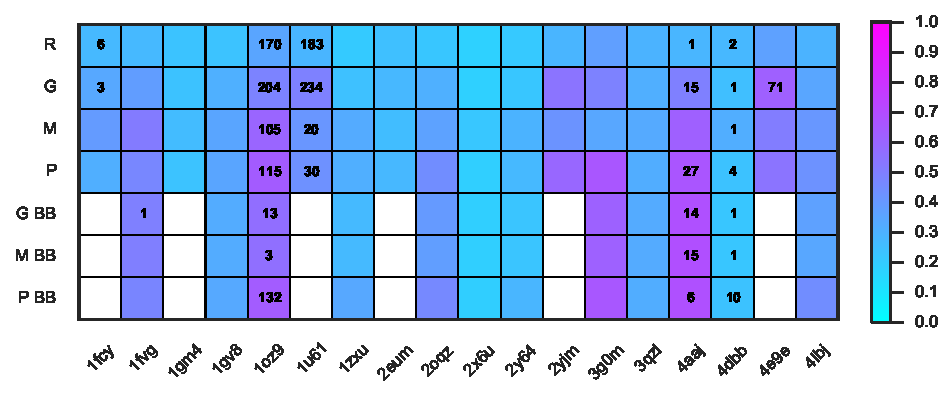
\includegraphics[width=\textwidth]{ample_predictors_ample.pdf}
    \caption[Structure solution count forom AMPLE-derived search models]{Structure solution count for AMPLE search models generated from decoys with varying contact prediction and ROSETTA energy function conditions: unrestrained ROSETTA (R); GREMLIN (G; SIGMOID function); METAPSICOV (M; FADE function); PCONSC2  (P; FADE function); GREMLIN+BBCONTACTS (G BB; FADE function); METAPSICOV+BBCONTACTS (M BB; FADE function); PCONSC2+BBCONTACTS (P BB; FADE function). The colour scale of each square indicates the median TM-score of all 1,000 starting decoys.}
    \label{fig:ample_predictor_ample}
\end{figure}

The number of structure solutions obtained from the decoy sets subjected to the AMPLE pipeline were somewhat surprising given that ROSETTA decoys resulted in the second-most structure solutions. These results suggested that AMPLE was unable to exploit the true value of more accurate decoy sets. This hypothesis was further supported when considering the decoy set quality and the number of structure solutions (\cref{fig:ample_predictor_ample}). For example, PCONSC2 (FADE function) decoys predicted for the hypothetical protein AQ\_1354 (\gls{pdb}: 1oz9) showed high accuracy, and thus would generally be considered highly desirable starting structures for the AMPLE protocol. Nevertheless, the AMPLE protocol was unable to exploit these decoys for successful \gls{mr} structure solution. Similarly, the high-accuracy contact-assisted decoys sets predicted for other targets, e.g. cysteine desulferation protein SufE (\gls{pdb}: 3g0m; median TM-score PCONSC2+BBCONTACTS (FADE function)=0.661) also failed to result in \gls{mr} solutions. In comparison, the median TM-scores for all successful ROSETTA decoy sets did not exceed 0.355 TM-score units, which suggested that the AMPLE routine may be optimised for less accurate ROSETTA decoys.

Naturally, one would expect the best decoys to result in the most accurate ensemble search models, which in turn yield the highest number of structure solutions per target. However, here we demonstrated that the most accurate decoys did not guarantee structure solution, and in contrast some poorly predicted decoy sets achieved structure solution. Thus, it was essential to investigate the stage in AMPLE's cluster-and-truncate approach at which the higher decoy quality resulted in less suitable ensemble search models for \gls{mr}.

\begin{figure}[H]
    \centering
    \begin{subfigure}[b]{0.49\textwidth}
        \centering
        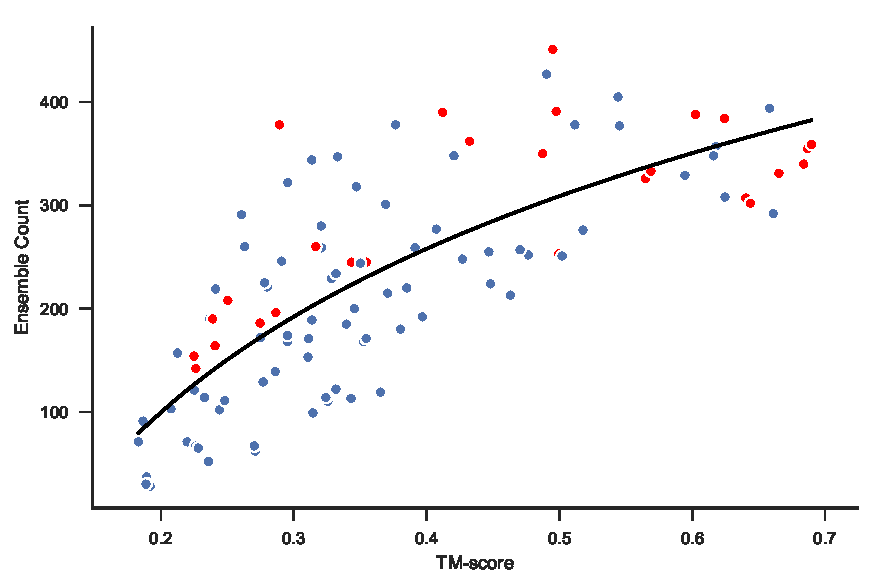
\includegraphics[width=\textwidth]{ample_predictors_ensdep.pdf}
        \caption{}
        \label{fig:ample_predictor_ensdep}
    \end{subfigure}
    %
    \begin{subfigure}[b]{0.49\textwidth}
        \centering
        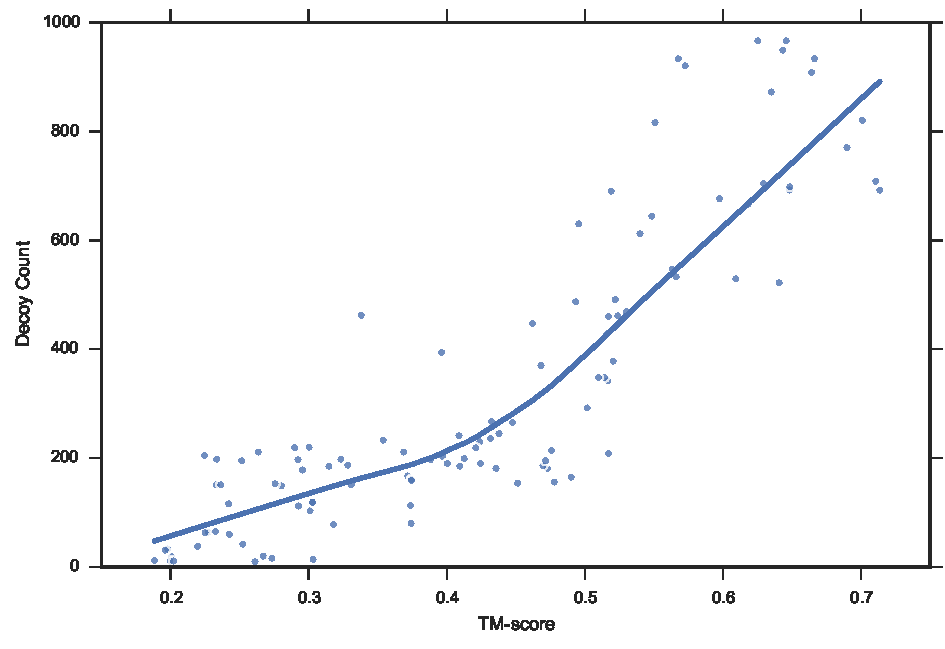
\includegraphics[width=\textwidth]{ample_predictors_clusizetm.pdf}
        \caption{}
        \label{fig:ample_predictor_clusizetm}
    \end{subfigure}

    \caption[Relationship between TM-score, AMPLE search model size and SPICKER cluster count]{(a) Comparison of median TM-score (per 1,000 decoys) against the resulting AMPLE ensemble search model count. The equation of the line of best fit is defined by $y=228.50*\ln\left(20.96*x\right)-227.95$. Red dots indicate successful ensemble sets. (b) Relationship between cluster median TM-score and the number of cluster decoys. Blue line represents line of best fit with equation $y=148.85*\exp\left(2.90*x\right)-225.76$.}
\end{figure}

The data generated as part of this study reveale a positive correlation ($\rho_{Spearman}=0.78$; $p<0.001$) between the decoy quality and the number of resulting AMPLE ensemble search models. In \cref{fig:ample_predictor_ensdep}, the plotted data alongside a line of best fit further illustrate that small differences in decoy quality in the lower TM-score regions increased the total number of generated ensemble search models dramatically. However, once the threshold of 0.5 TM-score units was surpassed the number of generated ensemble search models plateaued at around ~350-400 ensemble search models, approaching the maximum number of search models generatable by AMPLE. Furthermore, the data suggested that sets containing fewer than 100 ensemble search models did not lead to structure solution, although this result needed to be considered with care given the difficulty of predicting which search model will lead to structure solution.

\begin{figure}[H]
    \begin{subfigure}[b]{\textwidth}
        \centering
        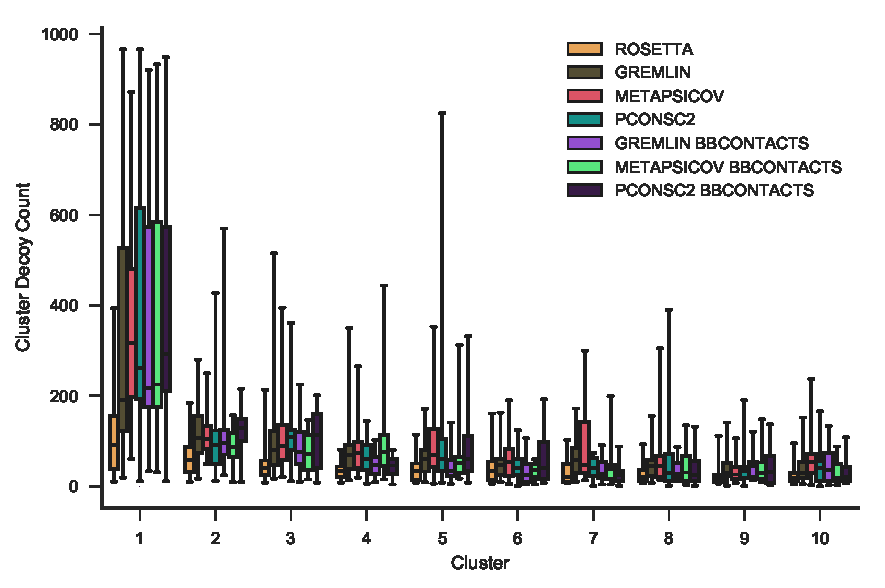
\includegraphics[width=0.9\textwidth]{ample_predictors_clusize.pdf}
        \caption{}
        \label{fig:ample_predictor_clusize}
    \end{subfigure}

    \begin{subfigure}[b]{\textwidth}
        \centering
        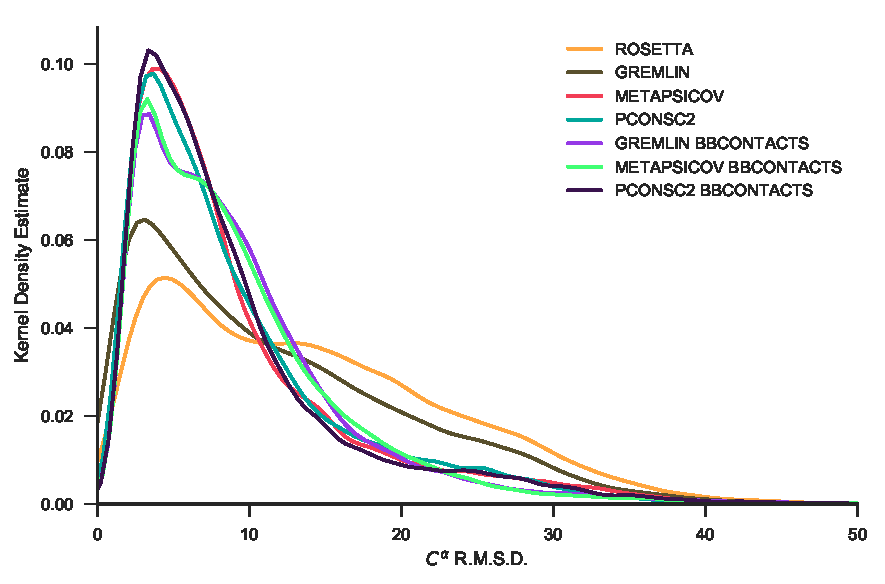
\includegraphics[width=0.9\textwidth]{ample_predictors_carmsd.pdf}
        \caption{}
        \label{fig:ample_predictor_carmsd}
    \end{subfigure}
    \caption[Effects of decoy sets on SPICKER clustering]{(a) SPICKER cluster sizes of each target grouped the restraint condition used during the structure prediction protocol. Whiskers span the range from the minimum to maximum counts. (b) \Gls{kde} of C\textalpha\ interatomic \gls{rmsd} for SPICKER clusters.}
\end{figure}

Besides looking at the relationship between entire decoy sets and the resulting structure solutions on a per-target or per-condition basis, it was important to also consider individual ensemble search models, their origins and their properties in relation to \gls{mr} metrics. Findings outlined in \cref{chap:proof_of_principle} highlighted the relationship between the number of decoys in the first cluster and its decoy quality (see \cref{chap:proof_of_principle}). Here, further support for these findings was given by means of the positive relationship between the median TM-scores and the corresponding size of the largest SPICKER cluster (\cref{fig:ample_predictor_clusizetm}). An analysis of the cluster sizes demonstrated the downstream benefits of increased decoy quality through contact restraints in the folding process (\cref{fig:ample_predictor_clusize}). The sizes of the first three clusters generated from most contact-restraint decoy sets greatly surpassed their equivalent cluster sizes for unrestrained ROSETTA decoys. Given that cluster sizes correlated with decoy quality, these results also supported the idea that the mean C\textalpha\ \gls{rmsd} --- as calculated by THESEUS for cluster truncation --- was directly related to better decoy quality via the larger number of decoys in each cluster (\cref{fig:ample_predictor_clurmsd}). The same mean C\textalpha\ \gls{rmsd} was also related to the number of ensemble search models generated after subclustering (\cref{fig:ample_predictor_rmsdsm}), which hinted towards a direct relationship between increased quality of 1,000 decoys per set and the total number of ensemble search models generated. Interestingly, GREMLIN decoys showed similar C\textalpha\ \gls{rmsd} per cluster compared to unrestrained ROSETTA decoys (\cref{fig:ample_predictor_carmsd}), unlike all other contact-restraint-guided structure predictions. However, it is worth noting that almost no distinction could be made amongst the remaining contact restraint treatments despite some differences in cluster size distributions exist (\cref{fig:ample_predictor_clusize}).

\begin{figure}[H]
    \centering
    \begin{subfigure}[b]{0.49\textwidth}
        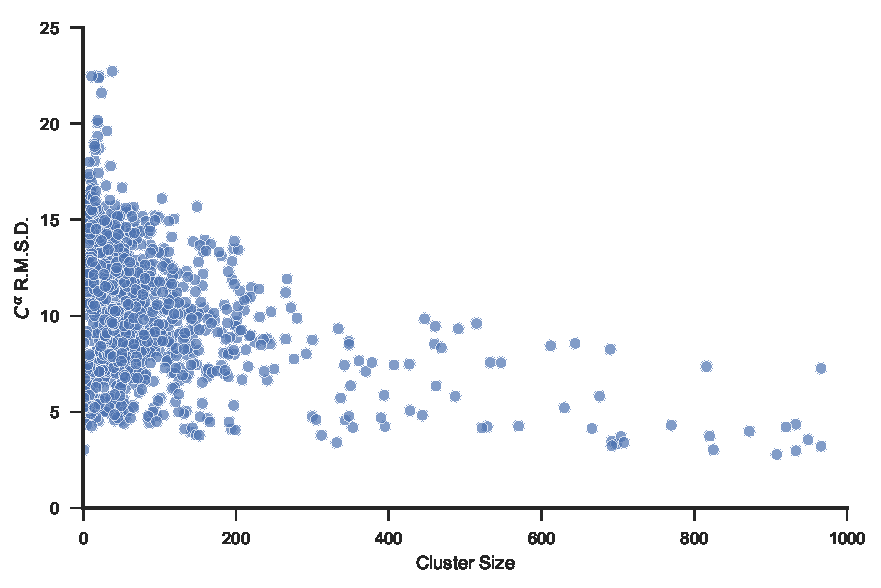
\includegraphics[width=\textwidth]{ample_predictors_clurmsd.pdf}
        \caption{}
        \label{fig:ample_predictor_clurmsd}
    \end{subfigure}
    % 
    \begin{subfigure}[b]{0.49\textwidth}
        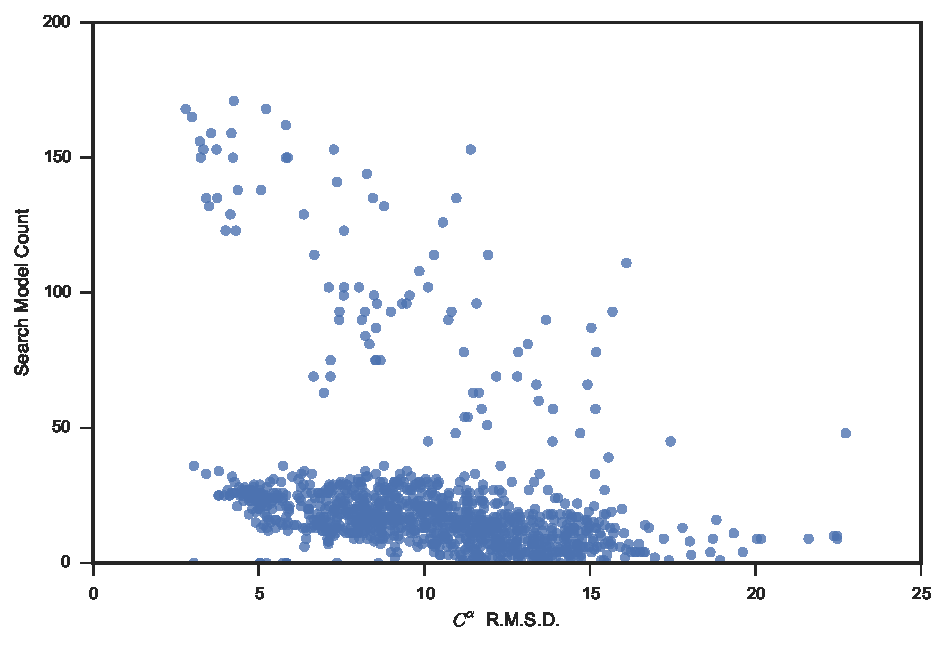
\includegraphics[width=\textwidth]{ample_predictors_rmsdsm.pdf}
        \caption{}
        \label{fig:ample_predictor_rmsdsm}
    \end{subfigure}

    \caption[SPICKER cluster properties]{(a) Number of decoys per SPICKER cluster plotted against the mean C\textalpha-atom \gls{rmsd} for all decoys in each cluster. (b) Mean C\textalpha-atom \gls{rmsd} for decoys per cluster plotted against the number of search models derived from the cluster.}
\end{figure}

The structure solution through pipelines like AMPLE and other unconventional \gls{mr} software \cite{Rodriguez2012-ad,Sammito2013-ug} can result from the placement of generated (ensemble) search models either in- or out-of-sequence register. The RIO metric \cite{Thomas2015-wu} can reliably assess the register placement, and thus was used to analyse the \gls{mr} placements of all search models of the seven targets with structure solutions from one or more decoy sets. The RIO scores for the hypothetical protein AQ\_1354 (\gls{pdb}: 1oz9) strongly supported the high quality decoys used as input across all seven contact conditions (\cref{fig:ample_predictor_riotar}). Most search models were placed in-register and hardly any search models with out-of-register RIO scores failed either. In contrast, the search models of N-(5’-phosphoribosyl)anthranilate isomerase (\gls{pdb}: 4aaj) --- derived from high quality decoys in most conditions --- showed a low percentage of AMPLE search models with RIO scores leading to structure solution (\cref{fig:ample_predictor_riotar}). Furthermore, the RIO scores normalized by the target chain length indicated that search models, independent of \gls{mr} structure solution, were relatively small only exceeding 20\% of the total target sequence in a few cases. 

\begin{figure}[H]
    \centering
    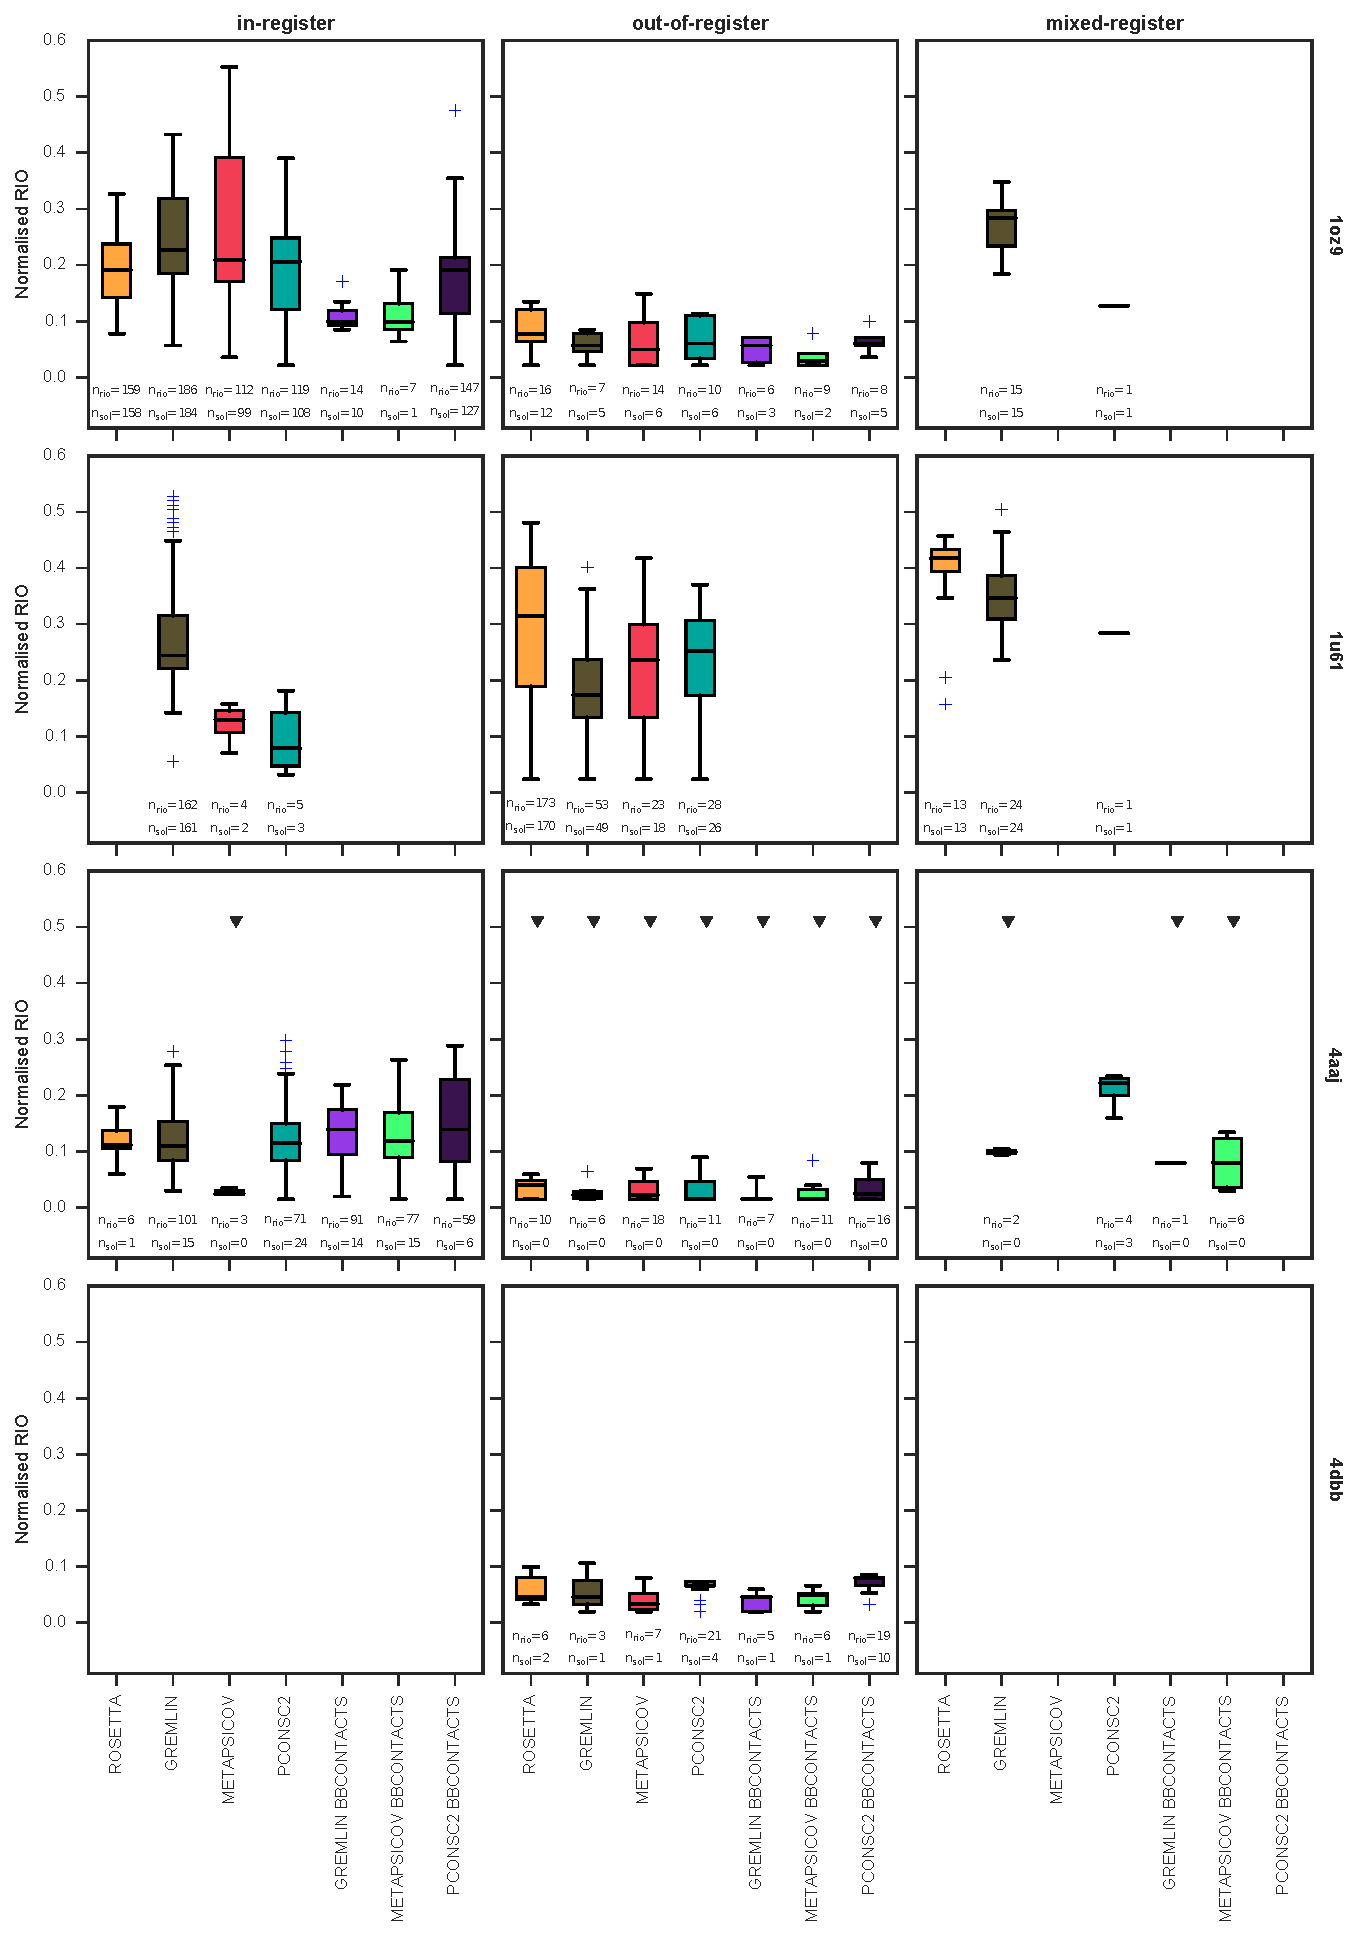
\includegraphics[width=0.95\textwidth]{ample_predictors_riotar.pdf}
    \caption[RIO score analysis of successful targets]{Normalised RIO score analysis of four successful targets in the \gls{mr} dataset. Black triangles indicate AMPLE search model sets without a structure solution.}
    \label{fig:ample_predictor_riotar}
\end{figure}

One interesting target in this set with respect to the sequence register of the AMPLE search models leading to structure solution was the putative ribonuclease III (\gls{pdb}: 1u61) domain. Although decoys from all contact conditions readily solved this target with at least 20 or more AMPLE search models, one important aspect arose from the RIO register analysis. Only GREMLIN decoys were primarily placed in-register (\cref{fig:ample_predictor_riotar}). AMPLE search models derived from the other three contact conditions, and in particular those from ROSETTA decoys, wereprimarily placed out-of-register with sequence coverage values of roughly 25\%. A close analysis of the diversity of AMPLE search models highlighted the accuracy of GREMLIN search models which represented a closely-matched substructure of the target protein (\cref{fig:ample_predictors_1u61_c2_t70_r1_reliable}).  

\begin{figure}[H]
    \begin{subfigure}[b]{0.49\textwidth}
        \centering
        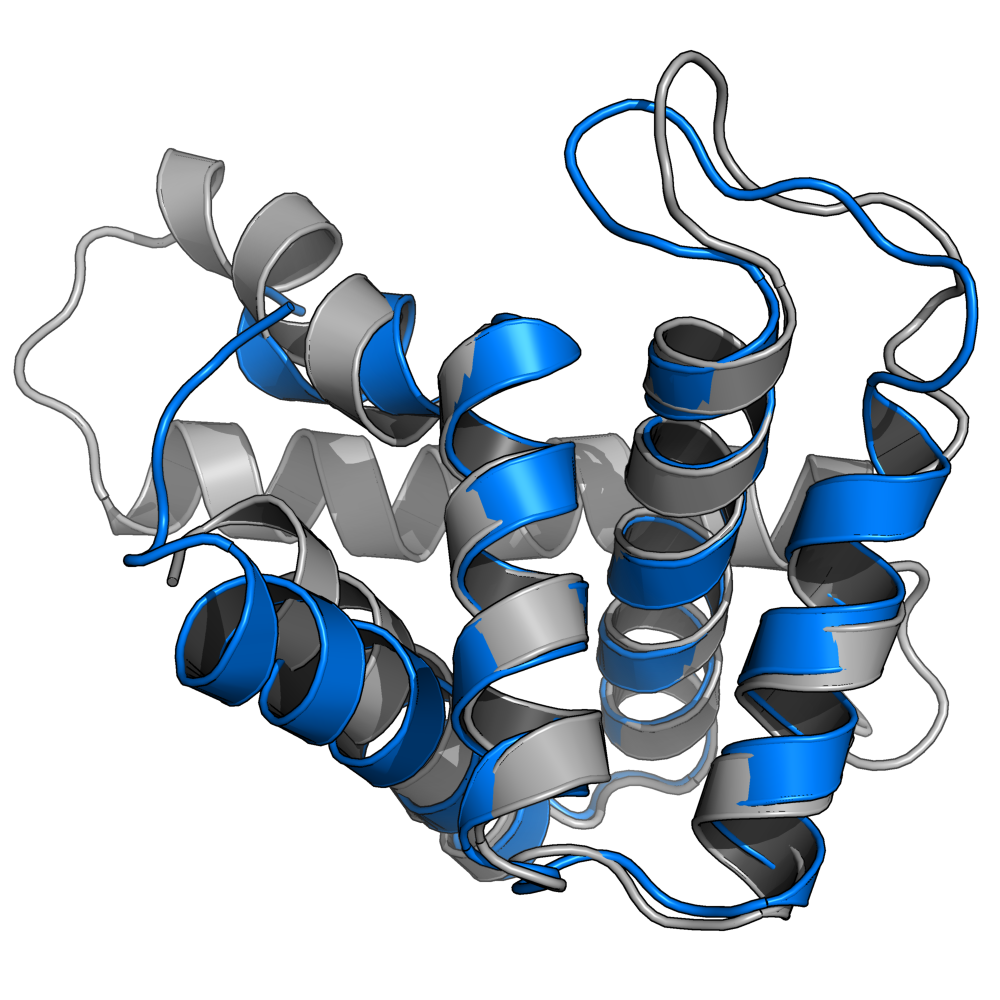
\includegraphics[width=0.8\textwidth]{ample_predictors_1u61_c2_t70_r1_reliable.png}
        \caption{}
        \label{fig:ample_predictors_1u61_c2_t70_r1_reliable}
    \end{subfigure}
    %
    \begin{subfigure}[b]{0.49\textwidth}
        \centering
        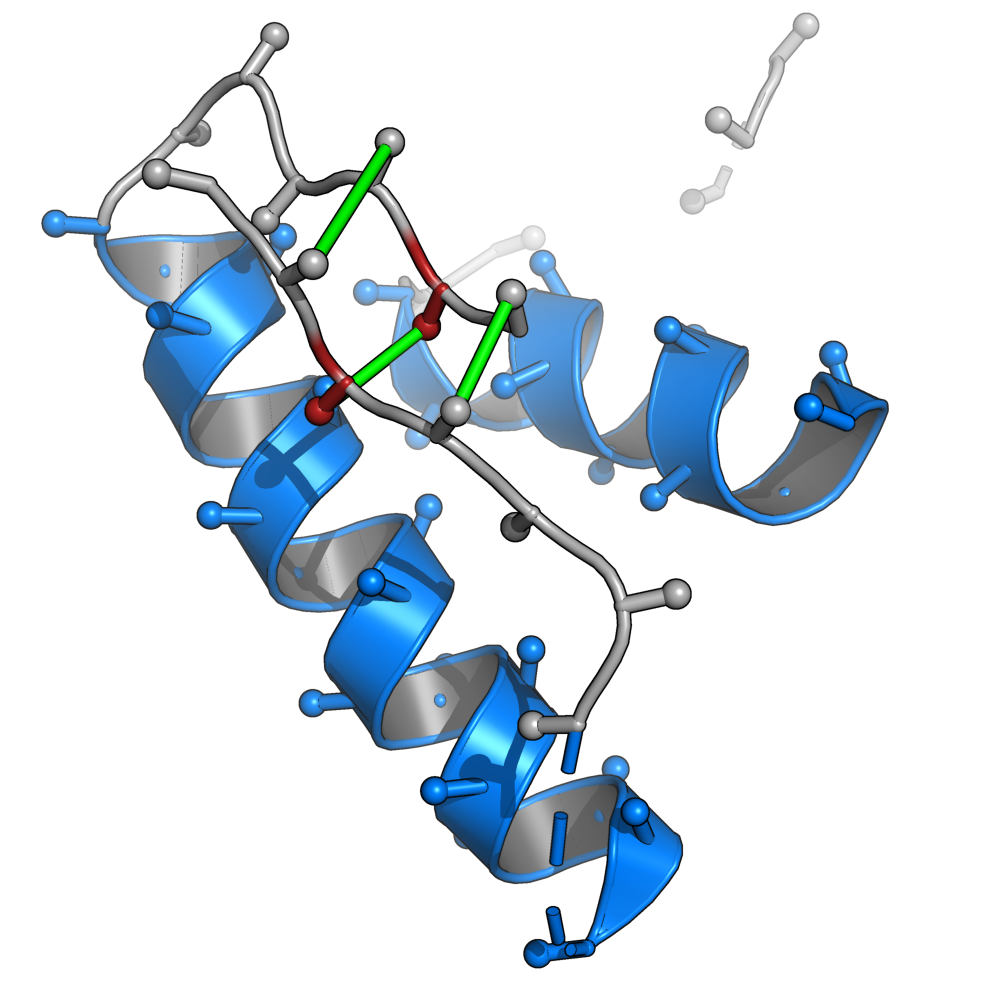
\includegraphics[width=0.8\textwidth]{ample_predictors_1fvg_gbb_phaser_c1_t25_r3_polyAla.png}
        \caption{}
        \label{fig:ample_predictors_1fvg_gbb_phaser_c1_t25_r3_polyAla}
    \end{subfigure}
    \caption[Examples of successfully placed AMPLE search models]{AMPLE ensemble search models post-PHASER placement for (a) putative ribonuclease III (\gls{pdb}: 1u61) and (b) peptide methionine sulfoxide reductase (\gls{pdb}: 1fvg). Search models (blue) are superposed to their native crystal structures (grey). BBCONTACTS distance restraints are represented as green lines. Secondary structure assignment calculated with STRIDE \cite{Frishman1995-si}. In (b), red residues indicate \textbeta-strand residues.}
\end{figure}

Compared to all other targets with structure solutions in at least one condition, the PTB domain of Mint1 (\gls{pdb}: 4dbb) produced similarly interesting yet somewhat surprising results. None of the search models, independent of their decoy source, had any residues placed in-register. All structure solutions were obtained from out-of-register search model placements (\cref{fig:ample_predictor_riotar}). A visual inspection of all successful search models revealed that structure solutions were exclusively obtained with idealised fragments. ROSETTA, GREMLIN and METAPSICOV decoys resulted in one or more single-helix ensemble search models that led to structure solution (\cref{fig:ample_predictors_4dbb_esm_egs}). More interestingly though, PCONSC2, GREMLIN+BBCONTACTS, METAPSICOV+BBCONTACTS and PCONSC2+BBCONTACTS decoys yielded one or more two-strand \textbeta-sheets which, after successful \gls{mr}, yielded fully built structures (\cref{fig:ample_predictors_4dbb_esm_egs}).

\begin{figure}[H]
    \centering
    \includegraphics[width=\textwidth]{ample_predictors_4dbb_esm_egs.png}
    \caption[Example of successfully placed AMPLE search model]{Successful search models post-PHASER placement (blue) superposed to the reference crystal structure (grey) for PTB domain of Mint1 (\gls{pdb}: 4dbb).}
    \label{fig:ample_predictors_4dbb_esm_egs}
\end{figure}

Lastly, three targets were solved with one or two decoy sets alone. The structures of the retinoic acid nuclear receptor HRAR (\gls{pdb}: 1fcy) and the peptide methionine sulfoxide reductase (\gls{pdb}: 1fvg) were only solved with a handful of AMPLE search models. Often singleton solutions like these are achieved through AMPLE's cluster-and-truncate procedure producing a single, idealised helix as search model. Here, the data confirmed this for target 1fcy, whereby single out-of-register helices derived from ROSETTA and GREMLIN decoys achieved structure solutions. However, the singleton search model derived from the GREMLIN+BBCONTACTS decoys for the peptide methionine sulfoxide reductase (\gls{pdb}: 1fvg) was placed in-register. A closer inspection of this AMPLE ensemble search model highlighted a great success of the approach of adding BBCONTACTS distance restraints to separately predicted base contact maps. In this instance, the successful AMPLE ensemble search model had 77\% of its 49 residues placed in-register. More importantly, the search model was made up of two \textbeta-strands packing against each other, which was supported by BBCONTACTS predictions (\cref{fig:ample_predictors_1fvg_gbb_phaser_c1_t25_r3_polyAla}). The last case, glycosylase domain of MBD4 (\gls{pdb}: 4e9e), solved solely with GREMLIN decoys yielding 71 structure solutions. All successful AMPLE search models derived from the GREMLIN decoys were placed in-register.

\section{Discussion}
This study was designed to explore the state-of-the-art metapredictor pipelines for residue-residue contact prediction. The main focus of this work was to distinguish differences in three key parts: raw contact predictions, their use in  \textit{ab initio} structure prediction and finally the effects on unconventional \gls{mr} using AMPLE.

Key findings in this study revealed METAPSICOV and PCONSC2 metapredictors to yield the most precise contact predictions regardless of target fold or size. These results are in line with previous findings, which independently confirmed METAPSICOV contact predictions to yield the highest precision across numerous prediction algorithms \cite{Wuyun2016-hh, De_Oliveira2017-gj}. However, work in this study cannot confirm their findings, which demonstrated more precise contact predictions for all-\textbeta\ and mixed \textalpha-\textbeta\ protein targets compared to all-\textalpha\ ones. Several reasons might give insights into this discrepancy: (1) a much smaller sample size was trialled in this study (\textcite{Wuyun2016-hh}: 680; \textcite{De_Oliveira2017-gj}: ~3500); (2) the targets were chosen to deliberately sample various alignment depths including relatively low alignment depth ($<200$) values; (3) only final contact predictions were analysed, thus benefiting from post-prediction consensus finding and contact map processing through unsupervised machine-learning algorithms.

Furthermore, the results obtained in this study demonstrated that two similar ROSETTA energy functions yield different structure prediction results. The FADE function on average achieves more accurate structure predictions compared to the SIGMOID one. This result seems striking at first; however, a closer inspection of each of the energy function parameters gives possible insights into the reasons for the different outcomes. The FADE energy function defines both a maximum and minimum distance. The FADE energy function also does not consider amino acid-specific distances while the SIGMOID function does \cite{Kamisetty2013-le}. Furthermore, a custom weight factor is added for SIGMOID restraints to balance the restraint term in the overall energy term of each decoy (Sergey Ovchinnikov, personal communication). Thus, small changes in each of those definitions could have significant effects on the final structure prediction. Unfortunately, it is out of the scope of this study to explore all variations, and thus results aid primarily as guide for future work and AMPLE users. This study highlighted again the benefits of adding BBCONTACTS predictions to existing contact maps to further restrain \textbeta-rich regions during \textit{ab initio} protein structure prediction. 

Lastly, part of the comparison carried out in this study was aimed specifically at \gls{mx} experimentalists and, in particular, AMPLE users. Beyond the proof-of-principle study described in \cref{chap:proof_of_principle}, this work further illustrated how important additional restraint information is to increase the chances of unconventional \gls{mr} success. However, this work also highlighted limitations in the AMPLE routine whereby decoys that were restrained by predicted residue-residue contacts achieved much higher decoy quality compared to unrestrained ROSETTA decoys, yet solved fewer targets. The idea that restrained decoys might benefit from a different kind of processing was further supported by the most successful decoy sets, which were obtained with GREMLIN contact predictions. Given that GREMLIN and ROSETTA decoys achieved similar decoy qualities across multiple targets, their structure solutions were identical for all of ROSETTA's successful solutions. GREMLIN decoys outperformed ROSETTA decoys solely on the basis that it acquired highly accurate decoys for one further target, and thus achieved the most structure solutions in this study. 

Therefore, further work was required to identify the optimal strategy for decoy sets with high structural similarities to the native fold. Such work could focus on the recent idea of selecting decoys based on their long-range contact precision \cite{De_Oliveira2017-gj, Ovchinnikov2017-nd} to specifically eliminate the worst decoys, and thus enhance a more fine-grained clustering approach in SPICKER (\cref{chap:ample_decoys}). Alternatively, truncation could be guided by alternative means, such as the importance of each residue in the predicted contact map. Ultimately, it is key to improve the AMPLE protocol to exploit the much higher decoy quality to enhance the user’s chance of success.


\chapter{Alternative \textit{ab initio} structure prediction algorithms for AMPLE} \label{chap:alternate_abinitio_protocols}
\clearpage
% \chapter{Alternative \textit{ab initio} structure prediction algorithms for AMPLE} \label{chap:alternate_abinitio_protocols}
\clearpage

\textbf{Acknowledgement: }\textit{I would like to thank Dr Saulo de Oliveira for his contributions to this chapter. He kindly provided his time and expertise to generating SAINT2 structure predictions included in the analysis presented in this chapter.}

\section{Introduction}
To-date, the recommended \textit{ab initio} protein structure prediction protocol for optimal AMPLE performance is ROSETTA \cite{Keegan2015-zb,Thomas2017-sh,Thomas2015-wu,Bibby2012-lm}. This recommendation is based primarily on the superiority of the decoy quality compared to other modelling algorithms, which was recently reaffirmed by the CASP12 experiments \cite{Abriata2018-lu,Ovchinnikov2018-wp}. However, \textcite{Keegan2015-zb} demonstrated that the alternative \textit{ab initio} structure prediction protocol QUARK provides a suitable alternative to ROSETTA in AMPLE. Although inferior in the total number of structure solutions, QUARK decoys are a suitable ROSETTA alternative in most cases \cite{Keegan2015-zb}. In particular, given ROSETTA's challenging installation procedure, availability limited to POSIX operating systems, requirement for large disk space and computationally expensive algorithm, QUARK's online server has been a very attractive alternative for AMPLE users.

Whilst ROSETTA and QUARK are amongst the best \textit{ab initio} structure prediction algorithms currently available \cite{Abriata2018-lu}, other algorithms have been developed over the last two decades \cite[e.g.,][]{Jones2001-mc,Ellis2010-zs,Adhikari2015-lb,Xu2012-jf,Marks2011-os,Wang2016-ar}. Although most of these algorithms utilise fragment-assembly algorithms similar to ROSETTA and QUARK, their procedures for fragment selection or assembly is substantially different \cite{Ellis2010-zs,Jones2001-mc}. Furthermore, predicted contact information has recently seen a spike in precision. This invaluable source of information is introduced differently in each protocol, and thus might have profound effects on the resulting decoy quality. In particular, physics-based algorithms relying largely on this information are an interesting alternative to fragment-based approaches \cite{Adhikari2015-lb,Marks2011-os,Wang2016-ar,Dos_Santos2018-lq}.

CONFOLD2 \cite{Adhikari2018-lj}, a distance-geometry based algorithm, uses predicted secondary structure and contact information to rapidly generate \textit{ab initio} decoys. Unlike other algorithms, CONFOLD2's algorithm is driven almost entirely by the contact information to explore the fold space. Different contact selection thresholds are used to not limit the search space to a fixed, predefined selection. CONFOLD2 generates slightly less accurate decoys compared to ROSETTA, however outperforms it in speed and simplicity of installation \cite{Adhikari2018-lj,Michel2017-xh}.

FRAGFOLD \cite{Jones2001-mc}, a fragment-assembly based algorithm, generates decoys in a similar fashion to ROSETTA and QUARK. However, FRAGFOLD does not rely on large structural libraries for fragment extraction. Instead, it provides a relatively small library of supersecondary structural fragments and short length fragments, which were extracted from high resolution protein structures. Since the generalised fragment library is shipped with FRAGFOLD, and target-specific fragments are extracted based on secondary structure and a sequence-based threading score, fragment library generation is fast and easy compared to ROSETTA \cite{Kosciolek2014-bt}.

SAINT2 \cite{De_Oliveira2018-sg}, a further fragment-assembly based algorithm is substantially different to most others. SAINT2 attempts \textit{ab initio} structure prediction sequentially, starting from either terminus of the target sequence \cite{De_Oliveira2018-sg}. Furthermore, SAINT2 uses FLIB \cite{De_Oliveira2015-kb} for fragment picking, an algorithm shown to outperform ROSETTA's equivalent NNMAKE \cite{Gront2011-sv} in precision with very similar coverage.

Since some of these algorithms are readily available and often easier to install without the overhead of large databases for fragment picking, the work in this study focused on exploring three alternative \textit{ab initio} structure prediction algorithms and their value in unconventional \gls{mr}. The \textit{ab initio} structure prediction protocols CONFOLD2 \cite{Adhikari2018-lj}, FRAGFOLD \cite{Jones2001-mc} and SAINT2 \cite{De_Oliveira2018-sg}, were benchmarked in AMPLE given their substantially different approaches to AMPLE's current default ROSETTA \cite{Rohl2004-dj}.

\section{Materials \& Methods}
\subsection{Target selection}
This study was conducted using all 27 targets from the PREDICTORS dataset (\cref{sec:methods_dataset_predictors} and \cref{table:appendix_dataset_predictors}).

\subsection{Contact prediction}
Residue-residue contact information was predicted for 18 out of 27 targets using METAPSICOV v1.04 \cite{Jones2015-vq}. Nine targets were left deliberately without contact prediction to trial the performance of each algorithm under such circumstances.

Secondary structure and solvent exposure were predicted using PSIPRED v4.0 \cite{Jones1999-ed} and SOLVPRED (shipped with METAPSICOV v1.04), respectively. The \gls{msa} for coevolution-based contact prediction was generated using HHBLITS v2.0.16 \cite{Remmert2011-kt} against the \texttt{uniprot20} v2016-02 database. CCMPRED v0.3.2 \cite{Seemayer2014-zp}, FREECONTACT v1.0.21 \cite{Kajan2014-bx} and PSICOV v2.1b3 \cite{Jones2012-ks} were used by METAPSICOV to generate contact predictions.

METAPSICOV STAGE1 contact predictions were used in \textit{ab initio} structure prediction since they result in more accurate \textit{ab initio} protein structure predictions compared to METAPSICOV STAGE2 predictions \cite{Jones2015-vq}.

\subsection{\textit{Ab initio} structure prediction} \label{sec:ample_saint2_modelling}
The ROSETTA 3- and 9-residue fragment libraries for each target were generated using the ROBETTA online server (\url{http://robetta.bakerlab.org/}). The option to ``Exclude Homologues'' was selected to avoid inclusion of homologous fragments. Each target sequence and its fragments were subjected to ROSETTA v2015.22.57859 \cite{Rohl2004-dj} and 1,000 decoys per target generated with AMPLE v1.2.0 ROSETTA default options. Top-$L$ (where $L$ corresponds to the number of residues in the target chain) contact pairs were used in combination with the \textit{FADE} ROSETTA energy function. For further details see \cref{sec:ample_proof_con2res} or \textcite{Michel2014-eg}.

The FRAGFOLD decoys were generated using FRAGFOLD v4.80 \cite{Jones2001-mc} with default options. Homologous fragments were removed from the shipped library  by excluding all entries with \gls{pdb} identifiers identical to those retrieved from the ROBETTA server. All contact pairs were used according to FRAGFOLD's internal protocol.

The fragment libraries for SAINT2 were generated using FLIB \cite{De_Oliveira2015-kb}, which picks on average ~30 fragments per target position. These fragments are typically six to 20 residues in length. Homologous fragments were removed from the final fragment list using the \gls{pdb} identifiers obtained from the ROBETTA online server. The secondary structure prediction and solvent accessibility scores were identical to those obtained from the ROBETTA server. SAINT2 was used for decoy generation, and 1,000 decoys generated per target. The procedure and parameters were identical to those described in Supplementary Information (p. 16) by \textcite{De_Oliveira2018-sg}.

The CONFOLD2 decoys were generated using CONFOLD2 v2.0 \cite{Adhikari2018-lj}, which uses \gls{cns} v1.3 \cite{Brunger1998-sz} to drive the modelling. Default parameters were used except for the number of decoys per run, which was increased from 20 to 25 using the \texttt{-mcount} parameter. CONFOLD2 varies the number of contacts included in each separate modelling run, ranging from $L/10$ to $4L$ with increments of $L/10$. Thus, the CONFOLD2 protocol yields a total of 40 separate modelling runs generating 25 decoys each. Structure predictions for only 18 targets were done since nine targets were benchmarked without any contact predictions, which are an essential input in CONFOLD2.

\subsection{Molecular Replacement}
All decoy sets were subjected to AMPLE v1.2.0 and CCP4 v7.0.28. Default options were chosen with the following exceptions: decoys in all 10 clusters were used, subcluster radii thresholds were set to 1 and 3\AA, and side-chain treatments were set to \texttt{polyala} only. This change in protocol from AMPLE's initial mode of operation \cite{Bibby2012-lm} was shown to be advantageous in most cases by \textcite{Thomas2017-qu}, and thus trialled in this context.  Each \gls{mr} run was assessed using the SHELXE criteria, where a minimum \gls{cc} of 25.0 and \gls{acl} of 10 was required (\cref{sec:methods_mr_success}). R-values of less than 0.45 after model building were not part of the success criteria in this study.

\section{Results}
The purpose of this study was to investigate the usefulness of alternative \textit{ab initio} structure prediction algorithms in AMPLE. Three promising leads widely used in the \textit{ab initio} modelling experiments were examined and compared against AMPLE's current algorithm of choice. This led to a direct comparison of the algorithms ROSETTA \cite{Rohl2004-dj}, CONFOLD2 \cite{Adhikari2018-lj}, FRAGFOLD \cite{Jones2001-mc} and SAINT2 \cite{De_Oliveira2018-sg}. All four algorithms have recently seen great improvements through the use of residue-residue contact information, which was predicted for two-thirds of the targets using the METAPSICOV \cite{Jones2015-vq} algorithm.

\subsection{Alignment depth and contact prediction precision}
The first step in this study was the prediction of residue-residue contacts using the metapredictor METAPSICOV for 18 targets in the PREDICTORS dataset \cite{Jones2015-vq}. Since we attempted to test each of the structure prediction boundaries in extreme cases, a variety of targets with different alignment depths were chosen. The alignment depth --- i.e., the number of effective sequences --- of METAPSICOV-generated HHBLITS alignments ranged from 431 to 6,186 across all targets (\cref{fig:ample_saint2_alndepth}). Six targets contained at least 200 and less than 1,000 sufficiently-diverse sequences, whilst the remaining 16 targets contained more than 1,000 effective sequences.

\begin{figure}[H]
    \centering
    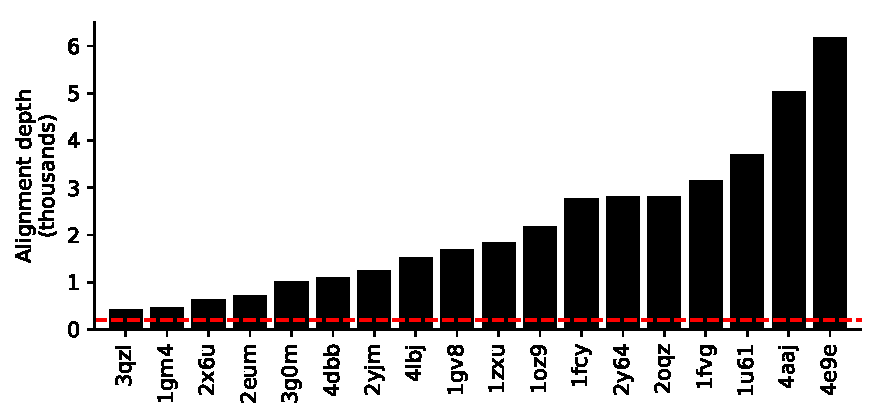
\includegraphics[width=\textwidth]{ample_saint2_alndepth.pdf}
    \caption[Alignment depth for subsets of targets in the PREDICTORS dataset]{Distribution of HHBLITS alignment depth for subset of targets in the PREDICTORS dataset. Red line indicates the suggested alignment depth requirement for accurate coevolution-based contact prediction \cite{Simkovic2017-xs}.}
    \label{fig:ample_saint2_alndepth}
\end{figure}

Coevolution-based contact predictors rely heavily on the alignment depth for accurate contact predictions. In this work, these findings were further confirmed. Sequence alignments with depths of less than 1,000 sequences produced contact predictions with lower precision scores across a number of cutoffs compared to those with deeper alignments (\cref{fig:ample_saint2_conprec}). Given the alignment depths and top-$L$ contact predictions, a positive correlation between the two was found (Spearman's $\rho=0.57$, p-value $<0.02$). A moving average analysis showed that those contact predictions based on alignments with more than 1,000 effective sequences yielded better precision scores by at least 0.09 units up to 0.34. The difference between the two moving average curves in \cref{fig:ample_saint2_conprec} highlights that the difference was greater at lower cutoff values, i.e. only the very best contacts were included in the selection. This difference declined more drastically for targets with deeper alignments (\cref{fig:ample_saint2_conprec}).

\begin{figure}[H]
    \centering
    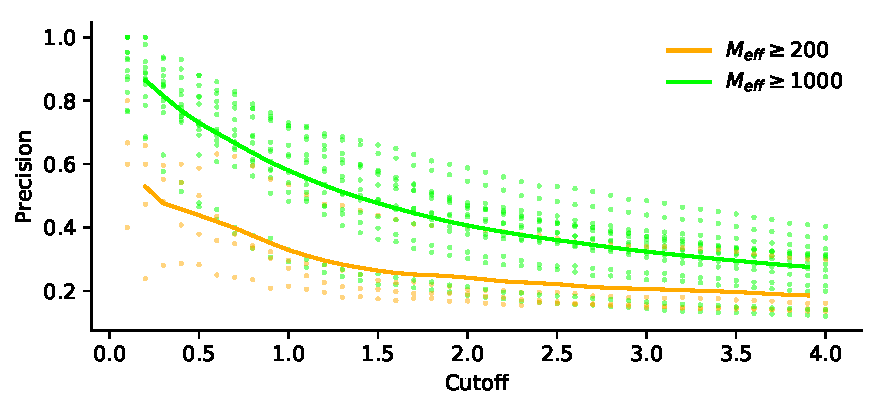
\includegraphics[width=\textwidth]{ample_saint2_conprec.pdf}
    \caption[Contact predicion analysis for numerous contact selection cutoffs]{Contact precision analysis for numerous contact selection cutoffs for targets with alignment depths of more than 200 and more than 1,000 sequences. Lines indicate moving averages for both categories with a window size of three residues. $M_{eff}$ refers to the alignment depth.}
    \label{fig:ample_saint2_conprec}
\end{figure}

\subsection{Comparison of decoy quality}
One main interest of the work presented in this chapter was a direct comparison of the quality of decoys predicted with four \textit{ab initio} structure prediction algorithms. At the time of writing, no such comparison existed on the same dataset, and thus might provide direct insights into the performance of each.

An initial comparison of overall performance highlighted that ROSETTA generated the highest quality decoys (\cref{fig:ample_saint2_tmscoredist}). Across all modelling algorithms the distribution of \gls{tmscore} values is right-skewed, which indicates a higher proportion of non-native-like folds within the sets. A \gls{tmscore} quantile evaluation of each decoy set by algorithm showed that ROSETTA and CONFOLD2 contained only a single set with a lower quantile of less than 0.2 \gls{tmscore} units. In comparison, FRAGFOLD predicted three and SAINT2 eight decoy sets with a lower quantile of less than the aforementioned threshold. In comparison, ROSETTA, CONFOLD2 and FRAGFOLD predicted six, seven and five decoy sets with upper quantiles greater than 0.5 \gls{tmscore} units, whilst SAINT2 predicted zero.

\begin{figure}[H]
    \centering
    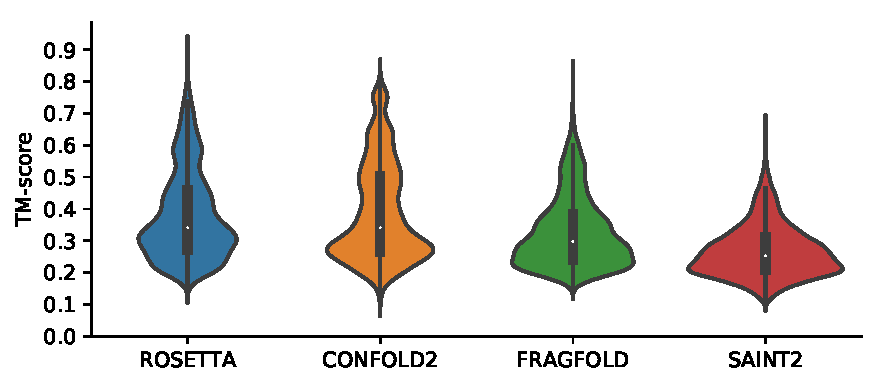
\includegraphics[width=\textwidth]{ample_saint2_tmscoredist.pdf}
    \caption[Distribution of decoy TM-scores for four modelling algorithms]{\gls{kde} of decoy \gls{tmscore} for four different \textit{ab initio} structure prediction algorithms, namely ROSETTA, CONFOLD2, FRAGFOLD and SAINT2. CONFOLD2 contains 9,000 less decoys than the remaining algorithms (for further details refer to \cref{sec:ample_saint2_modelling}).}
    \label{fig:ample_saint2_tmscoredist}
\end{figure}

\begin{figure}[H]
    \centering
    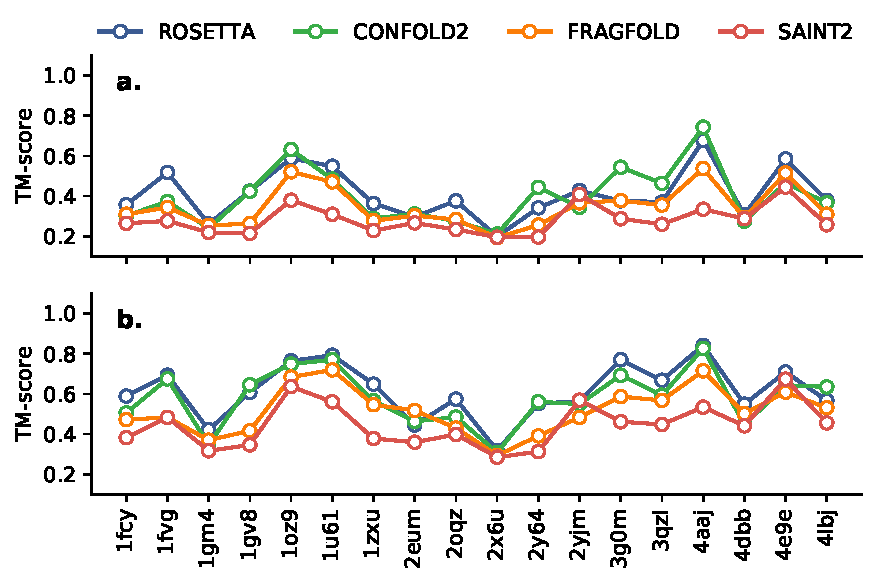
\includegraphics[width=\textwidth]{ample_saint2_tmscoredataincl.pdf}
    \caption[TM-score analysis for four modelling algorithms with contacts]{Per-target \gls{tmscore} analysis for targets modelled with contact information and four separate \textit{ab initio} structure prediction algorithms. Analysis is subdivided by (a) median \gls{tmscore} of all decoys in each set and (b) \gls{tmscore} of the top-1 decoy in each set.}
    \label{fig:ample_saint2_tmscoredataincl}
\end{figure}

A direct comparison of the methods by median \gls{tmscore} of each contact-assisted decoy set reaffirmed ROSETTA's performance in predicting \textit{ab initio} decoys accurately. Across 18 targets, ROSETTA decoy sets contained the best median \gls{tmscore} for 11 targets (CONFOLD2 for remaining seven targets). This was further strengthened when comparing the top-1 decoy for which ROSETTA predicted the best in 13 cases (CONFOLD2 in three cases, FRAGFOLD and SAINT2 in one) (\cref{fig:ample_saint2_tmscoredataincl}).

\textcite{Abriata2018-lu} recently attributed the success in the CASP12 experiment to the improved precision of coevolution-based contact predictions and the availability of many more sequence homologs. Thus, it was of great interest to explore the structure prediction algorithms in this study with regards to their dependence on the availability of sequence homologs and precise contact predictions.

\begin{figure}[H]
    \centering
    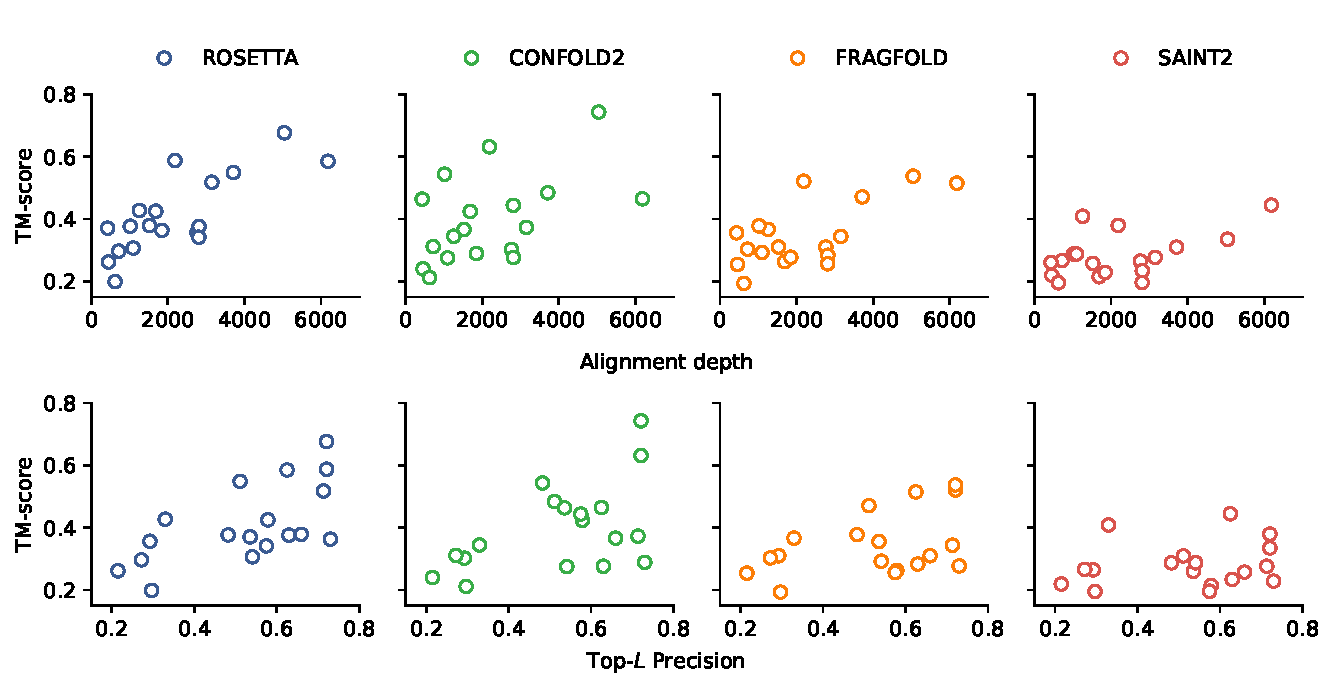
\includegraphics[width=\textwidth]{ample_saint2_neffprectm.pdf}
    \caption[Analysis of alignment depth, precision and TM-scores]{Analysis of median \gls{tmscore} of the contact-based decoy sets and their dependence on  alignment depth and top-$L$ precision.}
    \label{fig:ample_saint2_neffprectm}
\end{figure}

The results obtained in this study further supported the conclusions made by \textcite{Abriata2018-lu} but only for the ROSETTA algorithm. A Spearman's rank-order \gls{cc} analysis of alignment depth and median \gls{tmscore} showed a significant positive correlation for ROSETTA-generated decoy sets (Spearman's $\rho=0.68$, $p<0.01$). This positive correlation was also found for ROSETTA-generated decoy sets with regards to their top-$L$ precision and median \gls{tmscore} (Spearman's $\rho=0.61$, $p<0.01$). All other modelling algorithms did not show a significant correlation, although better decoy sets were generally obtained with greater alignment depths and more precise top-$L$ contacts (\cref{fig:ample_saint2_neffprectm}). Furthermore, the sample size for each correlation analysis was small ($n=18$), and thus further test cases are required for a more confident inference.

Parts of this study also explored the performance of ROSETTA, FRAGFOLD and SAINT2 when no contact prediction was provided as distance restraint information in \textit{ab initio} structure prediction (CONFOLD2 requires contact information, and thus was excluded). ROSETTA performed best for seven of the nine contact-free decoy sets based on median \gls{tmscore} of the entire decoy set and the \gls{tmscore} of the top-1 decoy (\cref{fig:ample_saint2_tmscoredataexcl}). However, the difference was marginal for the majority of cases. The median values for eight ROSETTA and FRAGFOLD decoy sets differed by less than 0.10 \gls{tmscore} units (seven ROSETTA and SAINT2 sets by less than 0.10 units). Furthermore, the top-1 decoys for only three targets differed greatly between the modelling algorithms, whilst the rest was near identical (\cref{fig:ample_saint2_tmscoredataexcl}).

\begin{figure}[H]
    \centering
    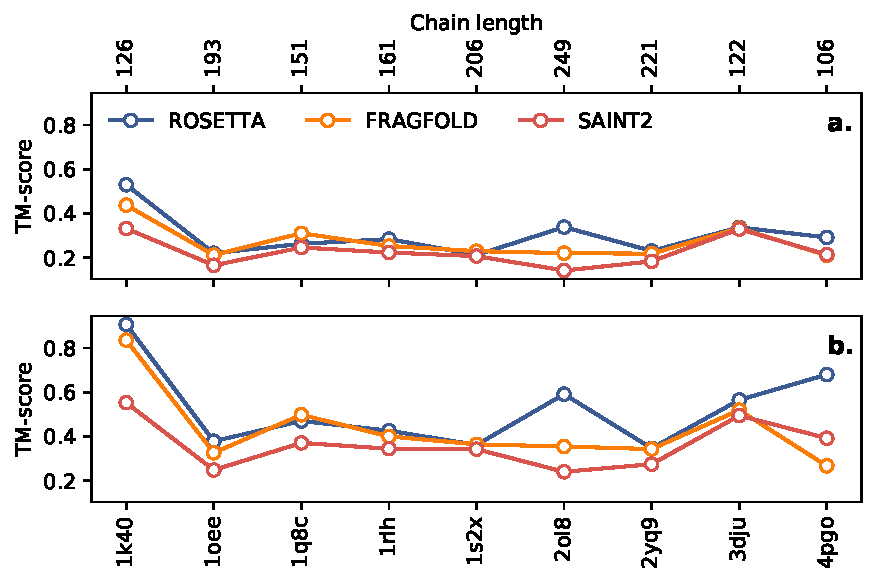
\includegraphics[width=\textwidth]{ample_saint2_tmscoredataexcl.pdf}
    \caption[TM-score analysis for four modelling algorithms]{Per-target \gls{tmscore} analysis for targets modelled without contact information and four separate \textit{ab initio} structure prediction algorithms. Analysis is subdivided by (a) median \gls{tmscore} of all decoys in each set and (b) \gls{tmscore} of the top-1 decoy in each set.}
    \label{fig:ample_saint2_tmscoredataexcl}
\end{figure}

The top decoy predicted by ROSETTA and SAINT2 based on the sequence of the FAT domain of focal adhesion kinase (\gls{pdb} ID: 1k40) differed by 0.35 \gls{tmscore} units. More significantly though, the top-1 decoy predicted by ROSETTA for the outer surface protein A (\gls{pdb} ID: 2ol8) is considered native-like (\gls{tmscore} $=0.59$), whilst the FRAGFOLD (\gls{tmscore} $=0.35$) and SAINT2 (\gls{tmscore} $=0.24$) counterparts predicted incorrect folds. A near-identical scenario applies to the top-1 decoys of the Hypothetical protein PF0907 (\gls{pdb} ID: 4pgo) (ROSETTA \gls{tmscore} $=0.68$; FRAGFOLD \gls{tmscore} $=0.27$; SAINT2 \gls{tmscore} $=0.39$).

\begin{figure}[H]
    \centering
    \includegraphics[width=\textwidth]{ample_saint2_tmfoldsize.pdf}
    \caption[Decoy TM-scores by fold, chain length and algorithm]{Decoy \gls{tmscore}s by fold, chain length and algorithm.}
    \label{fig:ample_saint2_tmfoldsize}
\end{figure}

An analysis of the modelling results by target fold showed that all-\textalpha\ and mixed \textalpha-\textbeta\ target folds were less challenging to predict than all-\textbeta\ targets (\cref{fig:ample_saint2_tmfoldsize}). The multimodal distributions of all-\textalpha\ and mixed \textalpha-\textbeta\ target decoys predicted by ROSETTA spans from 0.10 \gls{tmscore} units to 0.80. In comparison, the approximately normal distribution for all-\textbeta\ targets by the same algorithm centres at 0.32 \gls{tmscore} units (s.d.=0.08 \gls{tmscore} units). Similarly, FRAGFOLD decoys showed a more-spread distribution of decoys for all-\textalpha\ and mixed \textalpha-\textbeta\ decoys compared to all-\textbeta. The \gls{tmscore} distributions for CONFOLD2 mixed \textalpha-\textbeta\ and all-\textbeta\ decoys follow multimodal distributions. Whilst this might indicate that CONFOLD2 either predicted the overall target fold correctly or incorrectly, the data might mislead because of the missing targets in the dataset. Lastly, the distributions of \gls{tmscore} values for either fold class of SAINT2 decoys in \cref{fig:ample_saint2_tmfoldsize} appear more similar than the others indicating less difference between the fold classes. However, similarly to the ROSETTA decoys the all-\textbeta\ distribution appears normal whilst the other two are right-skewed highlighting some more accurate decoys in the overall set (\cref{fig:ample_saint2_tmfoldsize}).

A further subdivision of all target decoys by target chain length was done. At the stage of target selection, three main bins were defined from which targets were randomly sampled (\cref{sec:methods_dataset_predictors}). These bins were defined with target chain length edges of 150 and 200 creating three bins: $0 < n < 150$ \& $150 \leq n < 200$ \& $n \geq 200$ ($n$ refers to the target chain length). A grouping of the decoy \gls{tmscore} by algorithm and target chain length indicated little difference in modelling difficulty (\cref{fig:ample_saint2_tmfoldsize}). The distributions in \cref{fig:ample_saint2_tmfoldsize} show the largest spread across all modelling algorithms for chain lengths in the bin $150 \leq n < 200$. Surprisingly, only FRAGFOLD and SAINT2 performed better for targets in the smallest bin size whilst CONFOLD2 found those targets most challenging. CONFOLD2 also generated the best decoys for one of the largest targets in the dataset (n\textsubscript{res}=216). The set of CONFOLD2 decoys for N-(5-phosphoribosyl)anthranilate isomerase (\gls{pdb} ID: 4aaj) had a median \gls{tmscore} of 0.74. ROSETTA decoys showed a comparable median \gls{tmscore} of 0.68; however, FRAGFOLD (median \gls{tmscore}=0.54) and SAINT2 (median \gls{tmscore}=0.33) were unable to generate decoys of similarly high quality.

\subsection{Molecular Replacement}
The final step in this study was to explore the benefits or drawbacks of each \textit{ab initio} structure prediction algorithm for \gls{mr}.

Each \textit{ab initio} modelling-algorithm generated at least two decoy sets sufficient for \gls{mr} structure solution (\cref{fig:ample_saint2_mrsuccess}). ROSETTA and SAINT2 decoy sets led to the solutions of five targets each, whilst FRAGFOLD decoys solved four and CONFOLD2 decoys just two. All four algorithms predicted decoys of good enough quality to solve the structures of the Hypothetical protein AQ\_1354 (\gls{pdb} ID: 1oz9) and Putative Ribonuclease III (\gls{pdb} ID: 1u61), although SAINT2-based AMPLE search models yielded the highest ratio of successful search models compared to the total trialled in both cases (\cref{fig:ample_saint2_mrsuccess}). Besides these two targets, little consensus exists amongst the targets for which structure solutions were obtained across the different modelling algorithms.

The chain length for targets with structure solutions ranged from 106 (\gls{pdb} ID: 4pgo) to 236 (\gls{pdb} ID: 1fcy) residues. Although statistics cannot reliable indicate the performance with such a small sample size, SAINT2 decoys solved on average the largest targets (mean target chain length ROSETTA=147, CONFOLD2=144, FRAGFOLD=136,  SAINT2=162). The ROSETTA, FRAGFOLD and SAINT2 decoys achieved structure solutions for all three fold classifications, whilst CONFOLD2 decoys did not yield a structure solution for any all-\textbeta\ target. Nevertheless, successful AMPLE ensemble search models for all-\textbeta\ targets derived from the former three algorithms were scarce with only a single one leading to structure solution (\cref{fig:ample_saint2_mrsuccess}).

\begin{figure}[H]
    \centering
    \includegraphics[width=\textwidth]{ample_saint2_mrsuccess.pdf}
    \caption[Summary of MR success with AMPLE ensemble search models]{Summary of MR success with AMPLE ensemble search models. Search models are based on decoy sets generated with different \textit{ab initio} structure prediction protocols. The colour coding indicates structure solution: no solution (red), one solution (orange), more than one solution (green). The number in cells with at least one solution states the percentage of successful search models. The one-letter codes above each column indicate the target fold: all-\textalpha\ (A); all-\textbeta\ (B); mixed \textalpha-\textbeta\ (M). The row labelled ``IDEALH'' refers to AMPLE's ideal helix run.}
    \label{fig:ample_saint2_mrsuccess}
\end{figure}

\begin{figure}[H]
    \centering
    \includegraphics[width=\textwidth]{ample_saint2_tlevelssdist.pdf}
    \caption[Distribution of search model truncation and secondary structure content]{Distribution of (a) search model truncation and (b) secondary structure content for successful AMPLE ensemble search models given decoys from four \textit{ab initio} structure prediction algorithms. Secondary structure for each ensemble search model evaluated with DSSP \cite{Frishman1995-si}.}
    \label{fig:ample_saint2_tlevelssdist}
\end{figure}

The difference in overall decoy quality between the four different \textit{ab initio} structure prediction algorithms was further noticed in the successful AMPLE-generated ensemble search models. ROSETTA decoys resulted in more complete AMPLE ensemble search models, which led to structure solution (\cref{fig:ample_saint2_tlevelssdist}). Although CONFOLD2 had a similar maximum of just under 100\% completeness, 75\% of all successful search models contained at most 40\% of the target sequence. Overall, FRAGFOLD decoys translated into the least complete successful AMPLE search models with 75\% containing less than 20\% of the target sequence. SAINT2 had the shortest range spanning from 8\% to 70\% target completeness.

An inspection of the secondary structure content of all successful ensemble search models outlined an important difference between SAINT2 and the other three modelling algorithms. Successful search models derived from SAINT2 decoys were predominantly \textalpha-helical (\cref{fig:ample_saint2_tlevelssdist}). An analysis of the secondary structure makeup, as assigned by DSSP \cite{Frishman1995-si}, showed that successful SAINT2 search models contained approximately 70-80\% \textalpha-helices with the rest being unassigned secondary structure. In comparison, the successful ensemble search models from other modelling algorithms contained a range from 50-90\% \textalpha-helices, whilst the remainder was either unstructured or \textbeta-structure (\cref{fig:ample_saint2_tlevelssdist}).

This important observation is crucial in assessing the structure solutions obtained since simple helices could be derived from idealised \textalpha-helix libraries, and thus save the great overhead of predicting, preparing and sampling decoys in AMPLE. A visual inspection of SAINT2 ensemble search models highlighted that the FAT domain of focal adhesion kinase (\gls{pdb} ID: 1k40) and the amyloid-\textbeta\ A4 precursor protein-binding family A1 (\gls{pdb} ID: 4dbb) were solved with single \textalpha-helices (\cref{fig:ample_saint2_betaex}). Trialling the experimental data of these targets against AMPLE's ideal helix library \cite{Thomas2015-wu} showed that the former could have been solved without the modelling overhead (\cref{fig:ample_saint2_mrsuccess}). In fact, SAINT2 decoys did not result in any additional structure solutions compared to AMPLE's ideal helix library except for the solution of the A4 precursor protein-binding family A1 (\gls{pdb} ID: 4dbb) (\cref{fig:ample_saint2_mrsuccess}). In comparison, the other modelling algorithms resulted in similar idealised fragments, especially in borderline cases (\cref{fig:ample_saint2_betaex}). However, these fragments were not strictly \textalpha-helical, and thus would require more sophisticated and computationally complex idealised-fragment library generation protocols \cite[e.g.,][]{Jenkins2018-gf} or libraries of recurring tertiary structure motifs \cite[e.g.,][]{Sammito2013-ug}. Nevertheless, even the most sensitive \gls{mr} ideal-fragment-selection algorithms could almost certainly not identify a search model of similar quality to that derived from ROSETTA decoys for the Hypothetical protein PF0907 (\gls{pdb} ID: 4pgo) (\cref{fig:ample_saint2_betaex}), which might be essential in structure solution determination of some targets.

Whilst all \textit{ab initio} structure prediction algorithms enabled structure solutions of at least two targets, the relationship between the quality of the starting decoys and \gls{mr} structure solution success needed to be evaluated. ROSETTA and CONFOLD2 generated the highest quality decoys, followed by FRAGFOLD and SAINT2 (\cref{fig:ample_saint2_tmscoredist}). Thus, most structure solutions would have been expected for the former two since more native-like decoys are generally considered better search models. However, an analysis of the \gls{rmsd} of each ensemble search model's centroid showed that decoy quality may not always be the most reliable indicator. Although search models are often considered suitable once their \gls{rmsd} to the native structure is better than 1.5\AA\ \cite{Scapin2013-yp}, this threshold did not strictly apply to \textit{ab initio} modelling-based AMPLE ensemble search models (\cref{fig:ample_saint2_mrstats}). For example, a small number of SAINT2-derived search models, which were prepared for the FAT domain of focal adhesion kinase (\gls{pdb} ID: 1k40), exceeded this threshold greatly with \gls{rmsd} values $>10$\AA\ (up to 28\AA) yet resulted in PHASER \gls{llg} values in excess of the success threshold of 60 \cite{Oeffner2018-ur}. Additionally, nearly 25\% of all successful ensemble search models had \gls{rmsd} values $\geq2$\AA\ and PHASER \gls{llg} scores of $\geq$60. Although striking at first, structure solutions in these situations were often achieved by out-of-sequence-register placement of search models. An analysis of the \gls{rio} score metric showed that the usefully placed parts of all but one AMPLE search model with \gls{rmsd} value greater than 10\AA\ was out-of-register. Furthermore, it is important to remember that \gls{rmsd} values greatly differ based on the optimal superposition of the model and target.

\begin{figure}[H]
    \centering
    \includegraphics[width=\textwidth]{ample_saint2_betaex.pdf}
    \caption[Examples of PHASER-placed AMPLE search models]{Examples of PHASER-placed AMPLE search models that led to structure solution. AMPLE search models are coloured blue and deposited native structures in grey. The \gls{pdb} identifiers and modelling protocol are provided alongside each example.}
    \label{fig:ample_saint2_betaex}
\end{figure}

Lastly, one characteristic of a good \gls{mr} search model is good stereochemical geometry of its peptide-chain backbone, especially during refinement. Fragment-based structure prediction algorithms typically contained good stereochemistry, because the template fragments are derived from refined protein structures. In comparison, CONFOLD2, which does not use fragments, relies on physics-based energy functions to identify good stereochemistry of the decoy backbone. Thus, it is important to understand if poor stereochemistry was present in CONFOLD2 ensemble search models, such that it might explain why good decoy quality did not translate to more \gls{mr} structure solutions.

\begin{figure}[H]
    \centering
    \includegraphics[width=\textwidth]{ample_saint2_mrstats.png}
    \caption[Relationship between ensemble metrics]{Relationship between ensemble quality, PHASER \gls{llg} and SHELXE \gls{cc}. Data points are coloured based on the outcome of their \gls{mr} trials: green indicate structure solution, red indicate no structure solution.}
    \label{fig:ample_saint2_mrstats}
\end{figure}

\begin{figure}[H]
    \centering
    \includegraphics[width=0.7\textwidth]{ample_saint2_ramach.pdf}
    \caption[Ramachandran outliers of ensemble search model centroids]{Distribution of Ramachandran outliers of AMPLE ensemble search model centroids based on decoys predicted with four \textit{ab initio} structure prediction protocols. Outliers were calculated using PyRAMA (\href{https://github.com/gerdos/PyRAMA}{https://github.com/gerdos/PyRAMA}).}
    \label{fig:ample_saint2_ramach}
\end{figure}

Indeed, a Ramachandran analysis of \textphi\ and \textpsi\ peptide backbone angles outlined much poorer stereochemistry of ensemble search model centroids for CONFOLD2 compared to all fragment-assembly-based structure prediction algorithms (\cref{fig:ample_saint2_ramach}). ROSETTA search models, which were made up of crudely-refined decoys, possessed at most 2\% Ramachandran outliers. SAINT2, which generated less accurate structure predictions compared to other protocols, showed the second best stereochemistry of centroid models without any refinement.  FRAGFOLD contained around 5\% outliers for the majority of search models. In comparison to these statistics CONFOLD2 contained around 5-15\% Ramachandran outliers in centroid decoys. 

Further analysis of the centroids of each truncated AMPLE ensemble demonstrated the importance of good stereochemistry for success. Out of 94 successful ensemble search models only 17 contained outliers. This contrasts to over 390 unsuccessful ensemble search models with \gls{tmscore}s greater than 0.5 units and on average 6\% outliers (min\textsubscript{outliers}=1\%; max\textsubscript{outliers}=23\%). Therefore, perfect peptide backbone stereochemistry is still no guarantee for \gls{mr} structure solution. 

\section{Discussion}
In this chapter, work was conducted to explore \textit{ab initio} protein structure prediction protocols as alternatives to ROSETTA and QUARK. Three algorithms --- CONFOLD2, FRAGFOLD and SAINT2 --- were trialled on a set of 27 globular targets to evaluate their performance with regards to structure prediction and subsequent \gls{mr} trials.

The experiments in this study highlighted that ROSETTA remains the most accurate structure prediction protocol amongst the trialled ones. ROSETTA outperformed the other three algorithms across the majority of protein targets for entire decoy sets and the best decoy in each set. These findings were further confirmed in the latest CASP12 experiments, which outlined ROSETTA's success compared to other protocols \cite{Ovchinnikov2018-wp,Abriata2018-lu}. Furthermore, the findings describing the comparable performance of ROSETTA and CONFOLD2 \cite{Adhikari2018-lj,Michel2017-xh} are supported in this work. Given that the latter relies entirely on the predicted contact information, such performance emphasises the quality and importance of contact prediction in \textit{ab initio} protein structure modelling. It is also to be expected that the increase in sequence availability will improve the decoy quality further \cite{Abriata2018-lu,Schaarschmidt2018-mh}.  
In this study, the alternative fragment-assembly based algorithms FRAGFOLD and SAINT2 were tested. Although both did predict native-like decoys for some targets, their performance was overall much worse than ROSETTA and CONFOLD2. SAINT2 did not generate decoys of native-like quality in cases where all other algorithms did. Beyond overall decoy quality, previous findings suggested a difference in difficulty based on the target fold. These findings are further manifested here. All algorithms predicted most native-like decoys for all-\textalpha\ and mixed \textalpha-\textbeta\ targets. Although previous studies also reported on greater difficulty for larger targets --- especially in cases without contact prediction --- such findings could not be confirmed here.

Given that the application of these decoys is primarily aimed at challenging targets in \gls{mr}, the quality of decoys was not necessarily enough to predict the success of AMPLE-generated search models. The results in this chapter clearly demonstrated that highly accurate decoys predicted by CONFOLD2 do not routinely translate into MR structure solutions. Despite a recent example of the successful application of \gls{cns}-generated decoys in \gls{mr} \cite{Sjodt2018-zq}, further research is required to identify the main bottleneck observed in this study. ROSETTA, FRAGFOLD and SAINT2 achieved structure solutions for a number of targets, despite poor decoy quality in cases of the latter two. CONFOLD2 decoys appear to suffer from poor stereochemistry, and results suggest that decoy refinement might be essential to exploit the underlying decoy quality \cite{Mao2014-lg}.

In conclusion, ROSETTA remains the best modelling algorithm for unconventional \gls{mr} in AMPLE. Although some of this success must be due to the fact that AMPLE's algorithm is tailored towards exploiting the cluster variance derived from ROSETTA decoys, it cannot be downplayed that ROSETTA generates the most accurate decoys overall. However, it is crucial to investigate whether CONFOLD2 decoys, potentially remodelled to improve the backbone stereochemistry, might provide a suitable routine alternative to ROSETTA, especially because fragment databases are not required and modelling time per decoy is reduced by approximately a factor of four.


\chapter{Decoy subselection using contact information to enhance MR search model creation} \label{chap:ample_decoys}
\clearpage
% \chapter{Decoy subselection to enhance MR search model creation} \label{chap:ample_decoys}
\clearpage

\section{Introduction}
Work presented in \cref{chap:proof_of_principle,chap:rosetta_energy_functions,chap:alternate_abinitio_protocols} highlighted the much improved decoy quality achievable by restraining the conformational search space in template-free protein structure prediction with residue-residue contacts. Furthermore, the data also highlighted that this improvement extends AMPLE's performance of achieving structure solution for more challenging targets. However, the data in \cref{chap:rosetta_energy_functions,chap:alternate_abinitio_protocols} also indicated that AMPLE's protocol is currently not tailored towards decoy sets with much improved accuracy. In some cases, decoy sets with correctly predicted folds --- whereby the mean \gls{tmscore} of the decoy set was greater than 0.5 score units --- did not generate any successful ensemble search models.

Furthermore, decoy similarity to the crystal structure was exceptionally high in some cases (\gls{rmsd} $<1.5$\AA). Although challenging by current means to identify these decoys, it is of great interest to structural biologists to do so since these decoys might be sufficient by themselves as \gls{mr} search models. A contact prediction, which is typically used to restrain the folding protocol, might provide enough information to drive such identification. Indeed, \textcite{Kosciolek2014-bt} and \textcite{De_Oliveira2016-gj} highlighted the usefulness of long-range residue-residue contact pair satisfaction for model selection since it correlates well with decoy quality. Additionally, \textcite{Adhikari2018-lj} use long-range contact satisfaction routinely in CONFOLD2 to exclude the worst decoys amongst the set predicted ones.

Thus, this chapter focused on exploring alternative strategies of decoy selection in AMPLE. In particular, work presented here focused on exploiting long-range contact information to drive search model generation to extend AMPLE's performance on difficult cases further.

\section{Materials \& Methods}
\subsection{Target selection}
The dataset for this study consisted of 113 ROSETTA decoy sets generated throughout the work outlined in \cref{chap:proof_of_principle,chap:rosetta_energy_functions,chap:alternate_abinitio_protocols}. The 113 decoy sets covered all targets in the ORIGINAL (\cref{table:appendix_dataset_original}), PREDICTORS (\cref{table:appendix_dataset_predictors}) and TRANSMEMBRANE (\cref{table:appendix_dataset_transmembrane}) datasets. Top-$L$ ($>5$ residues sequence separation) CCMPRED \cite{Seemayer2014-zp}, PCONSC2 \cite{Skwark2014-qp}, METAPSICOV STAGE1 \cite{Jones2015-vq} and MEMBRAIN \cite{Yang2013-bf} contact pairs were used in combination with the \textit{FADE} energy function to restrain the template-free structure prediction process.

\subsection{Computation of range-specific satisfaction scores}
The satisfaction of short- ($>5$ residues sequence separation), medium- ($>12$ residues sequence separation) and long-range contact pairs ($>23$ residues sequence separation) were computed for each decoy in each set (for further details, see \cref{sec:methods_longrange_satisfaction}). Hereby, the short-, medium- or long-range predicted contacts were extracted from the original predictions used to restrain the template-free structure prediction, matched against the contact pairs observed in individual decoys and the range-specific contact satisfaction score evaluated. 

\subsection{Decoy subselection} \label{sec:ample_decoys_decoy_selection}
Each set of decoys was ranked in descending order by their long-range contact pair satisfaction scores and the $n$ decoys with the lowest scores removed from each set. The number of decoys to remove $n$ was selected using a number of different strategies:

\begin{description}[style=multiline,leftmargin=4cm]
    \item[\textit{NONE}] leave the original set unchanged
    \item[\textit{LINEAR}] remove the worst 500 decoys
    \item[\textit{CUTOFF}] remove all decoys with a score of $<0.287$ 
    \item[\textit{SCALED}] remove all decoys with a scaled score of $<0.5$, where the scaled score is score divided by set average
    \item[\textit{INDIVIDUAL}] keep the top-5 decoys only
\end{description}

The fixed definition in the \textit{CUTOFF} strategy was determined by \textcite{De_Oliveira2016-gj}. The scaled score used by the \textit{SCALED} strategy was computed by dividing each decoy's long-range contact pair satisfaction by the set's average.

The \textit{INDIVIDUAL} subselection strategy differed substantially from the others. The top-5 decoys by long-range contact satisfaction were selected and subjected to treatment outside of AMPLE. The per-decoy treatments were the following:

\begin{description}[style=multiline,leftmargin=4cm]
    \item[default] leave the decoy unchanged
    \item[domain] remove all residues with $kde<\frac{1}{2}max_{kde}$, where $kde$ corresponds to the \gls{kde} and $max_{kde}$ to the maximum \gls{kde} obtained by applying the algorithm described by \textcite{Sadowski2013-zu} to the top-5$L$ contact map
    \item[dssp] remove all residues with secondary structure of ``helix turn (T)'', ``bend (S)'' or ``coil (C)'', which were assigned using DSSP \cite{Frishman1995-si} 
    \item[fragment] remove all residues that do not satisfy the following condition: extract all contacts from a decoy [C\textbeta\ distance of $<8$\AA\ (C\textalpha\ in case of Gly)] and reconstruct the decoy's sequence using the residue indices present in the set of contacts, then keep residues that are within a sequence fragment of at least three consecutive residues
    \item[variance] remove all residues with variance of more than 5\AA\textsuperscript{2}, which was extracted from the decoy's corresponding cluster in the \textit{NONE} subselection strategy
\end{description}

\subsection{Molecular Replacement} \label{subsec:ample_decoys_methods_mr}
To evaluate the benefits of such subselection to \gls{mr} in AMPLE, a subset of 35 decoy sets (spanning 35 unique targets) were processed as described in \cref{sec:ample_decoys_decoy_selection} and subjected to AMPLE v1.2.0 and CCP4 v7.0.28. Default options were chosen with the following exceptions: decoys in all 10 clusters were used, subcluster radii thresholds were set to 1 and 3\AA, and side-chain treatments were set to \texttt{polyala} only. This change in protocol from AMPLE's initial mode of operation \cite{Bibby2012-lm} was shown to be advantageous in most cases by \textcite{Thomas2017-qu}, and thus trialled in this context. 

To allow comparability of these results to previous AMPLE runs, an additional condition was added, namely \textit{NONE\_classic}. The decoy set from the \textit{NONE} strategy was thereby subjected to the AMPLE protocol with default settings except \texttt{-num\_clusters}, which was set to sample the three largest clusters. Thus, the \textit{NONE\_classic} strategy differed from the \textit{NONE} one in three aspects: top-3 clusters are used instead of top-10, 1, 2 and 3\AA\ subclustering radii are used instead of 1 and 3\AA\ only, and the most-reliable and all-atom side-chain treatments are kept.

All individual decoys created under the \textit{INDIVIDUAL} strategy were subjected as poly-alanine decoys to MRBUMP v0.9 \cite{Keegan2018-kn} with identical settings to those used in AMPLE. 

Each \gls{mr} run was assessed using the criteria defined in \cref{sec:methods_mr_success}.

\section{Results}
This chapter focused on identifying further uses of predicted residue-residue contact pairs in unconventional \gls{mr}. In particular, the exclusion of template-free structure prediction decoys by their contact satisfaction scores was investigated. A total of 113 decoy datasets were used to identify potential means of identifying the best or worst decoys. Furthermore, three strategies were trialled alongside two standard approaches to test the consequences of excluding the worst decoys in ensemble search model preparation in AMPLE.

\subsection{Contact pair satisfaction correlates with decoy quality} \label{subsec:ample_saint2_concorr}
\textcite{Kosciolek2014-bt} previously identified a correlation between the \gls{tmscore} of a decoy and its fraction of satisfied contact pairs. Although reporting striking positive correlations (short-range:$\rho=0.50$; medium-range:$\rho=0.57$; long-range: $\rho=0.87$) for top-1 decoys, the study by \textcite{Kosciolek2014-bt} was limited to 10 representative targets with a maximum chain length of 158 residues. Furthermore, FRAGFOLD \cite{Jones2001-mc} was used for template-free protein structure prediction, a method with inferior performance to ROSETTA \cite{Rohl2004-dj} when using the decoys in unconventional \gls{mr} (see \cref{chap:alternate_abinitio_protocols}). Thus, the more diverse set of decoys generated in this study might be more representative in determining a correlation between decoy \gls{tmscore}s and contact pair satisfaction.

\begin{table}[H]
  \centering
  \caption[Correlation analysis between decoy TM-score and contact satisfaction]{Pearson's \gls{cc} analysis between a ROSETTA decoy's \gls{tmscore} and short-, medium- and long-range contact satisfaction. Probability values for all $\rho$ coefficients are $<0.01$.}
  \label{table:ample_decoys_tmscore_consat}
  \begin{tabularx}{\textwidth}{X X X X}
      \hline
      \multirow{2}{*}{\textbf{Target class}} & \multicolumn{3}{c}{\textbf{Pearson's \gls{cc}}} \\ \cline{2-4}
      & Short-range   & Medium-range  & Long-range \\
      \hline
      all                               & 0.11          & 0.18          & 0.64 \\
      all-\textalpha                    & 0.30          & 0.44          & 0.69 \\
      all-\textbeta                     & 0.40          & 0.54          & 0.50 \\
      mixed \textalpha-\textbeta        & 0.42          & 0.55          & 0.69 \\
      transmembrane                     & 0.08          & 0.48          & 0.70 \\
      \hline
  \end{tabularx}
\end{table}

A Pearson's \gls{cc} analysis with 113 ROSETTA decoy sets representing 56 globular and transmembrane targets showed positive linear correlations between a decoy's \gls{tmscore} and short-, medium- and long-range contact satisfaction (\cref{table:ample_decoys_tmscore_consat}). Furthermore, separating the correlation analysis of all targets by fold classification revealed that all-\textalpha, mixed \textalpha-\textbeta\ and transmembrane protein targets showed the strongest positive correlations for long-range contact satisfaction (\cref{table:ample_decoys_tmscore_consat}). All-\textbeta\ and mixed \textalpha-\textbeta\ decoy sets showed the strongest correlations for short- and medium-range contact satisfaction, whereby the former highlighted a stronger positive correlation between the decoy's \gls{tmscore} and its medium-range contact satisfaction than its long-range contact satisfaction (medium-range:$\rho=0.54$; long-range:$\rho=0.50$) (\cref{table:ample_decoys_tmscore_consat}). Notably, the decoys of transmembrane protein targets showed no significant correlation between \gls{tmscore} and short-range contact satisfaction ($\rho=0.08$; \cref{table:ample_decoys_tmscore_consat}). However, it is worth noting that some targets may be represented by more than one decoy set restrained during folding with a unique set of restraints. Thus, the combination of independent template-free modelling runs alongside independently obtained contact predictions for the same targets warrants above analysis to be valid.

Following on from the Pearson's \gls{cc} analysis, a linear regression model was fitted to individual subsets of the data used for the correlation analysis to see if a decoy's \gls{tmscore} could be predicted from its contact satisfaction score. However, weak coefficients of determination indicated that only some cases show models with reasonably good fits to the data (\cref{fig:ample_decoys_smlrcstmfold}). Nevertheless, all models further supported the positive linear correlations between a decoy's \gls{tmscore} and its range-dependent contact satisfaction. Interestingly, the strongest and best fits of the linear regression model to its corresponding data was for long-range contact pairs, where the linear regression models were also near identical between the different fold categories (\cref{fig:ample_decoys_smlrcstmfold}).

\begin{figure}[H]
	\centering
	\includegraphics[width=\textwidth]{ample_decoys_smlrcstmfold.pdf}
        \caption[Regression model between decoy TM-score and contact satisfaction]{Linear regression model fitted to decoy \gls{tmscore}s and corresponding fractions of satisfied, range-dependent contacts. Targets were further separated by fold classification. Coefficients of determination ($R^2$-values) added alongside each regression model.}
	\label{fig:ample_decoys_smlrcstmfold}
\end{figure}

An analysis of the correlation between the \gls{tmscore} and long-range contact satisfaction of individual decoy sets further highlighted the potential to subselect decoy sets by their long-range contact satisfaction. One hundred and eight decoy sets showed statistically significant positive correlations between decoy \gls{tmscore}s and their long-range contact satisfaction ($\rho$-values in range of 0.09 to 0.97 with p-value $<0.01$). A single ROSETTA decoy set, derived for the glycolipid transfer protein (\gls{pdb} ID: 2eum) and restrained with predicted METAPSICOV STAGE1 contact data, showed a weak negative correlation ($\rho=-0.10$, $p<0.01$). The remaining four decoy sets, derived for targets with \gls{pdb} IDs 1chd, 1gm4, 2x6u and 3ouf and restrained with predicted METAPSICOV STAGE1 contact data except for 2x6u (PCONSC2), showed no statistically significant correlation between the \gls{tmscore} and long-range contact satisfaction of the decoy sets. 

A further subdivide of the previously presented data by metapredictor highlighted that no predictor outperformed the others. Decoy sets calculated using predictions from all metapredictors exhibited a range of stronger to weaker correlations. Similarly, target chain length and fold did not show overall stronger or weaker correlations. 

So far, all analyses focused on entire sets of decoys (1,000 decoys per set); however, it is often desirable to know if one could better estimate the accuracy of the best decoy by some measure. \textcite{Kosciolek2014-bt} demonstrated strong positive correlations for short-, medium- and long-range contact satisfaction with a decoy's corresponding \gls{tmscore} (short-range:$\rho=0.50$; medium-range:$\rho=0.57$; long-range: $\rho=0.87$). In this work, some of these findings were confirmed (short-range: no correlation; medium-range:$\rho=0.52$; long-range:$\rho=0.69$) although the strength of the correlation for long-range contact satisfaction is much weaker than previously observed (\cref{fig:ample_decoys_smlrcstmtop1}). The weak positive correlation for short-range contact satisfaction is statistically non-significant, and thus could not be validated. 

\begin{figure}[H]
	\centering
        \includegraphics[width=\textwidth]{ample_decoys_smlrcstmtop1.pdf}
        \caption[Top-1 decoy TM-score and contact satisfaction analysis]{Analysis of the relationship between \gls{tmscore} and contact satisfaction for the top-1 decoy (as ranked by \gls{tmscore}) in each decoy set.}
	\label{fig:ample_decoys_smlrcstmtop1}
\end{figure}

\subsection{Long-range contact satisfaction metric to filter decoy sets}
In \cref{subsec:ample_saint2_concorr}, the data highlighted that decoy quality correlates positively with contact satisfaction. In particular, a strong positive correlation between long-range contact satisfaction and decoy quality could be established for almost all decoy sets in this study. A key ambition in this work was to determine if this correlation could be used to alter the starting decoy sets prior to the submission to the AMPLE cluster-and-truncate pipeline to enhance the chances of generating ensemble search models for more frequent \gls{mr} success.

The difference in mean \gls{tmscore} of each decoy set before and after applying a subselection strategy (see \cref{sec:ample_decoys_decoy_selection}) is shown in \cref{fig:ample_decoys_deltatmsub}. Estimating a decoy's quality by short-range contact satisfaction resulted in marginal mean \gls{tmscore} changes of decoy sets ($\Delta_{CUTOFF}=-0.003$; $\Delta_{LINEAR}=0.008$; $\Delta_{SCALED}=0.001$). In comparison, medium- ($\Delta_{CUTOFF}=0.005$; $\Delta_{LINEAR}=0.015$; $\Delta_{SCALED}=0.002$) and especially long-range ($\Delta_{CUTOFF}=0.025$; $\Delta_{LINEAR}=0.032$; $\Delta_{SCALED}=0.005$) contact satisfaction were better metrics to use to improve the mean \gls{tmscore}s of each decoy set. Notably, per-decoy long-range contact satisfaction provided the best estimate for identifying and excluding the least accurate decoys independent of the subselection strategy. 

\begin{figure}[H]
	\centering
	\includegraphics[width=\textwidth]{ample_decoys_deltatmsub.pdf}
        \caption[TM-score comparison pre- and post-decoy subselection]{Differences in mean \gls{tmscore} for decoy sets pre- and post-decoy subselection. Each subselection strategy is stated in each subplot along with the contact range used to establish decoy inclusion in the final set. Green bars indicate \gls{tmscore} changes in favour of subselected decoy sets, red in favour of complete ones.}
	\label{fig:ample_decoys_deltatmsub}
\end{figure}

Given the improvement of \gls{tmscore}s for each decoy set by decoy subselection, it was important to analyse the number of decoys left in each set after long-range contact-satisfaction subselection. This metric is important since too few decoys might not generate any AMPLE ensemble search models due to AMPLE's filters after clustering and sub-clustering. For the decoy sets used in this study, the \textit{LINEAR} strategy removed on average the most decoys from each set with a fixed number of 500 (median=500). In comparison, the \textit{CUTOFF} subselection strategy removed on average 409 decoys (median=316) whilst the \textit{SCALED} method only 56 (median=29). However, the sample-dependent strategies (\textit{CUTOFF} and \textit{SCALED}) may remove a much greater number of decoys from a set if the corresponding satisfaction scores fall below a certain threshold (maximum removed by \textit{CUTOFF}=1000 and \textit{SCALED}=497). Since these numbers varied drastically similarly to the changes in \gls{tmscore}, it became apparent that the more decoys were removed, the better the overall score became, which further supported the linear correlation between long-range contact satisfaction and \gls{tmscore}.

In certain cases, some subselection strategies greatly altered the overall size and quality of the resulting decoy set, which started with a set of 1,000 decoys. The METAPSICOV STAGE1 decoy set of the ankyrin sequence (\gls{pdb} ID: 2qyj) showed overall quality improvements from 0.006 (short-range \textit{SCALED}; $n_{models}=958$) to 0.213 (long-range \textit{CUTOFF}; $n_{models}=218$). The CCMPRED decoy set of sensory rhodopsin II sequence (\gls{pdb} ID: 1gu8) showed overall changes from -0.155 (short-range \textit{CUTOFF}; $n_{models}=2$) to 0.06 (long-range \textit{LINEAR}; $n_{models}=500$).

Overall, the optimal strategy to select or exclude decoys from a starting set of structures appeared to be long-range contact satisfaction driving the \textit{LINEAR} strategy.

\subsection{AMPLE's cluster-and-truncate approach with filtered decoy sets}
For evaluation of performance of filtered decoy sets in \gls{mr}, a smaller sample of 35 decoy sets was selected spanning 35 unique targets (21 globular and 14 transmembrane targets). The contact prediction algorithm generating the restraints for the template-free structure predictions was PCONSC2 (globular targets) or CCMPRED (transmembrane targets). Each decoy set was subjected to the AMPLE pipeline with certain decoys removed according to one of four subselection strategies, namely \textit{NONE}, \textit{CUTOFF}, \textit{LINEAR} and \textit{SCALED}.

The initial step in the AMPLE pipeline is the clustering of decoys. A comparison of SPICKER clusters between the \textit{NONE} default strategy and the \textit{CUTOFF}, \textit{LINEAR} and \textit{SCALED} subselection strategies highlighted an important observation. Larger clusters --- those ranked higher --- showed higher similarity between a subselection strategy and the default (\cref{fig:ample_decoys_jaccluster}). The top SPICKER cluster showed high similarities between the \textit{NONE} strategy and all other subselection ones, whereby it has to be noted that the \textit{LINEAR} strategy contained only 50\% of the starting decoys, and thus can at best show a Jaccard index of 0.5. With increasing cluster index, the overall similarity degraded and most of the decoys in cluster 10 were non-identical between each subselection strategy and the default. It is important to consider though that clusters might be swapped between subselection strategies, and thus the Jaccard index might not reliably indicate presence of individual decoys.

Furthermore, a similar analysis to compare the overall quality of each cluster to the target structure revealed less difference between the default and each subselection strategy for higher-ranked SPICKER clusters (\cref{fig:ample_decoys_tmcluster}). With decreasing SPICKER cluster index, the difference in median \gls{tmscore}s started to alternate without any particular pattern. Thus, pre-selecting decoys prior to AMPLE's cluster-and-truncate approach most certainly preserved the top cluster for the \textit{CUTOFF} and \textit{SCALED} subselection strategies, whereby lower clusters showed more deviation from the default.

\begin{figure}[H]
    \centering
    \begin{subfigure}[b]{\textwidth}
        \includegraphics[width=\textwidth]{ample_decoys_jaccluster.pdf}
        \caption{}
        \label{fig:ample_decoys_jaccluster}
    \end{subfigure}
\end{figure}

\begin{figure}[H]\ContinuedFloat
    \begin{subfigure}[b]{\textwidth}
        \includegraphics[width=\textwidth]{ample_decoys_tmcluster.pdf}
        \caption{}
        \label{fig:ample_decoys_tmcluster}
    \end{subfigure}
    \caption[Effect of decoy subselection on SPICKER clusters]{Effect of decoy subselection on SPICKER clusters. Effect illustrated by (a) the Jaccard Index and (b) median \gls{tmscore} difference. Values were calculated for clusters resulting from the full starting set of decoys and the \textit{CUTOFF}, \textit{LINEAR} and \textit{SCALED} subselection strategies. Larger \gls{tmscore} differences indicate that the subselection improved the \gls{tmscore} of the cluster.}
\end{figure}

The mean of the inter-decoy variance computed by THESEUS --- used in AMPLE to guide truncation of each cluster --- is reduced in lower clusters compared to the \textit{NONE} default strategy (\cref{fig:ample_decoys_vardeltacluster}). In other words, these clusters have become more structurally homogeneous. The clusters of decoys based on the galectin-3 domain (\gls{pdb} ID: 1kjl) sequence show overall the highest reduction in mean inter-decoy variance up to -15\AA\textsuperscript{2} compared to the default strategy. Similarly, clusters 4 and 8 of the K\textsuperscript{+}-channel protein domain (\gls{pdb} ID: 3ouf) show reductions in mean inter-decoy variance of up to -20\AA\textsuperscript{2}. In general, clusters starting from \textit{CUTOFF}-subselected decoys show the greatest mean inter-decoy variance reductions, followed by \textit{LINEAR} and then \textit{SCALED}-subselected decoys sets.

A comparison of intermediate stages in the AMPLE pipeline resulting from differently subselected decoy sets is generally very difficult. Each strategy resulted in different starting sets, which resulted in different clusters. Since AMPLE's objective truncation procedure was based on the inter-decoy variance, it might be greatly affected by differing clusters. Nevertheless, structure solution is more likely when AMPLE generated more ensemble search models because a greater number of search models reflects greater inter-cluster decoy similarity and trialling a greater number should provide a higher chance of success. A count of generated AMPLE ensemble search models revealed that the \textit{SCALED} strategy generated the most search models ($n=7,611$), which is roughly 300 more than the default \textit{NONE} strategy ($n=7,340$). The \textit{CUTOFF} subselection strategy generated the least ensemble search models ($n=7,237$), whilst the \textit{LINEAR} strategy's count ($n=7,401$) was very similar to the \textit{NONE} one.

\begin{figure}[H]
    \centering
    \includegraphics[width=\textwidth]{ample_decoys_vardeltacluster.pdf}
    \caption[Effect of decoy subselection on THESEUS variance]{Effect of decoy subselection on mean inter-decoy THESEUS variance. Difference in mean variance calculated between the default and the three decoy subselection strategies \textit{CUTOFF}, \textit{LINEAR} and \textit{SCALED}. Data for clusters 1, 5 and 10 shown as examples.}
    \label{fig:ample_decoys_vardeltacluster}
\end{figure}

Further inspection of the number of AMPLE ensemble search models by target revealed near identical numbers between the \textit{NONE}, \textit{LINEAR} and \textit{SCALED} strategies (\cref{fig:ample_decoys_mrsuccesstarget}). In fact, only few outliers for each of those methods distinguished them from the others. The \textit{CUTOFF} strategy showed greater deviation from the other three, especially for certain targets with differences up to approximately 200 ensemble search models (\cref{fig:ample_decoys_mrsuccesstarget}). A comparison of all these strategies to the previous default processing in AMPLE (\textit{NONE\_classic}; further details in \cref{subsec:ample_decoys_methods_mr}) highlighted a reduction in the total number of generated ensemble search model count (\cref{fig:ample_decoys_mrsuccesstarget}). A comparison of the previous default (\textit{NONE\_classic}) with the new one (\textit{NONE}) showed on average 144 fewer ensemble search models per target, whilst sampling a larger range of folds through all ten clusters.

\subsection{MR search models by processing single decoys}
In addition to the decoy set subselection, this study also attempted to identify single decoys of sufficient quality to be used directly as \gls{mr} search models. Although ensembles are generally more desirable \gls{mr} search models \cite{Rigden2018-zt,Keegan2018-kn,Thomas2015-wu}, individual decoys might be successful by themselves, and thus save the overhead of generating and trialling a great number of AMPLE ensemble search models. Thus, the top-5 decoys, as judged by long-range contact satisfaction, were selected from each decoy set. Four distinct processing approaches were applied to each decoy to eliminate less reliable parts, and subsequently compared against the unmodified initial decoy.

\begin{figure}[H]
	\centering
	\includegraphics[width=\textwidth]{ample_decoys_individualinitial.pdf}
        \caption[Selection of single decoys by long-range satisfaction]{Analysis of long-range contact-satisfaction-based decoys with respect to the relationship between (a) the satisfaction and decoy quality and (b) the quality compared to the remaining, excluded decoy set.}
	\label{fig:ample_decoys_individualinitial}
\end{figure}

The correlation between a decoy's long-range contact satisfaction and its \gls{tmscore} has previously been outlined and was further confirmed here (\cref{fig:ample_decoys_individualinitial}). However, the positive correlation was dependent on the target's fold class and the overall accuracy of the decoy set. An analysis of the top-5 decoys by long-range contact satisfaction in each decoy set showed that 50\% of selected decoys fall in the 80\textsuperscript{th} percentile or greater of \gls{tmscore}s in each decoy set whilst 90\% are in at least the 40\textsuperscript{th} percentile (\cref{fig:ample_decoys_individualinitial}).

A comparison of \gls{rmsd} value changes indicated that the ``fragment'' and ``variance'' metrics provided the best approximation to identifying less-reliable regions in each decoy. The average \gls{rmsd} change compared to the original decoys was just under 4.0\AA. This compared to a slightly lower \gls{rmsd} change of 2.1\AA\ for ``DSSP''-treated decoys and 1.5\AA\ for the ``domain'' treatment. Although almost all decoys were improved by either of the treatments, a small number of decoys worsened in terms of \gls{rmsd} compared to its native structure. All treatments except the ``fragment'' one had worsened decoys in the final set, with changes up to -1.6\AA. 

A comparison of the range of \gls{rmsd} values revealed much greater changes for the ``fragment'' and ``variance'' conditions (\cref{fig:ample_decoys_individualrmsd}). However, these changes were not reflected in the fraction of residues retained in each decoy. Most residues were removed by the ``domain'' treatment (\textmu=61.6\%), whilst the ``fragment'' one saw the least removal (\textmu=34.5\%). Similarly to the ranged in \gls{rmsd} values, the ``fragment'' and ``variance'' treatments resulted in the greatest spread of fraction of residues in the treated decoy. The values range for both treatments from retaining less than 5\% of the initial decoy up to 100\%.

\begin{figure}[H]
	\centering
	\includegraphics[width=\textwidth]{ample_decoys_individualrmsd.pdf}
        \caption[Difference in RMSD for individually processed decoys]{Distribution of differences in \gls{rmsd} values between the initial and modified decoys under four different treatments. A positive \textDelta\textsubscript{RMSD} value corresponds to a decrease in \gls{rmsd} compared to the crystal structure.}
	\label{fig:ample_decoys_individualrmsd}
\end{figure}

A further aspect of the decoy treatments highlighted that the fraction of residues retained after decoy post-processing correlates with the cluster variance of the decoy, which were extracted from THESEUS results of each decoy's cluster in the \textit{NONE} strategy (\cref{fig:ample_decoys_individualcorrtm}). Unlike the variance metric, all other processing metrics did not show a correlation with the fraction of residues retained. This explains at least in part why much greater changes in \gls{rmsd} value between the initial and processed decoy were observed for the ``variance'' treatment compared to the others. However, if a decoy was of particularly poor quality (\gls{tmscore} $<0.3$), the ``variance'' treatment retained as little as 0.87\% and 1.7\% of the initial decoy (2 and 4 residues) whilst the others retained a much larger fraction of at least 40\% for equivalent decoys.

\begin{figure}[H]
        \centering
        \includegraphics[width=\textwidth]{ample_decoys_individualcorrtm.pdf}
        \caption[Relationship between decoy quality and fraction of residues retained]{Scatter plots of initial decoy \gls{tmscore} and the fraction of residues retained after one of four different residue removal treatments.}
        \label{fig:ample_decoys_individualcorrtm}
\end{figure}

\subsection{Decoy subselection extends AMPLE's performance}
The final step in this study was the assessment of AMPLE ensemble search models and single-decoy-based search models in \gls{mr}. In particular, the comparison of different decoy subselection strategies and individual decoy-processing treatments was of great interest since it might extend AMPLE's performance beyond that described in \cref{chap:proof_of_principle,chap:rosetta_energy_functions,chap:alternate_abinitio_protocols}.

A comparison of the total number of targets solved by each subselection strategy showed that the \textit{CUTOFF}-subselected decoys led to most structure solutions (14 out of 35) (\cref{fig:ample_decoys_mrsuccesstarget}). Although slightly less successful, the \textit{LINEAR} and \textit{SCALED} subselection strategies led to structure solutions of two additional targets compared to the \textit{NONE} strategy (11 out of 35). The \textit{LINEAR} and \textit{SCALED} strategies were on par with AMPLE's default, the \textit{NONE\_classic} strategy (\cref{fig:ample_decoys_mrsuccesstarget}). Although the \textit{NONE\_classic} strategy generated two version of each ensemble search model with poly-alanine and all-atom side chain treatments, the former was enough to solve all targets (\cref{fig:ample_decoys_mrsuccesstarget}). Therefore, the \textit{LINEAR} and \textit{SCALED} subselection strategies would be the minimum processing requirement to solve the same number of targets with fewer search models and hence improved performance.

\begin{figure}[H]
    \centering
    \includegraphics[width=\textwidth]{ample_decoys_mrsuccesstarget.pdf}
    \caption[Molecular Replacement summary of decoy-subselected ensembles]{Molecular Replacement summary of decoy-subselected AMPLE ensembles. AMPLE-generated ensemble counts illustrated at the top with Molecular Replacement results in grid below: red cell equates to no solution; orange to a singleton solution; and green to multiple solutions. All \textit{INDIVIDUAL} attempts were compressed to a single row per decoy set. The number in the orange and green cells indicates the percentage of ensemble search models leading to structure solutions. One letter code above each column indicates the target fold: ``T'' for transmembrane; ``A'' for all-\textalpha; ``B'' for all=\textbeta; ``M'' for mixed \textalpha-\textbeta. Values alongside each row indicate the number of targets with structure solutions and total number targets attempted. Targets are sorted from left to right with increasing median \gls{tmscore} of the starting decoy set. The black lines highlight \gls{tmscore} thresholds from 0.3 to 0.7 from left to right. The subselection strategy \textit{IDEALH} refers AMPLE's ideal helix library.}
    \label{fig:ample_decoys_mrsuccesstarget}
\end{figure}

The \textit{CUTOFF} method yielded the highest number of structure solutions based on AMPLE ensemble search models whilst generating the fewest search models. In fact, this subselection strategy generated no ensemble search models for target 2bhw. Furthermore, the \textit{CUTOFF} method achieved amongst the best ratio of search models leading to structure solution compared to the total number produced. 

In few cases, only a single AMPLE search model led to a structure solution (orange cells in \cref{fig:ample_decoys_mrsuccesstarget}). Upon closer inspection, 71\% of all singleton solutions were achieved with AMPLE ensemble search models containing at least 30\% of the target sequence. Twenty-nine percent of the singleton solutions contained at least 50\% of the target sequence, whilst none contained more than 70\%. Three out of four search models with less than 30\% of the target sequence were derived from the PCONSC2 decoy set predicted for the ketosteroid transcriptional regulator KstR2 (\gls{pdb} ID: 4w97) sequence and contained one, two or three small helical fragments.  

In certain cases the subselection of starting decoys made a subtle yet essential difference to generating an AMPLE ensemble search model for successful structure solution. An example of such a case is the CCMPRED decoy set of the aquaporin Z domain (\gls{pdb} ID: 2o9g). \textit{CUTOFF} and \textit{LINEAR} subselected decoys led to a single search model each (cluster 1; 59\% truncation and subclustering radius of 3\AA), which was sufficient for structure solution (\cref{fig:ample_decoys_mrsuccesstarget}). The \textit{NONE} and \textit{SCALED} subselection strategies generated an ensemble with identical AMPLE processing parameters, which did not lead to structure solution (\cref{fig:ample_decoys_mrsuccesstarget}). An analysis of the decoys in the ensembles reveals that 30\% (9 out of 30) were different between the successful ensembles and the \textit{NONE} strategy. However, only a single decoy was unique to either \textit{CUTOFF} and \textit{LINEAR} in a direct comparison. Ultimately, this resulted in a \gls{rmsd} difference between the \textit{NONE} and \textit{CUTOFF} ensembles of 2.25\AA\ (\cref{fig:ample_decoys_2o9g_example}), whilst the \textit{CUTOFF} and \textit{LINEAR} ensembles are identical (\gls{rmsd}=0.00\AA). Thus, subselection showed crucial value in preparing decoy datasets prior to AMPLE's cluster-and-truncate approach.

\begin{figure}[H]
    \centering
    \includegraphics[width=\textwidth]{ample_decoys_2o9g_example.pdf}
    \caption[Comparison of ensembles derived from differently subselected decoys]{Example of the structural divergence of two ensemble search models with an identical AMPLE cluster-and-truncate path. Ensembles are based on the CCMPRED decoy set of \gls{pdb} ID 2o9g and derived from cluster 1 with 59\% truncation and subclustering radius of 3\AA. The blue ensemble was derived from \textit{CUTOFF} subselected decoys and the red ensemble without subselection. The blue ensemble search model is successful in deriving a \gls{mr} structure solution, the red one is not. The arrow indicates the substructure with the highest degree of structural divergence.}
    \label{fig:ample_decoys_2o9g_example}
\end{figure}

The rank order of targets by median \gls{tmscore} of the initial starting decoy set in \cref{fig:ample_decoys_mrsuccesstarget} showed that no decoy set with median \gls{tmscore} of less than 0.3 score units led to structure solution; however, only two such cases existed in the dataset, and therefore this threshold may only serve as indication. With increasing median \gls{tmscore}, i.e. increasing similarity between the decoy set and its reference target structure, the chances appear to increase to achieve structure solution. Beyond a threshold of 0.4 \gls{tmscore} units, structure solutions were much more likely (over 50\% of targets solved with one of the four subselection strategies), which highlights AMPLE's success in processing such accurate decoy sets appropriately.

The work in this study further explored whether individual decoys could be selected via their long-range contact satisfaction and trialled directly as \gls{mr} search models. The \textit{INDIVIDUAL} subselection strategy explored this aspect with a variety of post-selection processing approaches. However, structure solutions for only three targets could be obtained using this single-decoy approach (\cref{fig:ample_decoys_mrsuccesstarget}). All processing strategies obtained led to structure solutions based on the PCONSC2 decoy set of the \textalpha-spectrin SH3 domain (\gls{pdb} ID: 2nuz). The other two targets with solutions, \gls{pdb} IDs 2qyj and 4u3h with PCONSC2 decoy sets, solved at least once with a single decoy subjected to the ``domain'', ``DSSP'', ``fragment'' or ``variance'' treatments. Across the three targets, only five decoys (three based on the sequence of \gls{pdb} ID 2nuz) with a minimum \gls{tmscore} of 0.682 resulted in the 20 structure solutions (\gls{pdb} ID 2nuz: 16 solutions; \gls{pdb} ID 2qyj: 2 solutions; \gls{pdb} ID 4u3h: 2 solutions).

Lastly, a comparison of decoy-derived search models and AMPLE's simplistic ideal helix library \cite{Thomas2015-wu} in \gls{mr} was done. Ideal helices achieved the most structure solutions solving 16 out of 35 targets (\cref{fig:ample_decoys_mrsuccesstarget}). In particular, ideal helices achieved structure solutions for more transmembrane targets. Eight out of 14 transmembrane targets were solved with at least one ideal helix, which compares to six out of 14 for all decoy-based search models combined. No transmembrane target was solved with decoy-based search models that could not be solved with ideal helices. The number of solved transmembrane targets was also increased by two compared to the work by \textcite{Thomas2017-sh}, which was exclusively due to improved \gls{mr} software. Ideal helices also managed to achieve near identical results for all-\textalpha\ and mixed \textalpha-\textbeta\ targets in the set compared to decoy-derived search models. However, four targets remained intractable by ideal helices yet were solved with decoy-based search models. Three of these targets are all-\textbeta\ targets (\gls{pdb} IDs: 1bdo, 2nuz and 4u3h) and the fourth a mixed \textalpha+\textbeta\ one (\gls{pdb} ID: 1lo7). Lastly, \textcite{Thomas2017-sh} suggested that decoy-derived search models were essential since ideal helices provide insufficient scattering matter with low resolution ($>2$\AA) intensity data. In this study, these findings could not be validated given that \gls{pdb} ID 1gu8 (resolution of 2.27\AA) was solved solely with ideal helices whilst being the target with the lowest resolution of all solved ones.

\section{Discussion}
The subselection of decoy sets by long-range contact satisfaction is a concept originally proposed by \textcite{Kosciolek2014-bt} and later confirmed and extended by \textcite{De_Oliveira2016-gj} and \textcite{Adhikari2018-lj}. In this study, these findings were further confirmed by reanalysing all decoy sets generated in \cref{chap:proof_of_principle,chap:rosetta_energy_functions,chap:alternate_abinitio_protocols}. 

Furthermore, the benefit of subselecting decoys based on their long-range contact satisfaction pre-AMPLE was evaluated. Subselection extended the target tractability of AMPLE whilst reducing the number of generated search models, which effectively enhances AMPLE's performance. The \textit{CUTOFF} subselection strategy proved to be most successful in flagging the worst decoys, which resulted in more accurate ensemble search models being generated. The data presented showed that subtle differences in clustering have significant effects on ensemble search model generation resulting in the loss or gain of structure solutions. Finally, given that the \textit{NONE} strategy has become AMPLE's default since this study was conducted, the results are important for AMPLE users to improve the chances of structure solution.

Based on the results in this work, it also became apparent that decoy-based ensemble search models are inferior to AMPLE's simple ideal helix library, particularly for transmembrane protein targets. The latter was sufficient to solve the majority of transmembrane protein targets, which outperformed all decoy-based approaches combined. This result contradicts the one reported by \textcite{Thomas2017-sh}, who found that decoy-based search models are required when the resolution was worse than 2\AA. Furthermore, it is expected that the application of more sophisticated ideal helix library approaches, such as ARCIMBOLDO \cite{Millan2015-uf} or FRAGON \cite{Jenkins2018-gf}, would make decoy-based search models less needed for transmembrane targets. However, decoy-based search models are still required, especially for globular folds with little or no helical secondary structure. Decoy-based search models are also needed when the resolution of the experimental data is low ($<2$\AA). In such cases, \gls{mr} algorithms require higher proportions of scattering matter compared to the asymmetric unit content to detect the signal of a correctly placed search model \cite{McCoy2017-cz}. Since it is easier to derive larger search models by truncating sequence-specific decoys than identifying larger fragments or even substructures, decoy-based search models are still needed.

Beyond subselecting decoy sets, some very preliminary work in this chapter aimed to explore the possibility of identifying, processing and trialling individual template-free structure predictions as \gls{mr} search models. Although previous work has extensively demonstrated the benefits of ensembles over individual search models in \gls{mr} \cite{Rigden2018-zt,Keegan2018-kn,Thomas2015-wu}, interest in this approach remains. In particular, individual decoys with high similarity to the crystal structure are sometimes present amongst thousands of non-native-like starting decoys. Although such decoys are included in AMPLE ensemble search models, trialling them individually might enhance the performance of AMPLE by avoiding the generation and trial of potentially hundreds of ensemble search models. As such, identification and \gls{mr} trial could be crucial to solving a target, whose sequence was used to predict the decoys. However, findings in this work supported previous challenges in the field of identifying the very best decoys reliably by long-range contact satisfaction \cite{Adhikari2018-lj,De_Oliveira2016-gj,Kosciolek2014-bt}. Although a general correlation exists for most decoy sets, the best decoy by long-range contact satisfaction is not necessarily the very best by \gls{tmscore}. Furthermore, recent work published by \textcite{Uziela2018-yt,Keasar2018-jp,Mirzaei2016-wa} demonstrated the successful application of machine-learning applications to identifying the best decoys. Although neither of the published approaches universally identifies the most native-like decoy, their application may be sufficient for providing an assessment and selection of potential high quality decoys to AMPLE.

Thus, the findings made in this study suggest that AMPLE's ensembling routine remains the most successful approach to solve protein structures given a set of template-free structure predictions. Nevertheless, further work needs to be conducted to explore alternate decoy processing or selection options. These could include a combination of metrics used in this study, or alternatives such as solvent accessible surface. Furthermore, exploiting contact information to aid AMPLE's cluster-and-truncate approach could prove a promising alternative, too.


\chapter{Protein fragments as search models in Molecular Replacement} \label{chap:ample_flib}
\clearpage
% \section{Introduction}
\textit{Ab initio} structure prediction algorithms typically start with a coarse grained search of conformational space through the assembly of previously picked structural fragments. As such, the accuracy of structure prediction is heavily dependent on the similarity of fragments to the target fold for each position \cite{Gront2011-sv}. Thus, the necessary structural information for accurate structure prediction must be encoded in the fragment library for a given target sequence. This approach allows the modelling of new protein folds by considering them as assemblies of already known building blocks, such as super-secondary structure motifs \cite{Fernandez-Fuentes2010-ea}. Furthermore, fragments similar to those typically selected for ab initio structure prediction were successfully used in other areas of structural biology including \gls{nmr} \cite{Delaglio2000-fx,Kontaxis2005-ea} and X-ray crystallography \cite{Jones1986-rd} studies to elucidate unknown protein folds. Despite their modest success, almost all attempts neglected target-specific information generally available to structural biologists obtainable through bioinformatics software. This information includes the primary sequence of the target, torsion angle predictions, predicted solvent accessibility or co-evolution information. In theory, all additional information should improve the generation of such fragment libraries by aiding the selection process or cross-validating the identified fragments.

Over the last decade, efforts have been made to improve the precision of structural fragment libraries used in \textit{ab initio} structure prediction \cite{Abbass2015-qk,Shen2013-wh,Li2008-xu,Kalev2011-sz,Bhattacharya2016-ix,Wang2017-ka,De_Oliveira2015-kb,Gront2011-sv}. Various different algorithms have been developed to generate static and dynamic fragment libraries. Static fragment libraries are those pre-computed and generally consist of common super-secondary structure motifs. In comparison, dynamic fragment libraries consist of fragments of variable lengths acknowledging the fragment-dependent optimal length. Most commonly used in \textit{ab initio} structure prediction are dynamic algorithms, such as FLIB \cite{De_Oliveira2015-kb}, NNmake \cite{Gront2011-sv} or HHfrag \cite{Kalev2011-sz}. Dynamic-library producing algorithms differ in their definition of ideal fragment lengths, the default number of fragments used per position and the way in which fragments are extracted. However, these algorithms typically share the same additional sequence-based information used to aid the selection of target fragments, which usually includes sequence similarity, three-state secondary structure prediction and torsion angle prediction.

Given that fragment libraries selected to perform \textit{ab initio} structure prediction can contain high quality fragments or super-secondary structure motifs, those fragments must sometimes be suitable as \gls{mr} search models. Correct identification of true positives should allow for dynamic fragment selection to achieve \gls{mr} structure solution without the overhead of \textit{ab initio} structure prediction. Furthermore, dynamic algorithms could pick fragments of varying lengths, possibly matching co-evolution data or other externally obtainable restraints to validate fragments prior to any \gls{mr} attempt. As such, the work in this chapter focuses on exploring this idea using FLIB \cite{De_Oliveira2015-kb}, a dynamic fragment picking algorithm considering co-evolution data to verify fragments during the picking process.

\section{Materials \& Methods}
\subsection{Target selection}
Four targets were manually selected for this study. The crystallographic data needed a resolution of around 1.5A with a single molecule in the asymmetric unit. The target chain length needed to be below 150 residues, and the fold of the protein structure to be either mixed \textalpha-\textbeta\ or all-\textbeta. A further target selection criterion was the availability of precise contact information for fragment selection.

The \gls{pdb} identifiers of the selected targets are: 1aba, 1lo7, 1u06, and 5nfc. The former two are described in \cref{table:appendix_dataset_original}. Target 1u06 is a recently published structure of \textalpha-spectrin SH3 domain (\gls{pdb} ID: 1kjl in \cref{table:appendix_dataset_original}) with a resolution of 1.49\AA. Target 5nfc is a recently published structure of Galectin-3 (\gls{pdb} ID: 1kjl in \cref{table:appendix_dataset_original}) with a resolution of 1.59\AA. This resulted in a dataset with similar attributes for each target: crystallographic data resolution of $~1.5$\AA\ with a single molecule in the asymmetric unit, and the target chain length of $<150$ residues. Each fold class, mixed \textalpha-\textbeta\ and all-\textbeta, contained two targets.

\subsection{Fragment picking using FLIB}
FLIB \cite{De_Oliveira2015-kb} requires four inputs: the predicted secondary structure, predicted torsion angles, residue-residue contact pair data and a copy of the \gls{pdb}. The secondary structure for each target was predicted using PSIPRED v4.0 \cite{Jones1999-ed} with default parameters. The torsion angles were predicted using SPIDER2 v\cite{Heffernan2015-bt} with default parameters, and residue-residue contact pairs using METAPSICOV v1.04 \cite{Jones2015-vq} with default parameters. HHBLITS v2.0.16 \cite{Remmert2011-kt} with \texttt{uniprot20} database v2016-02 was used by METAPSICOV to generate the \gls{msa} for contact prediction of each target sequence. BLASTP v2.2.31+ \cite{Altschul1990-og,Camacho2009-th} was used by PSIPRED with the \texttt{uniref90} database v2016-06. The local copy of the \gls{pdb} for fragment picking was downloaded on August 11, 2016.

Two modifications were made to the default FLIB v1.01 (\url{https://github.com/sauloho/FLIB-Coevo}, commit “\texttt{abade3b}”) protocol. The first focuses on exclusion of fragments with $>90$\% helical content (assigned by DSSP \cite{Frishman1995-si}). If fragments with $>90$\% helical content are allowed and residues are predicted to be part of an \textalpha-helix, fragment libraries tend to be overpopulated for these positions with short helices. This would generate fragment libraries similar to ideal helix libraries, which is not the purpose of this work. The second modification was to allow fragments with \gls{rmsd} $>10.0$\AA\ to the reference structure to be considered. This modification to the FLIB algorithm was implemented for development purposes by the authors to validate the performance of the algorithm. However, to allow for the automatic calculation of \gls{rmsd} value of each fragment without deliberately excluding less-similar fragments this modification was lifted.

Two-hundred fragments were picked per target sequence position. Top-$L$ or $L/2$ contact pairs were selected from both METAPSICOV STAGE 1 and STAGE 2 predictions with a minimum sequence separation of either 6 or 12 residues. Helical fragments were either included or excluded. The fragment length ranged from either 6 or 12 (dependent on minimum sequence separation) to 63 residues. In all instances the \texttt{-coevo\_only} flag was set to exclude fragments with starting residues undefined by any contact pair in the set \footnote{The \texttt{-coevo\_only} flag was intended to select only fragments that satisfied at least one contact pair. This intended behaviour was not part of the source code throughout this study, and only detected post-analysis. The issue was reported to the developers and has since been fixed in the FLIB source code (commit "\texttt{b3eb01d}").}. Overall, this generated 16 fragment libraries per target.

Each fragment library was then filtered to remove homologs of the target to be solved. BLASTP v2.2.31+ \cite{Altschul1990-og,Camacho2009-th} and HHPRED (HHBLITS v2.0.16 and HHSEARCH v2.0.16) \cite{Soding2005-sx} searches were conducted to identify homologous PDB entries. The BLASTP search was performed identically to \textcite{De_Oliveira2015-kb} against the \texttt{pdbaa} v2016-10 database using an E-value cutoff of 0.05. The HHPRED search parameters were identical to the MPI-Toolkit \cite{Biegert2006-cb} webserver version (\url{https://toolkit.tuebingen.mpg.de/}) and searches done against the \texttt{uniprot20} v2016-02 and \texttt{pdb70} v2016-09-14 databases. Fragments derived from PDB entries identified by BLASTP and HHPRED (probability score of $\geq20.0$) were excluded from the fragment libraries.

All per-target fragments were then binned by their peptide lengths. Subsequently, they were ranked by FLIB scores and \gls{rmsd} values, and the best fragment from each length-dependent bin selected. Partially redundant fragments of the same template structure consisting of the same region with varying flanking residues were kept, if they were ranked top for each fragment length group. Finally, the coordinates of the fragment backbone atoms were extracted to create poly-alanine search models.

Note, the FLIB score refers in this chapter to the predicted torsion angle score for a given fragment, which FLIB uses in its default routine to rank fragments with lower scores being more favourable \cite{De_Oliveira2015-kb}. 

\subsection{Molecular Replacement in MRBUMP}
The previously extracted fragments were subjected to the \gls{mr} pipeline MRBUMP v0.9 shipped with CCP4 v7.0.28 \cite{Keegan2018-kn}. This uses PHASER \cite{McCoy2007-mp} for \gls{mr}, REFMAC5 \cite{Murshudov2011-ww} for refinement and SHELXE \cite{Thorn2013-le} for density modification and main-chain tracing. MRBUMP default parameters were used with exception of the PHASER \gls{rmsd} estimate. Each fragment was subjected to MRBUMP using PHASER \gls{rmsd} values of 0.1, 0.6 and 1.0\AA.

\subsection{Assessment of FLIB fragments}
Fragment torsion angles --- predicted by SPIDER2 \cite{Heffernan2015-bt} --- were assessed using the \gls{mae}, which evaluates the average absolute difference between the predicted and experimentally determined angles \cite{Heffernan2015-bt}. To account for the periodicity of an angle, the smaller value of the absolute difference $d_i$ and $360-d_i$ was used. The coverage of a fragment library was assessed by the proportion of residues present in at least one fragment in the library. The precision of a fragment library was defined by the fraction of \gls{tp} fragments. All fragments with an \gls{rmsd} of $<1.5$\AA\ were considered \gls{tp} else \gls{fp}. The equation used to calculated the precision score is \cref{eq:methods_contact_precision}. The \gls{rmsd} value, as calculated by FLIB \cite{De_Oliveira2015-kb}, was computed between the aligned residues of the corresponding crystal structure and the fragment. The number of satisfied contact pairs in each fragment was calculated by scoring the number of TP contact pairs by using a contact's residue indexes according to sequence alignment provided by FLIB. \Gls{mr} success for each search model was solely assessed by SHELXE scores, whereby a \gls{cc} score of $\geq25.0$ combined with an \gls{acl} score of $\geq10.0$ was required.

\section{Results}
In this study, the main objective was to determine if peptide fragments derived from protein structures in the \gls{pdb} could be reliably selected and trialed in \gls{mr} to achieve structure solutions. The fragment picking algorithm FLIB \cite{De_Oliveira2015-kb} was used to pick fragments given its novel approach of validating selected fragments against a set of predicted residue-residue contacts.

\subsection{Precision of FLIB input data}
The FLIB algorithm requires two sets of input data --- the predicted secondary structure and per-residue torsion angles --- for each target sequence alongside an optional third source of information in form of co-evolution data. The first part of the analysis in this study focuses on these data given that the FLIB fragment picking heavily relies on the individual features in the selection and scoring of each individual fragment \cite{De_Oliveira2015-kb}. Poor data at this stage could lead to poor fragments that would be unsuitable for \gls{mr} trials given that high accuracy, i.e. a low \gls{rmsd} value between the search model and target, is required.

The secondary structure prediction highlighted high precision between each target's prediction and the DSSP-assigned \cite{Frishman1995-si} secondary structure of the target reference structure (\cref{fig:ample_flib_psipred}). The three targets with \gls{pdb} identifiers 1aba, 1lo7 and 1u06 have secondary structure predictions with a precision of $>89$\%. The fourth target, 5nfc, shows comparatively poor precision of 50.7\% over all residues in the PSIPRED prediction and the DSSP assignment using the reference crystal structure. However, 11 out of 13 secondary structure features are correctly predicted, suggesting successful fragment picking is possible.

\begin{figure}[H]
	\centering
	\includegraphics[width=\textwidth]{ample_flib_psipred.pdf}
	\caption[PSIPRED schema for FLIB targets]{Schematic comparison of PSIPRED \cite{Jones1999-ed} secondary structure prediction and DSSP \cite{Frishman1995-si} assignment. Percentage identity is provided next to each identifier. The identity was computing using the Hamming distance over all positions present in the target sequence and reference structure.}
	\label{fig:ample_flib_psipred}
\end{figure}

The contact prediction data for METAPSICOV STAGE 1 and STAGE 2 predictions demonstrate the high precision scores achievable by this algorithm (\cref{table:ample_flib_contact_precision}). In this study, the top contact pairs at cutoffs $L$ and $L/2$ were provided to the FLIB algorithm. All targets have precision scores for both sets of predictions at both cutoff levels of $>0.6$ (\cref{table:ample_flib_contact_precision}). A comparison of the sets of contact pairs shows that only every third (for $L/2$ contacts) or every other (for $L$ contacts) contact pair is shared between both METAPSICOV STAGE predictions highlighting the importance of trialling both when selecting FLIB fragments (Jaccard index in \cref{table:ample_flib_contact_precision}).

\begin{table}[H]
  \centering
  \caption[Contact prediction summary for FLIB targets]{Precision scores for METAPSICOV \cite{Jones2015-vq} STAGE 1 and STAGE 2 contact predictions. Jaccard index calculated for the same $L$-dependent selection of contact pairs between METAPSICOV STAGE 1 and STAGE 2 predictions.}
  \label{table:ample_flib_contact_precision}
  \begin{tabularx}{\textwidth}{X X X X X X X}
      \hline
	  \multirow{2}{*}{\textbf{Target}} & \multicolumn{3}{c}{\textbf{$L/2$ contact pairs}} & \multicolumn{3}{c}{\textbf{$L$ contact pairs}} 	\\ \cline{2-7}
	  							&  	Prec\textsubscript{STAGE 1}	& 	Prec\textsubscript{STAGE 2}	& 	Jaccard 	& 	Prec\textsubscript{STAGE 1} 	& 	Prec\textsubscript{STAGE 2} 	& 	Jaccard	\\
	  \hline
	  1aba						&	0.884	&	0.884	&	0.303	&	0.713	&	0.759	&	0.513		\\
	  1lo7						&	0.857	&	0.957	&	0.308	&	0.738	&	0.837	&	0.446		\\
	  1u06						&	0.839	&	0.806	&	0.378	&	0.710	&	0.787	&	0.459		\\
	  5nfc						&	0.822	&	0.836	&	0.327	&	0.619	&	0.762	&	0.434		\\ 
	  \hline
  \end{tabularx}
\end{table}

Given the two METAPSICOV contact prediction files, both show localised clusters of contact pairs characteristic for secondary structure features (\cref{fig:ample_flib_cmaps}). These clusters are more populated with contact pairs in METAPSICOV STAGE 2 predictions. This behaviour is to-be-expected given that the second stage in METAPSICOV screens the first to remove singleton contact pairs whilst enriching the already existing clusters \cite{Jones2015-vq}. Besides the visual analysis, a cluster determination study on each of those contact maps further confirmed a higher singleton frequency in METAPSICOV STAGE 1 predictions. The latter contain on average 9\% more singleton contact pairs, and thus a higher degree of noise.

\begin{figure}[H]
	\centering
	\includegraphics[width=\textwidth]{ample_flib_cmaps.pdf}
	\caption[Contact map comparison for FLIB targets]{Comparison of $L/2$ and $L$ correctly and incorrectly predicted contact pairs for four FLIB targets. Contacts were predicted using METAPSICOV \cite{Jones2015-vq} STAGE 1 (top left) and STAGE 2 (bottom right). True and false positive contact pairs were identified using a 8\AA\ cutoff between C\textalpha\ (C\textbeta\ in case of GLY) atoms of a reference crystal structure. PSIPRED \cite{Jones1999-ed} secondary structure prediction provided along the diagonal.}
	\label{fig:ample_flib_cmaps}
\end{figure}

An analysis of the \gls{mae} of torsion angles between the SPIDER2 \cite{Heffernan2015-bt} prediction and a corresponding reference crystal structure highlights accurate predictions for three of four targets (\cref{fig:ample_flib_spider2}). The largest \gls{mae}\textsubscript{\textphi} across the four target sequences is $24.347^{\circ}$, and the largest \gls{mae}\textsubscript{\textpsi} is $45.459^{\circ}$ (\gls{mae} values for \gls{pdb} entry 1u06). The smallest \gls{mae}\textsubscript{\textphi} is $13.822^{\circ}$ (\gls{pdb} ID: 1aba) and smallest \gls{mae}\textsubscript{\textpsi} is $17.273^{\circ}$ (\gls{pdb} ID: 1lo7). Segments in sequence space with regular secondary structure, as predicted by PSIPRED \cite{Jones1999-ed}, result primarily in low \gls{mae} values of torsion angles. In contrast, unstructured regions highlight much larger \gls{mae} values indicating the difficulty of predicting these regions. Noticeably, the \gls{mae}\textsubscript{\textpsi} appears to be much larger in those regions than the \gls{mae}\textsubscript{\textphi} for the same residue.

In summary, all target sequences have FLIB input data of good quality, which should allow FLIB to select fragments of suitable accuracy for \gls{mr}.

\begin{figure}[H]
	\centering
	\includegraphics[width=\textwidth]{ample_flib_spider2.pdf}
	\caption[SPIDER2 torsion angle prediction analysis of FLIB targets]{Comparison of \gls{mae} of torsion angles predicted by SPIDER2 and extracted from a corresponding \gls{pdb} structure. PSIPRED \cite{Jones1999-ed} secondary structure prediction provided alongside the \gls{mae} values.}
	\label{fig:ample_flib_spider2}
\end{figure}

\subsection{FLIB fragment picking}
Sixteen FLIB fragment libraries were picked for each protein target in this study. Each fragment library consisted of one permutation of one of two contact prediction files and altering input parameters.

Across all four targets, the FLIB algorithm selected a total of 8,535,458 fragments (\cref{table:ample_flib_frag_summary}). The fragment libraries show similar statistics across the four protein targets despite the diversity in fold and chain lengths. The mean FLIB score is ~3,200 score units with a mean \gls{rmsd} of 9.00\AA. Fragments for the alpha-spectrin SH3 domain (\gls{pdb} ID: 1u06) scored the lowest mean FLIB score with 3,034 units; however, the same target scored the worst by mean \gls{rmsd} with an average of 9.47\AA. In contrast, fragments picked for the sequence of the bacteriophage T4 glutaredoxin (\gls{pdb} ID: 1aba) achieved the best mean \gls{rmsd} of 7.85\AA\ given the second highest mean FLIB score of 3,217 units (\cref{table:ample_flib_frag_summary}).

\begin{table}[H]
  \centering
  \scriptsize
  \caption[FLIB fragment characterics across four protein targets]{Summary of fragment statistics for FLIB libraries selected for four protein targets. Count\textsubscript{H} corresponds to the count of fragments extracted from homologs.}
  \label{table:ample_flib_frag_summary}
  \begin{tabularx}{\textwidth}{X X X X X X X X X}
      \hline
      \multirow{2}{*}{\textbf{Target}} & \multirow{2}{*}{\textbf{Count}} & \multirow{2}{*}{\textbf{Count\textsubscript{H}}} & \multicolumn{3}{c}{\textbf{FLIB score}} & \multicolumn{3}{c}{\textbf{\gls{rmsd}}} \\ \cline{4-9}
      		&			&			& Median 	& Mean 		& Std Dev 	& Median 	& Mean 	& Std Dev \\
      \hline
      1aba	& 2,091,321	& 45,133		& 3,061	& 3,217	& 1,405	& 7.70	& 7.85	& 3.81	\\
	  1lo7	& 2,497,813	& 23,396		& 3,187	& 3,371	& 1,497	& 9.00	& 9.43	& 4.61	\\
      1u06	& 1,133,517	& 60,159		& 2,901	& 3,034	& 1,306	& 9.51	& 9.47	& 3.94	\\
      5nfc	& 2,812,807	& 48,828		& 2,982	& 3,127	& 1,316	& 8.89	& 9.16	& 4.18	\\
      \hline
      Total	& 8,535,458	& 177,516		& 3,049	& 3,208	& 1,397	& 8.68	& 8.96	& 4.25	\\
      \hline
  \end{tabularx}
\end{table}

A split of the per-target fragment libraries by input options highlights the better fragment library quality under certain conditions with regards to the mean FLIB score and \gls{rmsd} (\cref{fig:ample_flib_flibcond}). In particular, top-$L$ (6 residues sequence separation) METAPSICOV STAGE 1 contact predictions yielded the lowest for both metrics across all targets. A comparison of the sequence separation, i.e. using all contact pairs or medium- and long-range ones only, strongly suggests much lower and thus more favourable scores for using short-, medium- and long-range contact pairs. A very similar difference is noticeable for METAPSICOV STAGE 2 contact predictions (\cref{fig:ample_flib_flibcond}). 

\begin{figure}[H]
	\centering
	\includegraphics[width=\textwidth]{ample_flib_flibcond.pdf}
	\caption[FLIB fragment library comparison]{FLIB fragment library comparison for four targets highlighting the differences in mean FLIB score and \gls{rmsd} by starting with different subsets of contact predictions. $L$ refers to the number of residues per target sequence. $Y$ refers to idealised \textalpha-helical fragment exclusion during fragment picking; $N$ refers to treating those fragments like all others.}
	\label{fig:ample_flib_flibcond}
\end{figure}

In this study, predicted contact information was used to further guide fragment selection. The FLIB algorithm only selected fragment for positions of the target sequence with at least one contact pair. Given this scenario, an analysis of the coverage of the target sequence with respect to each picking strategy further demonstrates the benefits of starting with METAPSICOV STAGE 1, i.e. noisier contact predictions (\cref{fig:ample_flib_fragtps}). Coverage is more evenly spread across the target sequences compared to missing regions especially for target 4-hydroxybenzoyl CoA thioesterase (\gls{pdb} ID: 1lo7) when starting with METAPSICOV STAGE 2 predictions. Noticeably, none of the picking strategies yielded any fragments for the C-termini of \textalpha-spectrin SH3 domain (\gls{pdb} ID: 1u06) and galectin-3 CRD (\gls{pdb} ID: 5nfc) (\cref{fig:ample_flib_fragtps}). Furthermore, an analysis of the precision of fragments in each library strongly supports the benefits of starting with top-$L$ (6 residues sequence separation) METAPSICOV STAGE 1 contact pairs. Across all four targets, the coverage of correct fragments (classed by \gls{rmsd} $<1.5$\AA\ to the reference structure) is highest for this condition. This is of particular importance for \textalpha-spectrin SH3 domain (\gls{pdb} ID: 1u06) and galectin-3 CRD (\gls{pdb} ID: 5nfc), for which most strategies picked very few to no correct fragments. Excluding idealised \textalpha-helical fragments does not affect the quality of the FLIB libraries greatly. A consideration of differences in mean FLIB and \gls{rmsd} scores shows \textDelta\ differences of 25.68 and 0.06 between the comparable libraries, i.e. with and without idealised \textalpha-helical fragments.

\begin{figure}[H]
	\centering
	\includegraphics[width=\textwidth]{ample_flib_fragtps.pdf}
	\caption[Coverage and precision of Flib fragment libraries]{Summary of the coverage and precision of FLIB fragment libraries according to their target sequence. The coverage of all fragments with respect to their target-aligned sequence register are shown in red bars, and fragments with \gls{rmsd} $<1.5$\AA\ to the reference structure in blue. The predicted secondary structure of each target sequence is given at the top: \textalpha-helices (red), \textbeta-strands (blue), and loops (gray). Contact prediction information is illustrated using black bars. The fragment frequency is shown using a log-scale.}
	\label{fig:ample_flib_fragtps}
\end{figure}

Given that FLIB uses co-evolution data to help select fragments, it is little surprise that higher degrees of \gls{tp} fragments co-localise with high-density contact pair regions along the target sequence (\cref{fig:ample_flib_fragtps}). This characteristic explains less \gls{tp} fragments in top-$L/2$ fragment libraries because less contacts (compared to top-$L$) are available during fragment selection. The resulting selection is purely based on the FLIB score which might not yield high-accuracy fragments (\gls{rmsd} $<1$\AA) as frequently. Therefore, the co-localisation of \gls{tp} FLIB fragments and regions of high-density contact predictions highlights the importance of adding this additional source of information to pick fragments. 

\subsection{FLIB fragment selection for Molecular Replacement}
One of the most important aspects of bypassing \textit{ab initio} structure prediction and using the relevant fragments directly as \gls{mr} search models is the selection of the fragments with the highest similarity between fragment and target structure.

A fragment's FLIB score --- its cumulative absolute error of predicted torsion angles --- has the highest correlation with the \gls{rmsd} of a fragment compared to all other scores used in the FLIB protocol \cite{De_Oliveira2015-kb}. To validate this finding, all non-homologous fragments in this study were tested for a correlation between a their FLIB scores and \gls{rmsd} values. The Spearman's rank-order correlation coefficient analysis confirms the correlation between a fragment's FLIB and \gls{rmsd} scores (\cref{fig:ample_flib_flibspearman}). However, the strength of the correlation varies greatly between different fragment libraries and targets. The optimal fragment picking strategy --- top-$L$ (6 residues sequence separation) METAPSICOV STAGE 1 --- results in the strongest correlations across all targets. The same contact pair selection with METAPSICOV STAGE 2 predictions results in the second greatest correlations. Noticeably, the bacteriophage T4 glutaredoxin (\gls{pdb} ID: 1aba) fragment libraries show much more positive correlations than the remaining targets. The fragments selected for \textalpha-spectrin SH3 domain (\gls{pdb} ID: 1u06) show the overall weakest correlations. It is worth noting that the both targets, \gls{pdb} IDs 1aba and 1lo7, are classed as mixed \textalpha-\textbeta\ targets, and thus the strength of this correlation might be fold dependent.

\begin{figure}[H]
	\centering
	\includegraphics[width=\textwidth]{ample_flib_flibspearman.pdf}
        \caption[Spearman rank-order correlation coefficient analysis of FLIB fragments]{Spearman rank-order correlation coefficient analysis of FLIB fragments' FLIB score and \gls{rmsd} value given the 16 unique fragment picking strategies across four targets. P-values of all Spearman correlations are $<0.001$ and not shown for simplicity of the plot.}
	\label{fig:ample_flib_flibspearman}
\end{figure}

Further inspection of the fragments and the relationship between each fragment's FLIB score and \gls{rmsd} value reveals a small subset of outliers in each fragment library. These fragments (hereafter referred to as outlier fragments) are sparse in each library with an overall mean count of $<0.2$\%. An analysis for unique characteristics of these outliers, which would allow for their exclusion, reveals no unique feature. These fragments contain all secondary structure types, span the entire target sequence and range over all peptide lengths. Furthermore, they occur in all fragment libraries, irrelevant of their original picking strategy. The only characteristic setting these outlier fragments apart from the remaining set is a \gls{rmsd} value of $>30$\AA. Nevertheless, it appears that these outlier fragments with unusually high \gls{rmsd} values are never included in the final fragment search model set, given that their overall FLIB\textsubscript{min} score is 796 units (one order of magnitude more than the overall minimum for the remaining fragments).

An analysis of the fragment metrics in the final \gls{mr} set (6,547 fragments) further supports the positively linear relationship between a fragment's FLIB score and \gls{rmsd} (\cref{fig:ample_flib_finalrelat}a). However, the best FLIB fragments by \gls{rmsd} show much less spread compared to the best fragments by FLIB score (\cref{fig:ample_flib_finalrelat}b). Furthermore, the size of the fragments also positively correlates with the the FLIB ($\rho_{Spearman}=0.860$, $p<0.001$) and \gls{rmsd} ($\rho_{Spearman}=0.697$, $p<0.001$) values. Longer fragments with higher dissimilarity with respect to the target show higher FLIB scores and \gls{rmsd} values (\cref{fig:ample_flib_finalrelat}a). 

\begin{figure}[H]
	\centering
	\includegraphics[width=\textwidth]{ample_flib_finalrelat.pdf}
        \caption[Correlation analysis for final FLIB \gls{mr} fragments]{Scatterplot highlighting the positive correlation between fragment FLIB scores and \gls{rmsd} values. The plot contains all fragments independent of target or picking strategy. \textbf{a.} The colour of each scatter point illustrates the fragment length. All extreme outlier fragments are highlighted with their \gls{pdb} identifiers as labels. \textbf{b.} The colour codes indicate the sorting strategy to select the top FLIB fragments for each fragment peptide length bin.}
	\label{fig:ample_flib_finalrelat}
\end{figure}

Notably, a cluster of large fragments with some of the highest FLIB scores in the set show a reasonable similarity to their target structure (\cref{fig:ample_flib_finalrelat}a). All fragments in this cluster were picked for the bacteriophage T4 glutaredoxin sequence (\gls{pdb} ID: 1aba) and extracted from the same region of the crystal structure of the actin-related protein ARP8 (\gls{pdb} ID: 4am6). In comparison, some smaller fragments with peptide lengths $<50$ residues and lower FLIB scores of $<3000$ show the highest \gls{rmsd} values in the final set.

One further unique aspect of this study compared to other fragment-\gls{mr} approaches is the use of residue-residue contact information to select fragments during picking, only selecting fragments for target-sequence residues with at least one contact pair in the predicted set (Saulo de Oliveira, personal communication). In the final set 39\% of all fragments satisfy at least one, 26\% at least two and 20\% at least three contact pairs. Across the four targets, 50\% of all fragments selected for 4-hydroxybenzoyl CoA thioesterase (\gls{pdb} ID: 1lo7) satisfy at least one predicted contact pair (\cref{fig:ample_flib_consatis}). In comparison, 28\% of fragments selected for the \textalpha-spectrin SH3 domain (\gls{pdb} ID: 1u06) satisfy at least one contact pair.

\begin{figure}[H]
	\centering
	\includegraphics[width=\textwidth]{ample_flib_consatis.pdf}
	\caption[Distribution of contact precision for FLIB fragments]{Distribution of contact precision for FLIB fragments selected as \gls{mr} search models separated on a per-target basis.}
	\label{fig:ample_flib_consatis}
\end{figure}

Thus, the final set of FLIB fragment \gls{mr} search models spans a wide range of peptide lengths, \gls{rmsd} values, contact precision scores, and generally secondary structure make-up. To illustrate the latter, a random selection of sample fragments is illustrated in \cref{fig:ample_flib_search_models}. Importantly, not a single super-secondary structure motif dominates the set, increasing the sampling diversity to be undertaken during \gls{mr}.

\begin{figure}[H]
	\centering
	\includegraphics[width=\textwidth]{ample_flib_search_models2.png}
	\caption[Fragment search models derived from FLIB]{Non-redundant sample of FLIB fragment search models selected for four different protein targets. Secondary structure defined by and visualisation done in PyMOL \cite{DeLano2002-hm}. Unpaired \textbeta-strands rendered using the loop style.}
	\label{fig:ample_flib_search_models}
\end{figure}

\subsection{Molecular Replacement using FLIB fragments}
FLIB fragments picked for four target sequences using a variety of FLIB input options generated $>6,500$ fragments, which were subjected to the \gls{mr} pipeline MRBUMP with their corresponding target experimental data. Given that each fragment was trialled with three different PHASER \gls{rmsd} values, a total of 19,716 \gls{mr} attempts were made across four target structures. Out of nearly 20,000 \gls{mr} attempts, 299 led to the structure solutions of two targets, namely the T4 glutaredoxin (\gls{pdb} ID: 1aba) and \textalpha-spectrin SH3 domain (\gls{pdb} ID: 1u06) (\cref{fig:ample_flib_mrsummary}).

\begin{figure}[H]
	\centering
	\includegraphics[width=\textwidth]{ample_flib_mrsummary.pdf}
	\caption[MR structure solutions by FLIB target]{Distribution of structure solutions by FLIB target. All \gls{mr} attempts total to 19,716, out of which 299 are structure solutions. Values above each bar indicates percentage search models successful out of the corresponding set.}
	\label{fig:ample_flib_mrsummary}
\end{figure}

The total of 299 \gls{mr} structure solutions were achieved by 70 sequence-unique fragments. Sixty-nine of those fragments were picked from 60 unique structures for the T4 glutaredoxin (\gls{pdb} ID: 1aba) leading to 97\% of all structure solutions. In comparison, a single fragment, selected from three different fragment libraries, led to 9 structure solutions of the \textalpha-spectrin SH3 domain (\gls{pdb} ID: 1u06). The largest FLIB fragment leading to a structure solution contained 37 residues and the smallest 10.

A division of FLIB-fragment search models by their respective origin libraries provides strong evidence that METAPSICOV STAGE 1 contact predictions allows for the selection of the most accurate fragments (\cref{fig:ample_flib_flibcond}), which directly translates into the structure solution count (\cref{fig:ample_flib_flibcondmr}). Furthermore, this division also highlights and supports the quality of fragment libraries picked with top-$L$ (6 residues sequence separation) METAPSICOV STAGE 1 predictions. Trialling the optimal fragment picking strategy with and without helical fragments ($>90$\% \textalpha-helical content assigned using DSSP) resulted in the library without outperforming the other (\cref{fig:ample_flib_flibcondmr}, 3\textsuperscript{rd} and 4\textsuperscript{th} bars). 

\begin{figure}[H]
	\centering
	\includegraphics[width=\textwidth]{ample_flib_flibcondmr.pdf}
	\caption[MR structure solutions by FLIB library]{Distribution of structure solutions by FLIB library configuration. The optimal fragment picking strategy, as assessed by FLIB values, is highlighted with a red diamond to illustrate that the method that picks the best fragments is close to, but not the absolute best for ultimate structure solution. Fragment picking strategies leading to solutions of \textalpha-spectrin SH3 domain (\gls{pdb} ID: 1u06) are highlighted with red crosses.}
	\label{fig:ample_flib_flibcondmr}
\end{figure}

An analysis of the binned results by fragment-ranking or PHASER \gls{rmsd} value confirms the expected outcome: the top fragments selected by fragment \gls{rmsd} score result in more structure solutions than their FLIB score counterparts (\cref{fig:ample_flib_mrbyconfig}). To reiterate, all FLIB fragments were grouped by their peptide length, and the top fragment in each group selected when sorted by either FLIB or \gls{rmsd} values. When separating the total number of structure solutions by the score that made each fragment the best in its original library, it becomes clear that two-thirds of solutions were achieved with fragments scoring best by \gls{rmsd}. However, the structure of \textalpha-spectrin SH3 domain (\gls{pdb} ID: 1u06) was only solved with fragments that scored best in their FLIB fragment libraries by FLIB score. A further subdivision of successful fragments, sorted either by FLIB scores or \gls{rmsd} values, highlights that a larger proportion of successful \gls{rmsd}-sorted fragments satisfied at least 1 contact (FLIB-sorted: 7\%; \gls{rmsd}-sorted: 13\%). A separation of attempts by PHASER input \gls{rmsd} value suggests a value of 0.1 to be the most favourable.

\begin{figure}[H]
	\centering
	\includegraphics[width=\textwidth]{ample_flib_mrbyconfig.pdf}
	\caption[MR structure solutions by input parameters]{Distribution of structure solutions by fragment and MRBUMP configuration. The structure solution count is provided above each bar.}
	\label{fig:ample_flib_mrbyconfig}
\end{figure}

In \gls{mr}, the correct placement of very small structural fragment may not always be detectable by the output metrics of underlying software. In benchmarking exercises, the \gls{rio} metric has shown to be a very useful and powerful metric to detect such situations \cite{Thomas2015-wu,Thomas2017-sh}. Given that the peptide lengths of FLIB fragments in this study range from 6 to 63 residues, the \gls{rio} score is most suitable in validating the correct placement of FLIB-fragment search models. Indeed, all fragments with SHELXE \gls{cc} $\geq25$ and \gls{acl} $\geq10$ contain at least 3 correctly placed C\textalpha\ atoms (i.e. a \gls{rio} score $\geq3$). Furthermore, the \gls{rio} metric indicates that more than 500 fragments have C\textalpha\ atoms placed within 1.5\AA\ of any atom in the target structure. However, only 4 residues are on average placed correctly, which was not enough to achieve structure solution (\cref{fig:ample_flib_mrrionorm}). All successful FLIB fragments have a minimum model- and target-normalised \gls{rio} scores of 29.7\% and 9.2\% (\cref{fig:ample_flib_mrrionorm}, green markers). 

\begin{figure}[H]
	\centering
	\includegraphics[width=\textwidth]{ample_flib_mrrionorm.pdf}
	\caption[Relationship between fragment chain length and normalised RIO scores.]{Dependence of normalised \acrlong{rio} (RIO\textsubscript{norm}) score on the fragment chain length. The two plots show  \gls{rio} scores normalised by the chain lengths of (a) the fragment and (b) the target. Colour coding indicates if the FLIB-fragment search model resulted in a structure solution. Each plot contains 890 fragment points; however, not all points are visible due to the superposition of individual scatter points because the same fragment was scored under different \gls{mr} conditions.}
	\label{fig:ample_flib_mrrionorm}
\end{figure}

In 33 \gls{mr} attempts more than 60\% of a fragment's residues were placed correctly, yet structure solution was not achieved. These trials affect exclusively fragments picked for the target sequences of T4 glutaredoxin (\gls{pdb} ID: 1aba) and 4-hydroxybenzoyl CoA thioesterase (\gls{pdb} ID: 1lo7). Overall, the 33 \gls{mr} attempts made were done with 17 fragments extracted from 15 templates containing between 10 and 23 amino acids. The fragments' \gls{rmsd} values range from 0.19 to 2.72\AA\ with a mean \gls{rmsd} of 1.10\AA. Surprisingly, almost all of these fragments contain primarily \textalpha-helices. Given the presence of helices in the fold of both targets (\cref{fig:ample_flib_psipred}) and the success of idealised fragments to solve such targets with data resolution $<2.0$\AA, it is a surprise to not see more structure solutions from these fragments.

Finally, the co-evolution data used in this study select fragments is a novelty in the field. Thus, it is of great interest to identify if fragments leading to structure solution satisfy many predicted residue-residue contacts. Eighty-seven percent ($n=61$) of all unique fragments leading to structure solutions for either target satisfy no predicted residue-residue contact. The remaining nine fragments, all of which lead to structure solutions of T4 glutaredoxin (\gls{pdb} ID: 1aba), satisfy either one ($n=4$), two ($n=4$) or 24 ($n=1$) predicted contacts. 

\begin{figure}[H]
	\centering
	\includegraphics[width=\textwidth]{ample_flib_mrchelatase.pdf}
	\caption[Example of FLIB fragment to MR solution]{Intermediary steps from donor structure to SHELXE main-chain autotrace for a fragment derived from cobalt chelatase found in \textit{Salmonella typhimurium} (\gls{pdb} ID: 1qgo). The structure solution was obtained against the target crystallographic data of T4 glutaredoxin (\gls{pdb} ID: 1aba). METAPSICOV STAGE 2 predicted contacts, against which the fragment was selected, are illustrated with \acrlong{tp} (green) and \acrlong{fp} (red) contacts (distance cutoff of 8\AA). 2mFo-DFc electron density maps shown at 2.0 sigma and radius around the peptide atoms of 5\AA. The \gls{rmsd} between the sequence-independently superposed structures of target and donor is 10.384\AA\ (computed with the \texttt{super} command in PyMOL \cite{DeLano2002-hm}).}
	\label{fig:ample_flib_mrchelatase}
\end{figure}

The fragment with 24 satisfied contacts is a particularly striking example of the value of the approach explored in this study (\cref{fig:ample_flib_mrchelatase}). The fragment was derived from the template structure of cobalt chelatase found in \textit{Salmonella typhimurium} (\gls{pdb} ID: 1qgo). The picked fragment contains 35 residues and its supersecondary structure consists of a two-strand \textbeta-sheet packing against a single \textalpha-helix. The majority of satisfied contact pairs are between C\textbeta\ atoms of the \textbeta-strands; however, a small number of individual contact pairs also identifies the packing of one \textbeta-strand against the \textalpha-helix (\cref{fig:ample_flib_mrchelatase}, top-right). Although not considered at this stage in the FLIB algorithm, this particular fragment satisfies 75\% of all relevant contact pairs. Most importantly though, this fragment was derived from an entirely unrelated protein structure, and thus illustrated the value in \textit{ab initio} structure prediction fragments as \gls{mr} search models.

\section{Discussion}
The main objective of this study was to investigate the application of FLIB structural fragments to \gls{mr}. Four experimental datasets were chosen and 16 FLIB fragment libraries built per target sequence varying primarily in the predicted residue-residue contact information. A selection of highest scoring fragments were then forwarded to MRBUMP to trial each fragment as \gls{mr} search model. The findings in this study validate the concept of this approach. Firstly, a positive correlation between a fragment's FLIB score and \gls{rmsd} value was identified. These correlations were target-independent and found, with various strengths, in all FLIB fragment libraries. Furthermore, this work has identified top-$L$ (6 residue sequence separation) METAPSICOV STAGE 1 contact pairs to be the optimal selection of contact pairs for the FLIB algorithm when starting with METAPSICOV predictions. The additional noise, typically filtered in the second STAGE of the METAPSICOV algorithm \cite{Jones2015-vq}, allowed for the selection of more accurate fragments across the entire target sequence. Lastly, trialling a selection of high-scoring FLIB fragments in routine \gls{mr} showed the usefulness of such fragments in attempting to solve protein structures. Two out of four targets were successfully solved albeit only trialling a small proportion of FLIB fragments per library (mean MRBUMP runtime of 10.5 CPU hours per fragment).

Intuitively, most crystallographers would declare the limitations of this approach to be the size and quality of the selected FLIB fragments as well as the resolution of the crystallographic data. Although the former was long-thought to be a major limitation, more recent work highlighted the success of likelihood-based \gls{mr} methods (i.e., PHASER \cite{McCoy2007-mp}) with very small search models. \textcite{McCoy2017-cz} demonstrated the successful \textit{ab initio} \gls{mr} structure solution of aldose reductase starting from as little as two correctly placed atoms. Furthermore, automated \gls{mr} pipelines, such as AMPLE \cite{Bibby2012-lm}, ARCIMBOLDO \cite{Rodriguez2012-ad}, BORGES \cite{Sammito2013-ug}, FRAGON \cite{Jenkins2018-gf} or FRAP \cite{Shrestha2015-zb}, also successfully demonstrated \gls{mr} successes with search models comprising a fraction of the target structure. Thus, \gls{mr} structure solutions with FLIB fragments as short as 6 residues should be considered possible, especially when high resolution data is available and the fragment size is proportionally large compared to target size.

\Gls{mr} search models need to be sufficiently accurate to derive phase information for successful structure solution. The findings in this study highlight the success of identifying accurate fragments solely by the fragment's FLIB score. Given that the FLIB implementation used in this study only selected fragments for positions with at least one available contact pair, future research is required to identify the potential benefits of specifically selecting fragments that satisfy at least one contact pair. Furthermore, it is important to understand the potentially beneficial implications of using the contact satisfaction score in the FLIB score metric of a given fragment. In theory, higher precision scores should imply a closer match of the overall tertiary structure of the trialled region. Alternatively, selecting secondary structure motifs or substructures of templates by means of searching with a predicted contact map could be an attractive alternative. Recent studies indicated success in identifying sub-folds by means of \gls{cmo} \cite{Buchan2017-ox,Ovchinnikov2017-nd}. Further work also needs to explore the benefits of considering the \gls{ellg} as a conceptual framework to identify the linked effects of the fragment search model size, its accuracy and the resolution on the solvability of a target structure \textcite{McCoy2017-cz}.

Nevertheless, FLIB fragments with near-identical subfolds to the target might not be traceable by current means of assessing structure solutions. Commonly, \gls{mr} success is judged by the combination of SHELXE \gls{cc} and \gls{acl} scores \cite{Thorn2013-le}. However, it is known that \textbeta-strands are notoriously difficult to trace, and thus SHELXE might not pick up on correctly placed search models. Although this study did not suffer from this problem for fragments containing primarily \textbeta-strands, it did have correctly placed \textalpha-helices without structure solutions. Thus, the approach taken in this study would benefit from improvements to the density modification and sequence tracing algorithms.

Finally, this work served primarily as proof-of-concept study, and thus attempted to explore a diversity of options. With a better understanding of input parameters future work could build on the work presented here and use a large-scale analysis to assess the suitability of this concept more thoroughly. Furthermore, improvements to the FLIB algorithm through the incorporation of co-evolution data should also improve the quality of \textit{ab initio} structure predictions, which should result in a greater success rate of other \gls{mr} pipelines, such as AMPLE \cite{Bibby2012-lm}.


\chapter{Conclusion \& Outlook}
\clearpage
% \chapter{Conclusion \& Outlook}
\clearpage

\section{Conclusion}
The successful disentanglement of direct and indirect residue contacts in contact prediction revolutionised many aspects of Structural Bioinformatics research \cite{Simkovic2017-xs}. Successful applications of predicted contact information range from accurately defining domain boundaries \cite{Sadowski2013-zu} to identifying druggable protein-protein interfaces \cite{Bai2016-sw}. Although many such applications have been highlighted over the last few years \cite{Simkovic2017-xs}, few concerned the topic of \gls{mr} in X-ray crystallography. In \cref{chap:proof_of_principle,chap:rosetta_energy_functions,chap:alternate_abinitio_protocols,chap:ample_decoys,chap:ample_flib}, work was presented that made the first attempts to apply predicted contact information to explore some of its applications in \gls{mr}.

The use of contact prediction in \textit{ab initio} protein structure prediction allowed researchers to predict the structure of many previously unknown protein folds based on their sequence alone \cite[e.g.,][]{Marks2011-os,Michel2014-eg,Kosciolek2014-bt,Ovchinnikov2015-tn,Ovchinnikov2016-jj,Michel2017-xh,De_Oliveira2018-sg,Ovchinnikov2017-nd,Wang2017-rx}. The major benefit of adding such information was to reduce the conformational search space, which allowed more challenging folds to be sampled correctly. Work presented in \cref{chap:proof_of_principle,chap:rosetta_energy_functions,chap:alternate_abinitio_protocols} further confirmed such findings. More importantly, the presented results highlighted that the modelling algorithm ROSETTA is very sensitive to the way contact predictions are introduced into its folding protocol. Two important examples included the up-weighting of \textbeta-strand contacts and the choice of energy function used to ``reward'' satisfied contacts. Furthermore, work in \cref{chap:alternate_abinitio_protocols} highlighted that fragment-based structure prediction algorithms may no longer be essential for accurate structure prediction. CONFOLD2, a fragment-independent algorithm, predicts protein structures using secondary structure and contact information alone, which provided decoys of comparable accuracy to the state-of-the-art ROSETTA. Nevertheless, further research is required to establish the optimal routine to process CONFOLD2 decoys, since AMPLE's default routine cannot generate ensemble search models sufficient for \gls{mr} solutions.

Beyond the prediction of protein structures, a major focus of the presented research centred on the benefit of improved structure predictions in unconventional \gls{mr}. In line with prior expectations, better structure predictions yielded more \gls{mr} structure solutions. In particular, previous weaknesses of the AMPLE approach --- a target's chain length and fold --- were partially overcome with contact-guided structure predictions. Some examples for which structure solutions were obtained exceed 200 residues in chain length, whilst many others contain large portions of \textbeta-structure. Nevertheless, simply adding contact predictions to \textit{ab initio} protein structure prediction is not sufficient to solve all trialled targets. In part, this limitation resulted from a lack of precision of predicted contact information for some targets, since it depends significantly on the availability of divergent homologous sequences. Further research is also required to address new limitations in AMPLE resulting from suboptimal processing of much more native-like structure predictions. One approach, outlined in \cref{chap:ample_decoys}, explored the incorporation of contact information in the AMPLE processing pipeline to address the latter issue. Contact information was used to estimate the similarity of a predicted decoy to its native structure by means of scoring its long-range contact satisfaction \cite{Kosciolek2014-bt,De_Oliveira2016-gj,Adhikari2018-lj}. Exclusion of the worst decoys by this metric prior to clustering allowed more fine-grain sampling in AMPLE, which turned unsuccessful decoy sets into ones with which the native structure was solvable. However, key examples presented in \cref{chap:proof_of_principle,chap:rosetta_energy_functions,chap:alternate_abinitio_protocols} also highlighted the requirement for further developments in \gls{mr}-related software to enable the automatic detection and subsequent processing of AMPLE ensemble search models, which were correctly placed but are undetectable as structure solutions by current metrics.

A further topic of research concerned the use of supersecondary structure elements or subfolds as \gls{mr} search models. The default mode in AMPLE currently relies on computationally expensive \textit{ab initio} structure predictions. Since contact predictions reached sufficient quality for protein families with many known sequences, such information could be used to identify matching subfolds in other, unrelated protein structures. In \cref{chap:ample_flib}, a new hybrid approach demonstrated the successful implementation of such an idea. Although imperfect at this stage, several examples highlighted the successful identification of such subfolds and subsequently successful \gls{mr} structure solution. Tied to this idea may also be recent research that attempts to identify subfolds by means of matching a predicted contact map to those extracted from protein structures \cite{Buchan2017-ox,Ovchinnikov2017-nd}. 

\section{Outlook}
In this thesis the first applications of predicted contact information in \gls{mr} were presented. Despite the already promising results, this area of research is still in its infancy and a great number of potentially promising routes remain unexplored \cite{Simkovic2017-xs}. 

Earlier studies by \textcite{Rigden2002-mf} and \textcite{Sadowski2013-zu} demonstrated the successful application of predicted residue contacts to identify domain boundaries. Although unexplored to-date, precise domain boundary predictions could be applied for better domain boundary definitions prior to \textit{ab initio} structure prediction to avoid sampling of terminal loops and linkers, and thus improve protein structure prediction quality. Furthermore, contact information was used to improve the AMPLE ensemble-generation pipeline with respect to identifying poorly predicted decoys. However, the AMPLE pipeline might additionally benefit from predicted contact information to drive the truncation procedure. For example, contact data could be used to rank individual residues by their contribution to a contact network, similar to \textcite{Parente2015-mv}, and truncation driven by the rank order or a hybrid score, which also includes the structural variance. Additionally, contact prediction might be used in the context of identifying alternative conformational states \cite{Hopf2012-zl,Jana2014-rw,Sfriso2016-ml,Morcos2013-ks,Sutto2015-ck}. AMPLE could exploit these to identify structurally conserved residues shared by both states, and thus truncate to this conserved core. Alternatively, AMPLE could attempt remodelling after successful disentanglement of state-dependent contact pairs and try both conformations separately as ensemble search models. \textcite{Simkovic2017-xs} outlined many further such applications of contact prediction in the field of Structural Biology. Ultimately, the precision of contact information improves daily with the increasing depth of sequence databases, thus enabling an ever-increasing number of applications with more precise outcomes. Furthermore, many more research groups start to identify the value in using predicted contact information in their own studies, and by means of pushing the boundaries new tools and applications are most likely going to emerge. 

Despite the vast space of unexplored applications, predicted residue contacts with perfect precision may never solve all current or future challenges in unconventional \gls{mr}. Despite the ability to limit the conformational space search in \textit{ab initio} protein structure prediction greatly, sampling of larger protein targets will always remain difficult unless energy functions and force fields become true representations of all properties found \textit{in vivo}. Furthermore, computational resources need to expand to allow many more sampling steps. Additionally, many protein targets exist in multiple conformations. Energy functions in fragment-based \textit{ab initio} protein structure prediction may always favour one such conformation over all others, which may make conventional or unconventional \gls{mr} very challenging. 

Beyond limitations in Bioinformatics software to facilitate the generation of search models for unconventional \gls{mr}, limits are also posed in the procedure of \gls{mr} itself. The most prominent limitation may be the resolution of the experimental data, and the proportion of the search model compared to the content of the crystallographic unit cell. SHELXE \cite{Thorn2013-le}, a popular and powerful algorithm to perform density modification and main-chain autotracing, is heavily limited by a lower resolution limit of 2.5\AA. Thus, \gls{mr} pipelines, such as AMPLE \cite{Bibby2012-lm} or ARCIMBOLDO \cite{Sammito2015-dv}, may not be able to automatically detect correctly placed search models due to the current dependence on associated software metrics. Furthermore, \gls{mr} is extremely challenging, if not impossible, when the scattering matter, i.e. a correctly placed search model, is particularly small in relation to the asymmetric unit content whilst the resolution of the experimental data is low. Heavily truncated AMPLE search models or other fragments may thus never suffice as \gls{mr} probes regardless of the associated similarity to the native structure.

Finally, AMPLE and similar unconventional \gls{mr} software pipelines try to enable \gls{mr} when one or more sufficiently similar structures are unavailable to derive the essential phase information. Despite the relative rarity of such a scenario \cite{Chandonia2017-vf}, it is essential to provide routes to structure solution when conventional approaches fail since those cases may often provide novel or unexpected findings. The current toolbox for unconventional \gls{mr} provides idealised fragments \cite{Sammito2015-dv,Thomas2015-wu,Jenkins2018-gf}, supersecondary structure motifs \cite{Sammito2013-ug}, and ensemble search models extracted from a diversity of different starting structures \cite{Rigden2018-zt,Bibby2012-lm,Bibby2013-cp}. The former two are usually target-independent, and thus limited by structural deviations between selected search probes and the target. In comparison, the latter depend much more on accurate and target-specific starting structures but provide a great alternative in lower resolution cases or scenarios whereby larger search models are required. Therefore, unconventional \gls{mr} requires a diversity of approaches to attempt structure solutions of the most challenging cases. AMPLE and its improvements through predicted residue contacts should therefore be considered an important tool in this set of approaches.


\appendix
\chapter{Appendix}
\clearpage
% 
\begin{sidewaystable}
    \footnotesize
    \centering
    \caption{Summary of the ORIGINAL dataset.}
    \label{table:appendix_dataset_original}
    \begin{tabularx}{\textheight}{ t b t t t t t t t s t }
        \hline
        \textbf{\gls{pdb} ID} & \textbf{Molecule}	& \textbf{Resolution (\AA)}	& \textbf{Space Group}	& \textbf{Chain ID}	& \textbf{Chain Length}	& \textbf{Molecules per ASU}	& \textbf{Matthew's Coefficient}	& \textbf{Solvent Content (\%)}	& \textbf{Fold}	& \textbf{Citation}	\\
        \hline
        1a6m		&	Oxy-myoglobin											&	1.00		&	P$2_1$			& A	&	151	&	1	&	1.90		&	36.00	&	all-\textalpha				& \cite{Vojtechovsky1999-nn}	\\
        1aba		&	T4 glutaredoxin											&	1.45		&	P$2_1 2_1 2_1$	& A	&	87	&	1	&	2.22		&	44.62	&	mixed \textalpha/\textbeta	& \cite{Eklund1992-gz}			\\
        1bdo		&	Biotinyl domain of acetyl-coenzyme A carboxylase		&	1.80		&	P$2_1 2_1 2$	& A	&	80	&	1	&	2.48		&	49.00	&	all-\textbeta				& \cite{Athappilly1995-yu}		\\
        1bkr		&	Calponin Homology (CH) domain from \textbeta-spectrin	&	1.10		&	P$2_1$			& A	&	109	&	1	&	2.04		&	39.80	&	all-\textalpha				& \cite{Banuelos1998-jk}		\\
        1chd		&	CheB methylesterase domain								&	1.75		&	P$3_2 2 1$		& A	&	203	&	1	&	2.35		&	47.65	&	mixed \textalpha/\textbeta	& \cite{West1995-dp}			\\
        1e0s		&	G-protein Arf6-GDP										&	2.28		&	P$6_1 2 2$		& A	&	174	&	1	&	2.18		&	37.00	&	mixed \textalpha/\textbeta	& \cite{Menetrey2000-nw}		\\
        1eaz		&	Phosphoinositol (3,4)-bisphosphate PH domain			&	1.40		&	C$2 2 2_1$		& A	&	125	&	1	&	2.48		&	48.00	&	mixed \textalpha+\textbeta	& \cite{Thomas2001-uf}			\\
        1hh8		&	N-terminal region of P67Phox							&	1.80		&	P$3_1$			& A	&	213	&	1	&	2.71		&	45.00	&	all-\textalpha				& \cite{Grizot2001-ju}			\\
        1kjl		&	Galectin-3 domain										&	1.40		&	P$2_1 2_1 2_1$	& A	&	146	&	1	&	2.15		&	42.68	&	all-\textbeta				& \cite{Sorme2005-ln}			\\
        1kw4		&	Polyhomeotic SAM domain									&	1.75		&	P$6_5$			& A	&	89	&	1	&	2.25		&	45.27	&	all-\textalpha				& \cite{Kim2002-vg}				\\
        1lo7		&	4-hydroxybenzoyl CoA thioesterase						&	1.50		&	I$2 2 2$		& A	&	141	&	1	&	2.06		&	40.22	&	mixed \textalpha+\textbeta	& \cite{Thoden2002-id}			\\
        1npu		&	Extracellular domain of murine PD-1						&	2.00		&	P$2_1 2_1 2_1$	& A	&	117	&	1	&	1.67		&	25.80	&	all-\textbeta			& \cite{Zhang2004-zt}			\\
        1pnc		&	Poplar plastocyanin										&	1.60		&	P$2_1 2_1 2_1$	& A	&	99	&	1	&	1.82		&	32.48	&	all-\textbeta				& \cite{Fields1994-zx}			\\
        1tjx		&	Synaptotagmin I C2B domain								&	1.04		&	P$3_2 2 1$		& A	&	159	&	1	&	2.40		&	48.00	&	mixed \textalpha+\textbeta	& \cite{Cheng2004-es}			\\
        1tlv		&	LicT PRD												&	1.95		&	P$3_2 2 1$		& A	&	221	&	1	&	2.80		&	50.00	&	all-\textalpha				& \cite{Graille2005-at}			\\
        2nuz		&	\textalpha-spectrin SH3 domain							&	1.85		&	P$2_1 2_1 2_1$	& A	&	62	&	1	&	2.57		&	52.16	&	all-\textbeta				&								\\
        2qyj		&	Ankyrin													&	2.05		&	P$6_1$			& A	&	166	&	1	&	2.28		&	45.99	&	all-\textalpha				& \cite{Merz2008-aa}			\\
        3w56		&	C2 domain					 							&	1.60		&	I$2$			& A	&	131	&	1	&	2.05		&	40.10	&	all-\textbeta				& \cite{Traore2013-ul}			\\
        4cl9		&	N-terminal bromodomain of Brd4							&	1.40		&	P$2_1 2_1 2_1$	& A	&	127	&	1	&	2.21		&	44.37	&	all-\textalpha				& \cite{Atkinson2014-he}		\\
        4u3h		&	FN3con													&	1.98		&	P$4_1 3 2$		& A	&	100	&	1	&	2.47		&	50.27	&	all-\textbeta				& \cite{Porebski2015-jl}		\\
        4w97		&	KstR2 													&	1.60		&	C$2$			& A	&	200	&	1	&	2.75		&	55.25	&	all-\textalpha				& \cite{Crowe2015-wt}			\\
        \hline
    \end{tabularx}
\end{sidewaystable}

\begin{sidewaystable}
    \footnotesize
    \centering
    \caption{Summary of the PREDICTORS dataset.}
    \label{table:appendix_dataset_predictors}
    \begin{tabularx}{\textheight}{ t b t t t t t t t s t }
        \hline
        \textbf{\gls{pdb} ID} & \textbf{Molecule}	& \textbf{Resolution (\AA)}	& \textbf{Space Group}	& \textbf{Chain ID}	& \textbf{Chain Length}	& \textbf{Molecules per ASU}	& \textbf{Matthew's Coefficient}	& \textbf{Solvent Content (\%)}	& \textbf{Fold}	& \textbf{Citation}	\\
        \hline
        1fcy		& Retinoic acid nuclear receptor HRAR						& 1.30	& P$4_1 2_1 2$		& A	& 236	& 1	& 2.25	& 45.50	&	all-\textalpha				& \cite{Klaholz2000-ux}		\\
        1fvg		& Peptide methionine sulfoxide reductase					& 1.60	& C$1 2 1$			& A	& 199	& 1	& 2.10	& 41.55	&	mixed \textalpha+\textbeta	& \cite{Lowther2000-pp}		\\	
        1gm4		& Cytochrome C3												& 2.05	& P$6_1 2 2$		& A	& 107	& 1	& 2.48	& 50.43	&	all-\textalpha				& \cite{Louro2001-pm}		\\
        1gv8		& N-II domain of ovotransferrin								& 1.95	& P$3_1$			& A	& 159	& 1	& 2.24	& 45.00	&	mixed \textalpha/\textbeta	& \cite{Kuser2002-gh}		\\
        1k40		& FAT domain of focal adhesion kinase						& 2.25	& C$1 2 1$			& A	& 126	& 1	& 2.21	& 44.40	&	all-\textalpha				& \cite{Hayashi2002-gj}		\\
        1oee		& Hypothetical protein YodA 								& 2.10	& C$1 2 1$			& A	& 193	& 1	& 2.30	& 46.20	&	all-\textbeta				& \cite{David2003-jk}		\\
        1oz9		& Hypothetical protein AQ\_1354								& 1.89	& P$4_3 2_1 2$		& A	& 150	& 1	& 2.76	& 55.07	&	mixed \textalpha+\textbeta	& \cite{Oganesyan2003-rh}	\\
        1q8c		& Hypothetical protein MG027								& 2.00	& P$4_1$			& A	& 151	& 1	& 2.42	& 49.25	&	all-\textalpha				& \cite{Liu2004-nx}			\\
        1rlh		& Conserved hypothetical protein							& 1.80	& P$6_3$			& A	& 173	& 1	& 2.12	& 41.98	&	mixed \textalpha+\textbeta	&							\\
        1s2x		& Cag-Z														& 1.90	& P$2_1 2_1 2_1$	& A	& 206	& 1	& 2.74	& 54.70	&	all-\textalpha				& \cite{Cendron2004-sn}		\\
        1u61		& Putative Ribonuclease III									& 2.15	& I$4_1 3 2$		& A	& 138	& 1	& 6.50	& 80.80	&	all-\textalpha				&							\\
        1zxu		& At5g01750 protein											& 1.70	& P$2_1 2_1 2_1$	& A	& 217	& 1	& 2.50	& 50.20	&	mixed \textalpha+\textbeta	&							\\
        2eum		& Glycolipid transfer protein								& 2.30	& C$1 2 1$			& A	& 209	& 1	& 2.25	& 45.39	&	all-\textalpha				& \cite{Malinina2006-px}	\\
        2ol8		& Outer surface protein A									& 1.90	& P$1 2_1 1$		& O	& 249	& 1	& 2.19	& 43.87	&	all-\textbeta				& \cite{Makabe2007-ea}		\\
        2oqz		& Sortase B													& 1.60	& P$1 2_1 1$		& A	& 223	& 1	& 2.07	& 40.71	&	all-\textbeta				& \cite{Maresso2007-vi}		\\
        2x6u		& T-Box transcription factor TBX5							& 1.90	& P$2_1 2_1 2_1$	& A	& 203	& 1	& 2.20	& 44.21	&	all-\textbeta				& \cite{Stirnimann2010-ak}	\\
        2y64		& Xylanase													& 1.40	& P$2_1 2_1 2_1$	& A	& 167	& 1	& 2.15	& 43.00	&	all-\textbeta				& \cite{Von_Schantz2012-wr}	\\
        2yjm		& TtrD														& 1.84	& C$1 2 1$			& A	& 176	& 1	& 2.08	& 40.80	&	all-\textalpha				& \cite{Coulthurst2012-qj}	\\
        2yq9		& 2, 3-cyclic-nucleotide 3-phosphodiesterase				& 1.90	& P$2_1 2_1 2_1$	& A	& 221	& 1	& 2.10	& 41.70	&	mixed \textalpha+\textbeta	& \cite{Myllykoski2013-wf}	\\
        3dju		& Protein BTG2												& 2.26	& P$2_1 2_1 2_1$	& B	& 122	& 1	& 1.98	& 37.73	&	mixed \textalpha+\textbeta	& \cite{Yang2008-ef}		\\
        3g0m		& Cysteine desulfuration protein sufE						& 1.76	& P$1 2_1 1$		& A	& 141	& 1	& 1.88	& 34.58	&	mixed \textalpha+\textbeta	&							\\
        3qzl		& Iron-regulated surface determinant protein A				& 1.30	& P$2_1 2_1 2$		& A	& 127	& 1	& 2.42	& 49.12	&	all-\textbeta				& \cite{Grigg2011-uj}		\\
        4aaj		& N-(5-phosphoribosyl)anthranilate isomerase				& 1.75	& P$6_1$			& A	& 228	& 1	& 2.38	& 48.30	&	mixed \textalpha/\textbeta	& \cite{Repo2012-po}		\\
        4dbb		& Amyloid-\textbeta\ A4 precursor protein-binding family A1	& 1.90	& P$4_1 2_1 2$		& A	& 162	& 1	& 3.25	& 62.10	&	all-\textbeta				& \cite{Matos2012-ao}		\\
        4e9e		& Methyl-CpG-binding domain protein 4						& 1.90	& H$3$				& A	& 161	& 1	& 2.42	& 49.23	&	all-\textalpha				& \cite{Morera2012-sk}		\\
        4lbj		& Galectin-3												& 1.80	& P$2_1 2_1 2_1$	& A	& 138	& 1	& 2.09	& 41.01	&	all-\textbeta				& \cite{Collins2014-uu}		\\
        4pgo		& Hypothetical protein PF0907								& 2.30	& P$6_5 2 2$		& A	& 116	& 1	& 3.25	& 62.10	&	all-\textbeta				& \cite{Weinert2015-dp}		\\
        \hline
    \end{tabularx}
\end{sidewaystable}


\begin{sidewaystable}
    \footnotesize
    \centering
    \caption{Summary of the TRANSMEMBRANE dataset.}
    \label{table:appendix_dataset_transmembrane}
    \begin{tabularx}{\textheight}{ t b t t t t t t t s t }
        \hline
        \textbf{\gls{pdb} ID} & \textbf{Molecule}	& \textbf{Resolution (\AA)}	& \textbf{Space Group}	& \textbf{Chain ID}	& \textbf{Chain Length}	& \textbf{Molecules per ASU}	& \textbf{Matthew's Coefficient}	& \textbf{Solvent Content (\%)}	& \textbf{Fold}	& \textbf{Citation}	\\
        \hline
        1gu8	& Sensory rhodopsin II					& 2.27	& C$2 2 2_1$	& A	& 239	& 1	& 2.75	& 53.00	&	all-\textalpha	& \cite{Edman2002-ci}		\\
        2bhw	& Chlorophyll A-B binding protein AB80	& 2.50	& C$1 2 1$		& A	& 232	& 3	& 4.10	& 69.00	&	all-\textalpha	& \cite{Standfuss2005-eq}	\\
        2evu	& Aquaporin aqpM						& 2.30	& I$4$			& A	& 246	& 1	& 3.38	& 63.57	&	all-\textalpha	& \cite{Lee2005-dl}			\\
        2o9g	& Aquaporin Z							& 1.90	& I$4$			& A	& 234	& 1	& 3.34	& 63.19	&	all-\textalpha	& \cite{Savage2007-hg}		\\
        2wie	& ATP synthase C chain					& 2.13	& P$6_3 2 2$	& A	& 82	& 5	& 3.41	& 68.00	&	all-\textalpha	& \cite{Pogoryelov2009-uq}	\\
        2xov	& Rhomboid protease GLPG				& 1.65	& H$3 2$		& A	& 181	& 1	& 3.50	& 64.92	&	all-\textalpha	& \cite{Vinothkumar2010-dm}	\\
        3gd8	& Aquaporin 4							& 1.80	& P$4 2_1 2$	& A	& 223	& 1	& 2.73	& 54.97	&	all-\textalpha	& \cite{Ho2009-sx}			\\
        3hap	& Bacteriorhodopsin						& 1.60	& C$2 2 2_1$	& A	& 249	& 1	& 2.73	& 54.99	&	all-\textalpha	& \cite{Joh2009-ek}			\\
        3ldc	& Calcium-gated potassium channel mthK	& 1.45	& P$4 2_1 2$	& A	& 82	& 1	& 2.48	& 50.44	&	all-\textalpha	& \cite{Ye2010-fm}			\\
        3ouf	& Potassium channel protein				& 1.55	& I$2$			& A	& 97	& 2	& 2.40	& 48.76	&	all-\textalpha	& \cite{Derebe2011-bp}		\\
        3pcv	& Leukotriene C4 synthase				& 1.90	& F$2 3$		& A	& 156	& 1	& 4.91	& 74.77	&	all-\textalpha	& \cite{Saino2011-qq}		\\
        3rlb	& ThiT									& 2.00	& C$1 2 1$		& A	& 192	& 2	& 3.89	& 68.39	&	all-\textalpha	& \cite{Erkens2011-vs}		\\
        3u2f	& ATP synthase subunit C				& 2.00	& P$4_2 2 2$	& K	& 76	& 5	& 2.32	& 46.92	&	all-\textalpha	& \cite{Symersky2012-su}	\\
        4dve	& Biotin transporter BioY				& 2.09	& C$1 2 1$		& A	& 198	& 3	& 3.27	& 62.40	&	all-\textalpha	& \cite{Berntsson2012-lc}	\\
        \hline
    \end{tabularx}
\end{sidewaystable}




\printbibliography[heading=bibintoc]

\end{document}
